\documentclass[12pt,letterpaper]{article}
\usepackage{amsmath}
\usepackage{amssymb}
\usepackage[round]{natbib}
\usepackage[left =1.0in,right=1.0in,top=1.0in,bottom=1.0in]{geometry}
\usepackage{graphicx}
\usepackage{nomencl}
                 % produces a nomenclature
\usepackage{float}                      % figure floats
\usepackage{natbib}                     % this package allows you to link your references
\usepackage{graphicx}					% graphics package
\graphicspath{ {figure/} }
\usepackage{fancyhdr}                   % fancy headers and footers
\usepackage{url}                        % nicely format url breaks
\usepackage[inactive]{srcltx}		 	% necessary to use forward and inverse searching in DVI
\usepackage{relsize}                    % font sizing hierarchy
\usepackage{booktabs}                   % professional looking tables
\usepackage[config, labelfont={bf}]{caption,subfig} % nice sub figures
\usepackage{mathrsfs}
\usepackage{amsmath}
\usepackage{amssymb}
\usepackage{threeparttable}	%footnote at bottom
\usepackage{array}
\newcolumntype{L}[1]{>{\raggedright\let\newline\\\arraybackslash\hspace{0pt}}m{#1}}
\newcolumntype{C}[1]{>{\centering\let\newline\\\arraybackslash\hspace{0pt}}m{#1}}
\newcolumntype{R}[1]{>{\raggedleft\let\newline\\\arraybackslash\hspace{0pt}}m{#1}}
\usepackage{multirow}				% graphics package
\setcounter{secnumdepth}{4}                   % additional math scripts
\usepackage{listings}
\usepackage{caption}
\usepackage{color}
\usepackage{pdflscape}
\usepackage{arydshln} %dashiline
\providecommand{\keywords}[1]{\textbf{\textit{Key words:}} #1} %set for key words
%opening
\title{A Modern Conceptual Framework for the Analysis of Factors in Retirement Decisions}
\author{Xiaojuan Zhu, Russell Zaretzki, Rapinder Sawheny, Shuguang Ji, Bruce Holt}

\begin{document}

\maketitle

\begin{abstract}
This article focuses on analytical methodologies useful for analyzing and forecasting turnover in large organizations.  We discuss a variety of biases that can occur in retirement databases along with modelling strategies and factors that may play a roll in retirement decision making with employees. The models presented are applied to prediction of both retirement and quitting behavior in a large single site industrial organization and include analysis of prior early retirement incentives as well as demographic, behavioral and external economic factors. Model predictions are based on the Cox proportional hazard model and closely related methods. Simulation is used to demonstrate the potential impact of sampling biases on predictions using. We find that a key factor in retirement among defined benefit employees is achieving full vesting but that those that do not retire immediately maintain a reduced hazard after qualifying for retirement. We also find that external economic factors related to S\&P 500 real earnings are beneficial in predicting retirement while dividends are most associated with quitting behavior.  Both censored data bootstrap and large sample estimates are applied in order to estimate the variance of the predictions.

\end{abstract}

\keywords {Cox model, proportional hazards, defined benefit pension, early retirement incentive, left truncation, censoring}


%3) Outline for the paper.
%1. Introduction - What are the problems and key questions that you are trying to solve? How are you approaching it? What methods?
%2. Literature review - What has been done before and published in academic or trade literature?  How have people discussed motivations for retirement and quitting in different industries.  What factors are in play?  How does solving this problem help companies?
%3. Data Description and Preparation
%4. Model Development and description
%5. Analysis of Modeling results
%6. Conclusions and managerial implications
%If we can do 1,3,4,and 5 we may get Tim to help us with 2.

\section{Introduction}
Employee turnover is a topic that has drawn the attention of management researchers and practitioners for decades because it is both costly and disruptive to the functioning of most organizations \citep{staw1980, mueller1989, kacmar2006}.  Both private firms and governments spend billions of dollars every year managing the issue according to \citet{leonard2001}. In addition to identifying factors that lead to employee satisfaction and  productivity, the ability to identify both causes and timing of turnover are key goals of human resource analytics systems \citep{IBM}. For many mature firms with large workforces, an important piece of this puzzle is the development predictive models for both retirement and quitting.  While commercial tools may exist in this space, very little discussion of applied predictive models has appeared in the academic literature.  From an operational perspective, the ability to accurately predict turnover across a range of organizations and job types is a highly beneficial to both the front line management of these organizations as well as financial, human resources, and actuarial concerns of the company and its supporting partners. The ability to forecast turnover becomes even more valuable in specialized industries and government agencies with long hiring lead times. From a research perspective, a predictive retirement model is a platform that can allow investigators to evaluate both external economic and demographic factors as well as internal policies that can influence retirement decisions.
%(any reference for this? Tim Munyon survival thing?)

The current study focuses on behavior of individuals between the years 2000-2012 employed by a large industrial organization located at a single site that provided employees with a defined benefit retirement plan.  The study has four objectives: 1) Develop a probabilistic model of the employee lifetime as a function of basic demographic, employment, and external factors.  2) Evaluate the aggregate predictive accuracy of the model for 1 and 2 year time frames as a tool to facilitate planning. 3) Determine the impact of internal and external economic variables on retirement. 4) Quantify the impact of an early retirement incentive on retirement behavior.  Because of the sampling approach used to collect the data, an integral part of the study was to ensure that the modelling strategy was robust to biases introduced by left truncation and right censoring.

In order to analyze the data, we used the Cox proportional hazards models (PH).  The strength of the Cox model is the semiparametric form that incorporates a non-parameteric baseline estimate and a parametric term that determines the relative impact of the other factors. As we discuss in Section \ref{Cox.mod}, this model is not sensitive to truncation bias, can be viewed as a modelling approach for non-homogeneous poisson processes and can include the effects of covariates that change over time.

[EXPLAINS AVOIDS THE IMPACT OF TRUNCATION ... ALSO DISCUSS COUNTING PROCESS FORMULATION, TIME VARYING COVARIATES].

\subsection{Motivation of the Study}


In many industries with older worker populations, retirement is a major source of HR disruption causing delays and other problems in processing the flow of work.  Replacing retired workers can also be a major expense both in HR staff time and recruiting costs.  Effective predictive models can also help managers identify divisions, departments, or potentially individuals in an organization that are likely to leave giving the organization more lead time for planning and recruitment of replacements.  For example, in large organizations that utilize skilled workers in both white collar and blue collar jobs, accurate forecasts of predictive models of openings in the next 6 to 12 months can be extremely beneficial in maintaining continuity of operations.  Similarly, other firms with younger employee populations may be more impacted by employee quitting and would benefit from predictions.

While aggregate forecast models of turnover and, more specifically, retirement exist \citep{zhu2015}, such models have limited ability to provide estimates at division or job category levels.  Such models also do not take into account demographic structure of the population such as age, years of service, pension type, and potentially numerous other factors that can influence the probability of retirement.  By modeling the distribution of time until retirement at the individual level we can include much more relevant information such as age, retirement plan type, job classification, organizational division, years of service, pension benefit details, individual survey responses if they exist, as well as external social and economic trends that are geographically relevant.   This model could potentially provide both accurate predictions as well as giving managers and researchers feedback on how different factors and incentives may influence retirement and other HR decisions such as early retirement incentives.



%As a funded research project, a large organizational secondary dataset including 12-year employees demographic information and records is transformed, analyzed %and modeled by Cox proportional hazard regression models with a time dependent variable using competing risks analysis to examine the statistically significant %factors and to predict employees' conditional retiring probabilities. This study also examines the forecasting capability of Cox proportional hazard model on %the data with two kinds of bias (left truncation and right censor) by simulation.



%Employee turnover cost impacts both the operational capabilities and the budget of an organization. The cost for turnover involves recruiting, selecting, training and developing \citep{mobley1982, staw1980}. According to the estimation from U.S. Department of Labor, turnover costs a company one third of a new hire's annual salary to
%replace an employee, which is about \$500 to \$1500 per person for fast-food industry and \$3000 to \$5000 per person for trucking industry \citep{white1995}. Furthermore, turnover also disrupts the social and communication structures, and causes the productivity loss due to the replacement \citep{mobley1982}. Beyond the these cost and operational disruption, turnover demoralizes the attitudes of remaining employees and leads to additional turnover \citep{staw1980}. Therefore, understanding and forecasting turnover at firm and departmental levels is essential for reducing it \citep{kacmar2006} and for effective planning, budgeting, and recruiting in the human resource field.

%this study is to forecast employee turnover in organizational level using time series and individual level using survival analysis, to examine the internal and external factors contributing on employee turnover, to identify why employee turnover, and to measure the effect of human resource policy on employee turnover based on employee demographic dataset.

\section{Literature Review}

\citet{Wang2010} summarizes key theoretical and empirical research between 1986 and 2010 as well as identifying inconsistent findings.  This work draws from the literature in a variety of social science fields. Most of the work cited in that review focuses on the process of retirement and factors driving the retirement decision from the individual perspective.  Most relevant to the current work is research in retirement decision making and human resource management.

The current work bridges the gap between individual retirement decision making and the factors involved and the importance of workforce management from the perspective of human resources.  Here, the focus is on the prediction of retirement for strategic planning in large organizations such as government agencies, large corporations, large academic institutions in order to determine changes in workforce size and plan for eventual loss of critical skills. Particularly applicable to corporations that have a majority of working with defined benefit retirement plans.  Can also be used by human resources, benefits managers, and actuaries to determine how much funding is left?
%(needs editing)

\subsection{Methods for Retirement Forecasting}

Employee turnover is a general term and captures the loss of employees to a wide range of causes such as retirement, death, quitting, termination, and potentially promotion or reassignment. Each of these modes of turnover has different foundational causes and may be more or less prevalent during different points in ones career.  Forecasting or prediction of turnover may be accomplished at both the aggregate level or may be broken down by organizational factors or by the mode of loss.  For example, using a similar data source to that considered here, \citet{zhu2015} use a time series approach to predict future aggregate turnover based on losses in previous years.  The weakness of such an approach is that it does not use known characteristics of the employee population such as age, skill set, performance evaluation, salary, years of service, or numerous other factors to attempt to predict turnover.  Obviously, one would expect that the use of these factors as well as further factors identified as critical in the retirement decision making process. \citet{Wang2010} would be beneficial in predicting future patterns, most obviously in areas such as retirement.

Given access to internal human resource data, regression models for lifetime data offer the potential to make use of this valuable information when making predictions.  Such models have been widely applied in academic settings such as engineering (reliability) \citep{lawless2011}
, social sciences (event studies) \citep{allison2010,long2006}, and medicine and epidemiology \citep{kalbfleisch2011,Kleinmoeschberger2003}.  In the organizational and business settings both academic and professional researchers have began to use these methods to solve practical problems in industry. While actuarial scientists have been using these methods since their inception to create models in risk and insurance \citep{brockett2008}, more recently, researchers in finance have explored the use of these models to model lifetimes of banks \citep{Lane1986}, as well as time until default of financial instruments such as fixed income securities \citep{leclere2005}.
However, until now, little has been done in the area of human resources.   While \citet{berger1993} considers statistical modelling of retirement of tenured faculty within a university setting, the emphasis is on applying the Bayesian statistical approach to modelling retirement outcome.  More recently, major analytics consulting firms such as IBM and PWC have begun to offer human resource analytics software and services \citep{IBM,PWC}.  Within this area, some consultants have proposed basic survival models for employee churn \citep{briggs2015} but few details are available and complexities of real world situations tend to be avoided.

%http://www.slideshare.net/twbriggs/survival-analysis-for-predicting-employee-turnover
%https://vimeo.com/99178487



\subsection{Survival Analysis Applications}
As discussed above survival analysis is widely used to analyze lifetime data in many areas, particularly in the health care and engineering areas.  These method have been applied to thousands of epidemiological studies, retrospective biomedical studies, and clinical trials over the past 40 years.

For example, \citet{claus1991} investigated the familial risk of breast cancer in a large population-based, case-control study using recurrent life time analysis and found that the risks of breast cancer are a function of women's age.  \citet{Kleinmoeschberger2003} provide a thorough book length overview of the methods and include specific case studies focused on medical applications.
%\citet{de1999} applied a parametric mixture model to survival rates of colon cancer patients from the Finnish population-based  cancer registry and found that age plays a different role in determining the probability of cure and life expectancy of fatal cases.
Survival analysis is also widely used in reliability area. For example, \citet{carrion2010} estimates the time to failure of the pipes in water supply network dataset under left-truncation and right-censoring by using the extend Nelson estimator \citep{pan1998}.  Book length treatments of these methods in engineering applications include \citet{lawless2011,meeker2014}.


Although less frequent than the other applications, the method is also heavily utilized in the business area also, \citet{lu2002} applied survival analysis techniques to predict customer churn by using data from a telecommunications company. Their study provided a tool for telecommunication companies to make retention plan to reduce the customer churn.
Also, \citet{braun2011} used a hierarchical competing risks analysis to model when and why customers terminate their service by using the data from a provider of land-based telecommunication services. %Their study focused on three mainly causes: value (price), personal, non-pay or abuse. %The data was is divided as two parts calibration and holdout ranging from January 2007 to June, 2008 with right censored.
%This study provided a tool for assistant market manager to target their customers and to determine retention strategies to prevent or delay the customer churn due to different causes.
%Technical Literature - predictive models and survival.
%The Cox regression model is applied into the data to identify the factors / variables which affect the reliability for the water supply network. The result shows that the materials of the water pipe, length, and diameter of the pipe section and road traffic conditions are all significant. %The final model is built and verified by the Cox-snell, Scaled Schonenfeld, {\it dfbeta} and Deviance residuals.
%\citet{royston2013} describe validation methods to evaluate Cox regression (prognostic) model performance based on external dataset. The prognostic model are necessary to be evaluated before applying to the medical area. This study built the cox prognostic model by the breast cancer dataset from Roterdam tumor bank and then it provided three levels evaluation to validate the model by the external dataset from German Breast Cancer Study Group: (1) changes in prediction index for the validation dataset, (2) the prediction index for four risk groups combined with Kaplan-Meier curves, and (3) the prediction performance for the four risk groups according to the survival baseline generated from cox regression model. The paper applied seven methods to evaluate the model in validation dataset: prediction index using regression in validation dataset, check model misspecification/fit using offset, using Harell c-index, Gonon \& Heller K and explained variation to measure model discriminations, comparison of Kaplan-Meier curves for four risk groups, log rank or Cox test between risk groups, hazard ratio comparison among four groups, and  the prediction of the mean values and the predicted mean survival curves comparison by Kaplan-Meier curves. The result shows the model also has a reasonable performance in the validation dataset. It proved that these validation methods can be applied in many areas as a tool to evaluate the reliability for cox regression models.
\section{Data Preparation}\label{data.desc}
%objective is to forecast employee retirement and voluntarily quit using statistical model\\
%1. data description \\
%a. The data is employee demographic information and records windows 10 years, data's detailed information. \\
The dataset analyzed was provided by a large multipurpose research organization in the U.S. and consists 4316 active and 3782 former full-time employees.  This population of employees is followed across a 12 year window from November 2000 to December 2012.  Records of employees that retired or left before November 2000 or that began employment after December 2012 truncated from the dataset. In addition, for 4316 current employees there is no termination date. The sampling approach taken, capturing only employees active in a fixed window creates two forms of bias in the sample that must be accounted for, right censoring and left truncation. A subject is right censored if their endpoint, retirement in this case, is unknown at the time of the study since they are still actively employed.  Right censored observations do provide information and should not be dropped but must be analyzed differently than complete observations.   Left truncation results from a failure to include cases that fail before the beginning of the study window.  This results in a biased sample since only those cases that survive long enough will be represented in a sample.  Both of these potential biases will be considered during the discussion of models below.


A number of static employee attributes are provided in the list below:
\begin{itemize}
	\item Payroll (PR): hourly, weekly, or monthly payroll,
	\item Gender (GENDER): male, female
	\item Division (DIV): used to distinguish the departments, including ten departments. In this study, the definition of each division may not be static over the entire period of observation. Over the course of time, divisions can be renamed, reduced, or dismissed in reorganizations. Furthermore, no transfer of employees between divisions is recorded.  Therefore, for purposes of prediction, the division variable indicates the organization level that an employee is associated with at the time of final observation.
		
	\item Occupational Code (OC): a standardized code used to describe the job category in the organization for reporting purposes including, Crafts(C), Engineers (E), General Administrative (G), Laborers (L), General Managers (M),  Administrative (P),  Operators (O), Scientists (S), Technicians (T). In this study, occupational code are highly correlated with payroll category: managers, engineers, administrative, and scientists are monthly payroll, general administrative employees and technicians have weekly payroll, and other categories are paid on an hourly basis.
	\item Age at hire (AGEH): age at most recent time that an employee is hired or their age in November, 2000.
	\item Age at credit (AGEC): age at most recent time that an employee is credited for their pension.
	\item Years of Current Service (YCS): the years of service which accounts for pension credit
	\item Years of service at hire (YCSH): the years of service which accounts for pension credit at the most recent hiring of the employee.
	\item Termination date (TD): the date when an employee left the organization.
	\item Termination type: the reason for employee leaving the organization, such as retirement (RE),  voluntary quitting (VQ), or other reasons.
	\item Points: An employee's points are the sum of their age and YCS.  YCS can be larger than 0 at hire if an employee has credit from earlier employment in the same organization.
	%\item Age at end (AGET): the age of an employee at the termination date if employee left the organization before October 31th, 2010, or the age of an employee on October 31st, 2010.
\end{itemize}


%The company credit service date is the date that the organization starts to credit the employee retirement plan. Years of service is the total years credit for employees' pension plan.
In this study, all of the employees are eligible for a defined benefit retirement plan. Beginning in January of 2012 the organization began to offer new employees defined contributions plans but such plans were not available during the period of the current study. An employee is eligible for full pension benefits after exceeding either 65 years of age or 85 points of retirement credit.  %Some employees do not have pension plan when they were hired but they got pension later, so their company credit service date was later than hired date.


%The turnover dataset is split into two datasets: training and holdout dataset. The training part is used to build the model  and the holdout part is to validate the model performance. Two methods are used to slipt the dataset in order to validate the model performance: One is split data by a time point November 1 2010: training (November 1, 2000 - October 31, 2010) and holdout (November 1st, 2010 - December 31, 2012). The other on is to random split the turnover dataset into 2/3 of the dataset as training and 1/3 of the dataset as holdout. %Age of employees is used to build the model as dependent variable rather than the length of service time in the organization. The age is calculated based on two time points: start age and leaving age. Start age is the age of an employee at hired in the organization, or the age at November 1st 2000, when the employee was hired before November 1st, 2000; leaving age is the age at the date who left the organization or the age at October 31st 2010, if the employee was still working in the organization at that time which are treated as censored data.




%b. data series plot and describe 2008 event.\\
%2. economic indicator variables, sources and what they are, why you select these economic index\\
Beyond employee level information, we also investigate the potential impact of external exogenous economic factors on retirement decision making and employee turnover.  A number of financial indices were selected to capture the various economic factors that may play a role in decisions to retire or leave a position.  Because factors such as job market, housing market, and financial markets potentially influence high impact financial decisions.
List of financial variables.
\begin{itemize}
	\item Unemployement Rate (Unemployement),  seasonally adjusted unemployment rate published by the U.S. Bureau of Labor Statistics \citep{unemployment}
	\item Monthly Housing Price(MHP), unadjusted monthly U.S housing price index \citep{HPI},
	\item Seasonal Adjusted Monthly Housing Price (SAMHP), seasonal adjusted monthly housing price.
	\item Southeastern Monthly Housing Price (SEMHP), unadjusted southeastern monthly purchase-only index
	\item Seasonal Adjusted Southeastern Monthly Housing Price (SESAMHP), seasonal adjusted southeastern monthly purchase-only index,
	\item S\&P 500 stock index and Dow Jones Indices: S\&P 500, dividend, earnings, consumer index, long interest rate, real price, real dividend, real earnings, P/E 10 \citep{sp500}
   \item Wilshire 5000: total market full cap index published by Wilshire Associates (Wilshire5000) \citep{will5000}.
\end{itemize}
All twelve of these indices were operationalized for testing using their using a twelve month lag of their one year averages.  This approach ensures that the variable can be useful in forecasting since the one year lag will be known at the time of forecasting.  The economic indices are originally reported at the daily or monthly level. The yearly average is computed as the average value of the index over the previous twelve months.

%1. umployement indexm
%2. housing price indicator: s\&p case shiller  index   (us.s\&p.com)  monthly-only purchase index, monthly house price indexes for census division and US.
%3. investment index, s\&p500  finance.google
%4. marketing index:  wilshire5000  total marketing  index
%5. NYSE code.

%1. umployement indexm
%2. housing price indicator: s\&p case shiller  index   (us.s\&p.com)  monthly-only purchase index, monthly house price indexes for census division and US.
%3. investment index, s\&p500  finance.google
%4. marketing index:  wilshire5000  total marketing  index
%5. NYSE code.

\section{Model Development and Evaluation}
This study aims to develop accurate predictive models of retirement and quitting behavior. The model will be used to address several key questions:
\begin{enumerate}
\item How accurately can retirement(quitting) be predicted?
\item What factors indicate an individual is more likely to retire(quit)?
\item Which external economic factors are most predictive of retirement(quitting)?
\item What is the magnitude of the impact of an Early Retirement Incentive Programs (ERIP)?
\item How do the tenure and age impact retirement?
\item How many employees will retire(quit) next year by occupational category and division?
\end{enumerate}

%In developing a model for this we must account for the presence of biases due to missing %data. both right censoring and left truncation existing in the dataset.

 Survival or lifetime data analysis is methodology that is used to study the distribution of time that it takes for a subject from a population to experience an event such as mechanical failure, death or recovery. Survival regression models relate aspects of the lifetime distribution such as the hazard function to a linear function of explanatory variables.  Statistical survival models are often separated into two categories: parametric survival models and semi-parametric proportional hazards (PH) models or Cox models. In this study, the Cox PH model is employed to build predictive models of retirement and quitting, to estimate a employees' baseline hazard of retirement or quitting, and to identify significant factors that may impact turnover. The parametric models are not appropriate for this study for several reasons. First, it is unlikely that hazards for events like retirement would match common parametric distributions such as weibull or log-normal since the risk should stay close to zero until the usual range of retirement at which time it spikes and then drops quickly again.  Furthermore, as mentioned in the introduction, the sampling scheme used in this data involved several biases, which can most easily be adjusted for using the Cox PH model. A third advantage of the cox model is the ability to incorporate time dependent covariates in the model. In the case of the current model these are required to incorporate the impact of a 2008 early retirement intervention promotion (ERIP) in the organization, as well as examining the effects of two retirement key variables and outside economic indicators. A special version of the model known as the competing risks analysis is applied for modeling a population which can experience two types of events, in this case employee retirement and voluntary quitting. In addition to the model fitting, a simulation study is performed to examine the impact of data bias on the forecasting capability of Cox proportional hazard model.
 %There are several reasons for employee leaving the organization: retirement, voluntary quit, layoff, transferring, leave of absence, or death. In this study, retirement and voluntary quit are selected and modelled respectively using competing risks analysis.
 \subsection{Missing Data Biases: Right Censoring and Left Truncation}\label{bias}
 % what is right censor, how to deal with right censor\\
 % what is left truncation how to deal with left truncation\\
 Right censoring and left truncation are both commonly observed forms of missing data in survival analysis data sets. In the current, the study window is from November 2000 to December 2012 as shown in the Figure \ref{fig:1}.
 \begin{figure}[htbp]
 	\centering
 	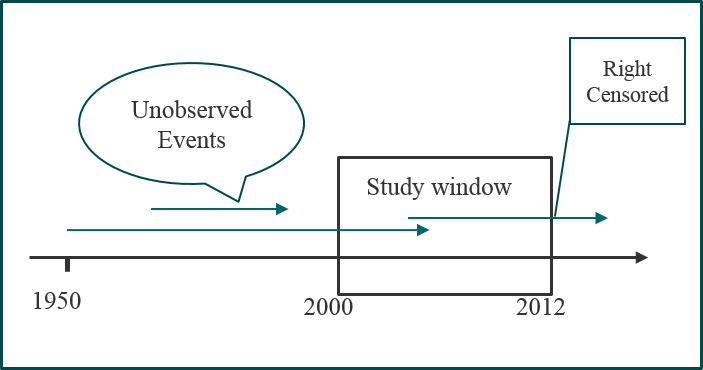
\includegraphics[width=3.5in]{fig1.png}
 	\caption{Right Censoring and Left Truncation}
 	\label{fig:1}
 \end{figure}
 Anyone that was an active employee during this period has their complete record included in the dataset whether or not their tenure began or ended outside of the study window.  Conversely, those employees whose tenure ended before the study window or for whom the start date occurred after the study window ended are not included in the study.

 Let $T$ be the time at which  an individual experiences the event of interest and let $C$ denote the final time at which the individual is observed. An observation is called {\it right censored} if $T> C$, indicating that actual event time for the individual is not recorded but is only known to be greater than $C$. Thus, employees that are currently active at the end of the observation window are right censored. These right censored observations do contain information, although incomplete, about a subjects lifetime and require special treatment in order to draw proper inference.
 \begin{align*}
 \delta_i&=
 \begin{cases}
 1   &\text{if  }  t_i \leq c_i \text{ (uncensored),}\\
 0   &\text{if  }  t_i > c_i \text{ (censored),}
 \end{cases}
 \end{align*}
 where, $i$ denotes the $i^{th}$ observation, and the failure time of event for $i^{th}$ observation is minimum time between $t_i$ and $c_i$, i.e., $min(t_i, c_i)$, that is when $c_i <t_i $, $c_i$ is taken as end time of the $i^{th}$ observation in order to do next  analysis.

 Left truncation is another interesting artifact of the window sampling scheme. Let $T$ again denote the time that the event of interest occurs and let $X$ denotes the time an individual enters the study. Only the individuals with $T \geq X$ are observed in the study window. Those individuals with $T \leq X$ are referred to as left truncated because they cannot be included in this study based on the sampling window as shown in the Figure \ref{fig:1}. Left truncation exaggerates the number of longer life individuals leading to a biased sample. To see this consider Figure \ref{fig:1}. The longest arrow represents a life span for an employee hired in 1950 and retiring in 2006. While this employee and any in his cohort that are still active are in the sample, others that began in 1950 but retired in 1998, for example, are not. Hence, because of the sampling window approach the longer someone continues working, the more likely they are to appear in our dataset.  We therefore see an overabundance of longer lived individuals in our data.  The presence of left truncation and the associated bias in the data must be taken into account to achieve accurate estimation of survival analysis \citep{carrion2010}.

 %Let $t_{i0}$ denotes the start time of the ith observation, i.e., hired time or age at %hired of ith employee, $x_{i}$ denotes the entry time of the ith observation, i.e., the %start time of study (November 1st, 2000) or age at November 1st, 2000. The start time of %the observation is maximum value between $t_{i0}$ and $x_i$, that is when $t_{i0} < x_i %$, $x_i$ is taken as start time of the ith observation in order to eliminate the left %truncation bias \citep{allison1995}. The number of failures in the $t_j$ is redefined for %left truncation. When $x_i < t_j \le t_i$, the observation is in the risk set. When %$t_{j} < x_i \le t_i$, the ith observation has not entered study yet at $t_j$ and it %cannot be considered in the risk set. When $x_i \le t_i < t_j$, it indicates the ith %observation whose failure time before $t_j$, and it cannot be considered in the risk set %at time $t_j$ neither \citep{carrion2010}.

% simulation study.

\subsection{Cox Proportional Hazards Regression Model} \label{Cox.mod}
%   1. what is cox ph regression model.
%   1. what is cox ph regression model.
The Cox proportional hazards (PH) regression model is the most widely used method for modelling lifetime data. The model was introduced in a seminal paper by \citet{cox1972}, one of the most cited papers in history. The Cox PH model is the canonical example of the semi-parametric family of models, specifying a parametric form for the effect of the covariates on an unspecified baseline hazard rate which is estimated non-parametrically.
The form of hazard model formula as shown in the equation \ref{eq:cox}:
\begin{equation}
	\label{eq:cox}
	h(t,x)=h_0(t)e^{(\sum_{i=1}^{k}\beta_ix_i)}
\end{equation}
where $x_i=(x_{i1}, x_{i2}, \ldots, x_{ik})$ are characteristics of individual $i$, $h_0(t)$ is the baseline hazard, and $\beta$  is a vector of regression coefficients.
%    why not parametric. baseline cannot fit to any parametric model\\
%    2. cox regression without/ with time dependent variable\\
%Stuff
The model provides an estimator of the hazard at time t for an individual with a given set of explanatory variables denoted by $x_i$.  In the standard Cox model, the linear combination $\sum_{i=1}^{k}\beta_i x_i$, is not a function of time $t$, and is called time-independent.  If $x_i(t)$ is a function of time the model is called the extended Cox model and is discussed in Section \ref{sec:coxt}. A key assumption for the model is the proportional hazards assumption. Proportional hazards assumes that explanatory factors have a strictly multiplicative impact on the hazard function so that different groups maintain a constant hazard ratio at all times. However, Cox regression can be extended to handle non proportional hazards using time-dependent variables or stratification; see \cite{kleinMosch2003}.

The Cox PH regression is "robust" and popular, because the baseline hazard function $h_0 (t)$ is an unspecified function and its estimation can closely approximate correct parametric model \citep{kleinbaum1998}. Taking the logarithm of both sides of the equation, the Cox PH model is rewritten in the equation \ref{eq:coxlog}:
\begin{equation}
	\label{eq:coxlog}
	\log{h(t,x)}=\alpha(t)+\sum_{i=1}^{k}\beta_ix_i
\end{equation}
where $\alpha(t)=\log{h_0(t)}$. If $\alpha(t)=\alpha$ i.e. constant, then the model reduces to the exponential distribution. As noted earlier, the general Cox PH model puts no restrictions on $\alpha(t)$.  The partial likelihood method is used to estimate the model parameters \citep{allison1995}. %The partial likelihood is estimated b baseline .
[NEED TO CHECK]

\subsection{Time Dependent Variable and Counting Process}
\label{sec:coxt}
Some explanatory variable values change over the course of the study. The extended Cox PH regression is a modification of the model that incorporates both unchanging time-independent variables as well as variables that change with time or time-dependent variables,
\begin{equation}
	\label{eq:timecovar}
	h(t,x)=h_0(t)e^{(\sum_{i=1}^{k_1}\beta_ix_i+\sum_{j=1}^{k_2}\gamma_jx_j(t))}
\end{equation}
where $x=(x_1, x_2, \ldots, x_{k_1}, x_1(t), x_2(t), \ldots, x_{k_2}(t))$, $h_0(t)$ is the baseline hazard occurring when $x=0$, $\beta$ and $\gamma$ are the coefficients of $x$. In order to fit this model, a modification of the partial likelihood is required and we often present the data set in a format called the {\it counting process} format in order to facilitate this calculation. The current study considers three internal time dependent variables that are functions of the individuals characteristics.
\begin{itemize}
\item Early Retirement Incentive Program (ERIP): a specific time during the study window, part of the 2008 calendar year, when the organization offered an early retirement incentive program; see \citep{ERIP}. It is time varying in the sense that it occurs at a different age for each individual in the study population and is set at 0 during the period when no program exists and 1 during the period when the program does exist.
\item Points 85 (P85): an indicator that an employee has amassed 85 service points, the sum of their years of service and age, and qualifies for full retirement benefits,
\item Age at 65 (A65): an indicator that an employee qualifies for retirement by exceeding the age 65 threshold
\end{itemize}
P85 and A65 are two additional time varying variables that capture important changes in individuals hazard level throughout the study.

%ERIP is a dummy variable across years:
%\begin{align*}
%ERIP&=
%\begin{cases}
%1   &\text{if employee works in year 2008,}\\
%0   &\text{if  employee does not work in year 2008.}
%\end{cases}
%\end{align*}

%What is counting process.   \\
The counting process format allows software packages to handle time dependent variables, by creating multiple intervals for each employee.  Each interval is defined so that the time varying variables are constant within the interval.
For example, for an individual that remained active until the end of the study and that achieved 85 points in December 2003, exceeded age 65 in December 2007, and received a retirement incentive in the 2008 calendar year, our study would include 5 records for the individual, November 2000 - November 2003, December 2003 - November 2007, December 2007, January 2008-December 2008, and January 2009 - December 2012, which is the end of the study.

Economic indicators represent another form of time dependent variables. These are referred to as external variables because they depend upon factors external to the employee. In models considering economic variables, monthly observations of economic indicators are aggregated at the yearly level leading to a larger number of time periods in the counting process format.  The economic variables are included at a one year lag since it is assumed that retirement and quitting decisions are made a significant time in advance of the actual event and therefore depend on older values of these indicators.  Importantly, using lagged quantities allows the model to be used for forecasting for a 12 month period since these numbers will be known at the time of forecast.

The start and end points of each interval are given in the definitions below.
\begin{equation}
	\label{eq:interval}
	\begin{split}
		(\text{start point}, \text{end point})= (max(\text{hired date}, \text{January 1 of a certain year}),\\
		min(\text{terminated date}, \text{December 31 of a certain year}))
	\end{split}
\end{equation}



\subsection{Stratification and Multiple Baselines}
%I. what is stratification model;\\
An alternative for handling nonproportional hazards is stratification.  A stratified model allows each subgroup of data as defined by a grouping variable to have its own baseline hazard while sharing parameters for other variables across. If the proportional hazards assumption holds within these subgroups then this model allows us to get valid common estimates of variable effects using all of the observations. Equation \ref{eq:strata} below represents the hazard function for strata {\it z};
\begin{equation}
	\label{eq:strata}
	h(t,x,z)=h^z_0(t)e^{(\sum_{i=1}^{k}\beta_ix_i)}
\end{equation}
where $z$ represents the grouping variable, and $h^z\sigma_0(t)$ is a baseline hazard based for stratam z and $\beta_i$ are common effects of variables. Note that the strata variables cannot be the variables in the Cox PH model.

%II. how to select a stratify variable\\
%The proportional hazard assumption can be tested using Schoenfeld residuals which works even if the model includes time-dependent variables; see \citet{allison2010,collett2015}. An alternative is to test the interaction between time-dependent and time-independent variables in the Cox PH model. The assumption is valid if the interaction is not statistically significant ($P>0.05$).  Including a stratified variable, when appropriate, can improve the Cox model's performance.  The C-statistic is used to compare models with and without stratification with a higher C value indicating a better model \citep{lemke2012}.
%I. what is stratification model;\\
%When the proportional hazards assumption fails there are several alternative approaches to capturing observed hazard patterns. One approach for handling nonproportional hazards is stratification.  A stratified model contains a separate baseline hazard for each subgroup defined by the analyst while allowing shared effects of other factors. If the proportional hazards assumption holds within these subgroups then this model allows us to get valid common estimates of variable effects using all of the observations. Equation \ref{eq:strata} below represents the hazard function for strata {\it z};
%\begin{equation}
%\label{eq:strata}
%h(t,x,z)=h^z_0(t)e^{(\sum_{i=1}^{k}\beta_ix_i)}
%\end{equation}
%where $z$ represents one level of the grouping variable $Z$, $h^z\sigma_0(t)$ is a baseline hazard for this individual subgroup and $\beta_i$ are constant effects of variables across all strata. Note that a variable cannot be used as both a stratification variable and a constant effect in the Cox PH model.

%II. how to select a stratify variable\\
\subsection{Testing the PH Assumption}
Three common approaches areavailable for testing the validity of the proportional hazard assumption: The first approach is to investigate the Schoenfeld residuals. A second alternative is to test the interaction between time-dependent and time-independent variables in the Cox PH model. The PH assumption is valid if the interaction is not statistically significant ($P>0.05$). Finally, including separate baseline hazards for each strata defined by the analyst can also capture variation in changes of the hazard rate. See \citet{allison2010,collett2015} for more details on these tests.

%Including a stratified variable, when appropriate, can improve the Cox model's %performance.  The C-statistic is used to compare models with and without %stratification with a higher C value indicating a better model \citep{lemke2012}.

\subsection{Competing Risks}
%  what is competing risks. competing ricks can help forecasting employee retirement and voluntary quit. \\
%  why select these two reasons to model.\\
One of the many nuances observed within this data set is the fact that currently employees can leave employment in several mutually exclusive ways.  These include leaving due to quitting voluntarily, being laid off, dismissed for cause, transferred, retired, or being unable to continue due to disability or death. A competing risk is an event whose occurrence either precludes the occurrence of the event of interest or fundamentally alters the probability of occurrence of this event of interest \citep{tableman2003}.  A competing risks model is a common approach when studying a single mode of leaving such as retirement if subjects at risk may also exit through an alternative mode such as quitting.  In the current study, when considering retirement as the event of interest and voluntary quitting as a competing risk, all observations are initially included in the study and outcomes that end in a quitting event are treated as censored which allows their observed work period to be used informatively.
% \ref{eq:competing}:
%  \begin{equation}
%  \label{eq:competing}
%  h_j(t,x)=h_{j0}(t)e^{(\sum_{i=1}^{k}\beta_{ij}x_i)}
% \end{equation}
%  where, $x_{j}$ is the variable for a specific type of turnover. Note that the %coefficient $\beta$ is the effects of the variables may be different from different %turnover types. If $\beta_{ij}$  is the same for all j, the model simplified to Cox %PH model as shown in equation \ref{eq:cox}.


\subsection{Variable Selection and Model Choice} \label{sec:modelchoice}
In the current study two equivalent time measurements were considered as response variables for modelling, AGE in years and YCS.  Because of the inclusion of time varying explanatory variables, and the need to estimate the baseline hazard for purposes of forecasting, the data must be formulated as a counting process , see Section \ref{sec:coxt}.  After some consideration, age was considered the better option for analysis because the more condensed distribution of values allows more accurate estimates of the baseline.

The model selection initiated by considering DIV, AGC, GENDER and other time independent variables as well as ERIP, P85, and A65. We removed non-significant variables using the criteria that p-values should be less than $.05$ and starting with the largest p-value first, i.e. backwards selection.  This continued until only statistically significant variables remained.  We also tested stratifying the baseline using occupational code, which did not improve the model. Finally we tested external time varying covariates, which capture economic factors, one at a time and noted the impact on model performance.

%All the variables were then included in the Cox PH regression model and selected by %manually backwards selection method based on $P<0.05$.  The variable selection procedure is as follow: first, all the variables are used to build the model. Second, remove the non-significant variable ($P>0.05$) with the largest P value, and rerun the model with the other variables. Then, repeat the second step until there is no significant variable remaining in the model.

\subsection{Model Evaluation and Comparison}
%\subsubsection{Measurements}
%AIC, BIC, MAPE, c statistic.\\

In order to evaluate the models considered in this study, the data were first split into two sets, a training set containing all of the observations from years 2000-2010 and a testing set containing events on the same individuals that occurred in calendar years 2011 and 2012. The testing (holdout) sample was included to get an accurate measure of how well the model would forecast beyond the observed data.  Because the testing data set is not included in the model fitting process, this out of sample evaluation provides a better estimate of predictive accuracy, see \citet{kuhn2013} for further discussion of this approach.

All of the fitted models considered in this study are first evaluated by four statistical criteria:  Akaike’s Information Criterion (AIC), Schwartz’s Bayesian Criterion (SBC), mean absolute percentage error (MAPE) and likelihood based goodness of fit $G^2$. Ideally, the optimal model should minimize the values of AIC, SBC, MAPE, and $G^2$ when fit to the training data. In this study, the model performance on holdout dataset is considered more important than that on the training dataset.
AIC and SBC both assess model fit by balancing a larger likelihood value with a penalty that increases with the number of variables included.  The inclusion of the penalty term diminishes the potential for over-fitting \citep{allison2010,hosmer2013}. These measures are generated automatically by the model fitting process.

%C-statistics or the area under the receiver operating characteristic (ROC) curve is to test whether the probability of predicting the outcome is better than chance. It ranges from 0.5 to 1.  Models are considered acceptable when the C-statistic is higher than 0.7 \citep{hosmer2013}. C-statistics are calculated by using the predicted failure probability compared with the actual outcomes by SAS proc logistic.
In order to asses predictive measures such as MAPE and $G^2$ we first predict the probability of the event of interest, e.g. retirement, for each active individual during each calendar year of the training or testing data set.  For each employee, we compute the conditional probability of the event occurring between time $t_j$ and $t_{j-1}$, given that the employee is active at time $t_{j-1}$. It is calculated using the baseline hazard and coefficients from Cox PH models as shown in Equation \ref{eq:prob} below
\begin{equation}
\label{eq:prob}
\begin{split}% to allgin the equation
P\{t_{j-1}<T<t_j|T \ge t_{j-1}\} &=1-P\{T>t_j|T \ge t_{j-1}\}\\
&=1-\frac{S_k(t_j)}{S_k{(t_{j-1})}}   \\
&=1-\frac{{S_0(t_j)}^{(\sum_{i=1}^{p}\beta_ix_i)}}{   {S_0(t_{j-1})}^{(\sum_{i=1}^{p}\beta_ix_i)}}
\end{split}
\end{equation}
where, $T_k$ is survival time of the $k^{th}$ individual , $t_j$ is a specific time value, $S_k(t) = {S_0(t_j)}^{(\sum_{i=1}^{p}\beta_ix_i)}$ is the survival function for the $k^{th}$ individual, $S_0(t)$ is the baseline function generated by Cox PH model, $x_i$ are the individual explanatory variables, and $\beta_i$ are the respective regression coefficients for the variables.

MAPE is common measure for computing the accuracy of predictions from a forecast model and is often used to compare models since it measures relative performance \citep{chu1998}. MAPE is calculated as the average percent deviation of a forecast from the actual observation,
\begin{equation}
\label{eq:mape}
MAPE=\sum_{t=1}^{n}\left | \frac{y_t-\hat{y_t}}{y_t} \right |\frac{1}{n}\%
\end{equation}
Our implementation of MAPE for retirement predictions used the yearly actual and predicted numbers of retirements number as $y_t$ and $\hat{y_t}$. The predicted yearly retirement number, $\hat{y_t}$,  is the expected retirement count for a particular year and is computed as the sum of conditional probabilities given by Equation \ref{eq:prob} over currently active employees.  This follows from the fact that the probability of each employee retiring can be viewed as an independent Bernoulli random variable.

%\begin{equation}
%\label{eq:expturnover}
%E(\text{turnover number at } t_j)=\sum_{i=1}^k{P_i\{t_{j-1}<T<t_j\}}
%\end{equation}
%where, $i$ denotes the ith employee.

Although less common in forecasting, $G^2$ is another useful criteria for evaluating model prediction for dichotomous events \citep{Simonoff2013}. The calculation takes the form,
\begin{equation}
\label{eq:g2}
G^2=2\sum_{t}[y_t\log{(\frac{\bar{p_t}}{\hat{p_t}}})+ (n_t-y_t)\log{(\frac{1-\bar{p_t}}{1-\hat{p_t}}})]
\end{equation}
where, $y_t$ is the number of employees retired in year $t$, $n_t$ is the workforce number in year $t$, $\bar{p_t}={y_t}/{n_t}$ is the observed proportion of events, and $\hat{p_t}={\hat{y_t}}/{n_t} $ is the model predicted number of events.  Small values of $G^2$ indicate close agreement of observed and predicted numbers of events.

%%%%%%% need some explain for traing and holdout mape%%%%%%%%%%%
%The logistic regression and time series moving average methods are also employed to compare with the  performance of Cox PH regression model by MAPE value and $G^2$.
%The evaluation step is to calculate the yearly predicted turnover number for training and holdout dataset, and then compared the predicted number with the actual number.


%add evaluation formula.

%\subsubsection{Model validation}
% 1. Forecast employee turnover   how to forecast and calculate employee turnover number\\
% 2. conditional probability (The prediction is conditional probability): given the employee is survival at last year, what is the probability they survival or quit for this year.\\
% 3. the total number of employee turnover is the aggregate all turnover probabilities of employees at each year\\
%
% 4. split data into two ways: both training and holdout, training to build the model and holdout is to validate the model, and compare the actual vs forecasting, calculated MAPE and C statistics. \\
%       WAY1: training (10 years)and holdout (2 years). forecasting the total number of employee leaving the organization, compared to the actual number to calculate MAPE and C statistics. compare to logistic regression and time series methods to shown survival is better.\\
%       WAY2: random split the data into training (2/3) and holdout (1/3), using c statistics to select one best survival model.
 \section{Simulation Studies of Proportional Hazards Models}

The goal of the proposed data analysis is to create a predictive model for retirement and other types of turnover based on a database of employees.  Section \ref{bias}, pointed out two sources of bias present in the data, left truncation and right censoring.  Because the Cox PH model is estimated using a partial likelihood that depends only upon the cases at risk at the specific failure times, estimates of regression coefficients should remain unbiased and efficient in the presence of left truncation and right censoring \citep{Harrell2002}.  What is less clear is the impact of the bias on model predictions. This stems from the fact that model predictions depend upon both the baseline, estimated using non-parametric methods, and the parametric estimates of the regression coefficients.  In addition, a third ever-present challenge, model selection, may also impact predictions to a significant degree.

In order to better understand the effect of various levels of truncation and censoring on the predictions we perform 3 simulation studies based on Weibull simulated data with varying amounts of bias.

The basic setup in all three simulations is the same. Data sets of sizes $n =100, 200, 500,$ $1000, 2000,$ $\text{and } 4000$ were generated from a Weibull regression model which was a function of 1 explanatory variable, which we refer to as $age$.  In the simulation, $age$ is uniformly distributed from 22 to 70 years, a range that is chosen to mimic the actual distribution of worker ages observed in our sample.

The baseline hazard for Weibull distribution with shape $\alpha$ and scale $\lambda$ is $h_0(t)=\alpha(\lambda)^\alpha t^{\alpha-1}$.  Extending this to a hazard from a proportional hazards regression model for $age$, we simply multiply by the exponentiated linear predictor shifting the baseline up or down,
\begin{equation} \label{eq:weibull}
\begin{split}% to allgin the equation
h(t|age) & =h_0(t)exp(\beta \times age) \\
&=\alpha (\lambda (exp(\beta \times age)^{\frac{1}{\alpha}})^\alpha t^{\alpha-1} \\
&=\alpha(\tilde{\lambda} )^\alpha t^{\alpha-1}
\end{split}
\end{equation}
where, $\tilde{\lambda}=\lambda (exp(\beta \times age)^{\frac{1}{\alpha}}$.

The survival times $T_i$ are randomly generated from the Weibull distribution with shape parameter $\alpha=1.5$ and $\tilde{\lambda}=exp(1.5 +0.025 \times age)^{\frac{1}{\alpha}}$.  It follows that $\lambda = e^1$.

%
%\subsection{TEMP MODEL}
%%In order to understand the performance and efficiency of the Cox PH model in right censored and left truncated data we perform a simulation study.
%
%%Generated $n =100, 200, 500, 1000, 2000, \text{and } 4000$ observations  from a Weibull regression model  with one variable which we referred to as age.
%
%%Age is uniformly distributed from 22 to 70 years of age, which is chosen to mimic the actual distribution of workers ages in our sample.
%
%%In the regression model, the coefficients for $\beta_{age} = -.025$ (Why?) and the coefficient for $\beta_0 = 1.5$.
%
%The survival times $T_i$ are randomly generated from a Weibull distribution with shape parameter $\alpha$ and scale parameter $\lambda$, where $\alpha=1.5$ and $\lambda=exp(-0.025age+\beta_0)^{\frac{1}{\alpha}}$.
%
%The simulation is used to examine Cox PH model predictive performance with right censor and left truncation. The simulated lifetime data is generated based on the Weibull distribution. The hazard function for Weibull regression model with shape parameter $\alpha$, scale parameter $\lambda$, and variable $X$ is shown in equation \ref{eq:weibul}, given $h_0=\alpha(\lambda)^\alpha t^{\alpha-1}$:
% \begin{equation} \label{eq:weibul}
% \begin{split}% to allgin the equation
% h(t|X) & =h_0(t)exp(\beta X) \\
%          &=\alpha (\lambda (exp(\beta X)^{\frac{1}{\alpha}})^\alpha t^{\alpha-1} \\
%          &=\alpha(\tilde{\lambda} )^\alpha t^{\alpha-1}
% \end{split}
% \end{equation}
% where, $\tilde{\lambda}=\lambda (exp(\beta X)^{\frac{1}{\alpha}}$.
%The simulation can be described as follows. The sample size was n=100, 300, 500, 1000, and 4000, with one variable $X$, named Age, which follows uniform distribution with parameter $a$ $(a=22)$ and $b$ $(b=70)$. Only one variable age is used in simulation process to make the estimation procedure simple and close to real world. The coefficient $\beta_{age}$ is taken $-0.025$ and $\beta_0=1.5$.
%Then, the survival time $T$ is random generated for each observation based on Weibull distribution with shape parameter $\alpha$ and scale parameter $\lambda$, where $\alpha=1.5$ and $\lambda=exp(-0.025age+\beta_0)^{\frac{1}{\alpha}}$.
%The simulation is performed on right censoring and left truncation separately, in order to observe the effects for different bias.
%

The simulations are performed using the {\tt coxreg} and {\tt phreg} functions from the {\tt R}-package {\tt eha} \citep{eha} for model fitting.  Function {\tt coxreg} performs a standard Cox PH regression using the partial likelihood to fit the model.  The {\tt phreg} function performs a parametric proportional hazards regression using both Weibull, Extreme value (EV) baselines.

%Total predicted failure number is calculated as shown in equation \ref{eq:prob} and \ref {eq:expturnover}. The actual and predicted failure number are compared to show right censor and left truncation's impacts on the coefficient and baseline estimation .
%For right censor and left truncation simulation, the Cox regression models are modeled by "coxreg" and "phreg" function in eha package.


\subsection{Simulation 1: Right Censoring} \label{rightcensor.sim1}

The first study focuses on understanding the impact of right censoring, a significant effect in the turnover data analyzed later due to the many employees that remain active for the entire observation window. For each of the sample sizes above, survival times $T_i$ are simulated from the Weibull distribution as described earlier.  Four censoring times $C_j$ are defined as the first, second, third, and fourth(maximum) quartiles of the simulated sample of lifetimes and refer to 75\%, 50\%, 25\% and 0\% censoring proportions respectively. If the survival time $T_i$ of the $i^{th}$ observation is below the censoring time ($C_i$), then the lifetime $T_i$ is observed and the censoring indicator $\delta_i=1$. When the survival time $T_i$ for $i^{th}$ observation is greater than the censoring time ($C_i$), then the censoring time $C_i$ is observed and censoring indicator $\delta_i = 0$.

The results of 100 simulations at each combination of sample size and censoring proportion are shown on the left side of Table \ref{tab:rightcensor}. Column 1 gives the censoring proportion, column 2 the observed number of events before censoring, and columns 3 and 4 are the average $\beta_{age}$ estimates over 100 simulations for both {\tt coxreg} and {\tt phreg}.  The values in columns 5 \& 6  are the average estimates of $\lambda$ and $\alpha$ from the parametric fit of {\tt phreg}. The simulation results show censoring proportion and the number of events are two influential factors for the coefficient estimation. The model overestimates the coefficients of age, $\lambda, \text{ and } \alpha$, when the dataset has a high proportion of censoring. For example, when 75\% of the data are censored with only 25 events, the estimates for three parameters are 0.028, 4.043, and 1.564, respectively, which are the highest among all the estimates. As the event number increases, the estimates approach the actual value. For example, the estimation of age, $\lambda, \text{ and } \alpha$ are close to 0.025, 2.7, and 1.5, respectively, as the number of events exceeds 500.

%[Discuss Predictions]The predicted number of events are shown [What does this say about censoring effect on predictions?] in the sixth column is the total predicted failure number calculated by applying the coefficient estimates and the non-parametric baseline from Cox PH models into the dataset without considering censoring. The predicted events using censoring models are all lower than the actual total failure number, but close to the number of events after censoring.

 %[NOTE: Important point is that baseline hazard and predictions vary slightly with uncertainty, ??] The baseline does not include hazards or survival probability information for the long life time observation, because the baseline just captures the events before the censor time and the observation with long life time are censored in this simulation. As a result, there is no failure probability for long life time observation.

 \begin{table}[!htbp]
 	\renewcommand{\arraystretch}{1.5}
 	\scriptsize %table fond
 	\centering
 	\caption{Right Censoring and Left Truncation Simulation Statistics}
 	\begin{tabular}{@{}C{1.8cm}lllll||C{1.8cm}lllll@{}}
 		\toprule
 		\multicolumn{6}{c}{Right Censor}  & \multicolumn{6}{c}{Left Truncation}                \\ \midrule
 		Right Censor Proportion & Events & $\beta_{coxreg}$ & $\beta_{phreg}$ & $\lambda_{ph}$
 		& $\alpha_{ph}$ & Left Truncation Proportion & Events &$\beta_{coxreg}$ & $\beta_{phreg}$ & $\lambda_{ph}$ & $\alpha_{ph}$ \\
 		\midrule
 		0\% & 100    & 0.026   & 0.027 & 2.931 & 1.509 & 0\%   & 100  & 0.027 & 0.027 & 2.865 & 1.534 \\
 		25\% & 100    & 0.027  & 0.027 & 2.962 & 1.527 & 25\%  & 75   & 0.027 & 0.027 & 2.917 & 1.546 \\
 		50\% & 100    & 0.028  & 0.028 & 3.237 & 1.530 & 50\%  & 50   & 0.027 & 0.027 & 2.899 & 1.577 \\
 		75\% & 100    & 0.028  & 0.028 & 4.043 & 1.564 & 75\%  & 25   & 0.029 & 0.029 & 3.280 & 1.757 \\
 		0\%  & 200    & 0.026  & 0.026 & 2.841 & 1.508 & 0\%   & 200  & 0.025 & 0.025 & 2.777 & 1.506 \\
 		25\% & 200    & 0.026  & 0.026 & 2.856 & 1.513 & 25\%  & 150  & 0.025 & 0.025 & 2.756 & 1.515 \\
 		50\% & 200    & 0.026  & 0.026 & 2.925 & 1.527 & 50\%  & 100  & 0.025 & 0.025 & 2.825 & 1.532 \\
 		75\% & 200    & 0.026  & 0.026 & 3.167 & 1.540 & 75\%  & 50   & 0.026 & 0.026 & 2.927 & 1.572 \\
 		0\%  & 500    & 0.025  & 0.025 & 2.731 & 1.500 & 0\%   & 500  & 0.025 & 0.025 & 2.732 & 1.509 \\
 		25\% & 500    & 0.025  & 0.025 & 2.718 & 1.508 & 25\%  & 375  & 0.025 & 0.025 & 2.737 & 1.514 \\
 		50\% & 500    & 0.025  & 0.025 & 2.744 & 1.514 & 50\%  & 250  & 0.026 & 0.026 & 2.778 & 1.514 \\
 		75\% & 500    & 0.025  & 0.025 & 2.787 & 1.525 & 75\%  & 125  & 0.026 & 0.026 & 2.835 & 1.547 \\
 		0\%  & 1000   & 0.025  & 0.025 & 2.748 & 1.509 & 0\%   & 1000 & 0.025 & 0.025 & 2.710 & 1.504 \\
 		25\% & 1000   & 0.025  & 0.025 & 2.747 & 1.512 & 25\%  & 750  & 0.025 & 0.025 & 2.709 & 1.504 \\
 		50\% & 1000   & 0.025  & 0.025 & 2.748 & 1.514 & 50\%  & 500  & 0.025 & 0.025 & 2.715 & 1.506 \\
 		75\% & 1000   & 0.026  & 0.026 & 2.844 & 1.509 & 75\%  & 250  & 0.025 & 0.025 & 2.694 & 1.524 \\
 		0\%  & 2000   & 0.025  & 0.025 & 2.714 & 1.502 & 0\%   & 2000 & 0.025 & 0.025 & 2.740 & 1.503 \\
 		25\% & 2000   & 0.025  & 0.025 & 2.713 & 1.503 & 25\%  & 1500 & 0.025 & 0.025 & 2.731 & 1.502 \\
 		50\% & 2000   & 0.025  & 0.025 & 2.742 & 1.500 & 50\%  & 1000 & 0.025 & 0.025 & 2.724 & 1.503 \\
 		75\% & 2000   & 0.025  & 0.025 & 2.733 & 1.502 & 75\%  & 500  & 0.025 & 0.025 & 2.718 & 1.508 \\
 		0\%  & 4000   & 0.025  & 0.025 & 2.719 & 1.504 & 0\%   & 3999 & 0.025 & 0.025 & 2.720 & 1.500 \\
 		25\% & 4000   & 0.025  & 0.025 & 2.718 & 1.505 & 25\%  & 3000 & 0.025 & 0.025 & 2.722 & 1.501 \\
 		50\% & 4000   & 0.025  & 0.025 & 2.724 & 1.503 & 50\%  & 2000 & 0.025 & 0.025 & 2.710 & 1.502 \\
 		75\% & 4000  & 0.025 & 0.025  & 2.729 & 1.513 & 75\%  & 1000  & 0.025  & 0.025 & 2.703 & 1.503 \\ \bottomrule
 	\end{tabular}
 	\label{tab:rightcensor}%
 \end{table}



\subsection{Simulation 2: Right Censoring with Staggared Entry Times} \label{rightcensor:sim2}

In order to more accurately capture the nuances and complexities of the data sampling scheme and understand the impact of right censoring we modify the above simulation by staggering the entry times.  Starting with the Weibull simulated failure times, we add offset factor $S$ that follows a uniform distribution from 0 to 10 and represents variation in the starting times of the employees within the study window. The event time is equal to the summation of start point and survival time: $S+T$. The censoring time is a single fixed value that ensures a fixed proportion (25\%, 50\%, and 75\%) of censored observations.  The observation and censoring indicator are then determined as in the first simulation with the survival time for an individual being $min(C,T_i+S_i) - S_i$. Because some observations start after the cutoff point (censor time) the sample sizes would vary for different censoring proportions.  To ensure constant sample size, 6000 observations are initially simulated and 400 whose start point occur before the censoring point are randomly selected.
 \begin{table}[htbp]
 	\renewcommand{\arraystretch}{1.5}
 	\scriptsize %table fond
 	\centering
 	\caption{Right Censor Simulation Results by Various Start Time}
 	\begin{tabular}{ccccccc}
 		\toprule
 		\multicolumn{1}{c}{\multirow{2}{1.5cm}{Censoring Pct.}}  & \multirow{2}[4]{*}{Events} & \multicolumn{3}{c}{Variable Estimates} & \multicolumn{2}{c}{Predicted Events} \\ \cline{3-7}
 		&       & $age$   & $\lambda$ & $\alpha$ & "coxreg" & "phreg" \\
 		\midrule
 		0\%   & 400   & 0.025 & 2.694 & 1.508 & 398.52 & 400.44 \\
 		25\%  & 400   & 0.026 & 2.802 & 1.518 & 394.24 & 401.72 \\
 		50\%  & 400   & 0.026 & 2.828 & 1.514 & 340.73 & 398.51 \\
 		75\%  & 400   & 0.025 & 2.821 & 1.518 & 215.92 & 400.80 \\
 		\bottomrule
 	\end{tabular}%
 	\label{tab:right2}%
 \end{table}%

The results of the simulation are shown in Table \ref{tab:right2}. As discussed above, both a correctly parametric proportional hazards regression model with a Weibull baseline {\tt phreg} and a semi-parametric Cox regression {\tt coxreg} are fit in order to evaluate differences in efficiency. The estimation of age and $\alpha$ are all close to the true values (0.025 and 1.5) when averaged over 100 simulations.  Based on 400 events, the estimates of $\lambda$ increase from 2.694 with no censoring to over 2.8 when censoring is above 50\%.  In general, the results indicate that right censoring has little impact on coefficient estimation and that the semi-parametric estimates show similar efficiency to fully parametric estimates. However, right censoring does impact estimation of the  baseline function for the Cox PH model as shown in the 6th and 7th columns of the Table and Figure \ref{fig:rightbase}.  Panel (a) shows no censoring and the parametric baseline matches the non-parametric although as time increases and the number at risk decreases we see that non-parametric estimate deviates more strongly from the parametric fit.  Panel (b) shows 25\% censoring for 100 replications.  We see that, as the range of the data decreases, the duration of the non-parametric baseline estimate is more restricted, while the parametric fit can be extrapolated with the usual caveats.  In panel (d), the 75\% censoring level, we see increased variability even with the diminished range due to the more restrictive censoring time.  Note that these results are indicative of monotonically increasing hazards and may differ if we consider other baseline distributions

\begin{figure}[h!]
	\centering
	\subfloat[0\% Right Censoring ]{\label{fig:baseno}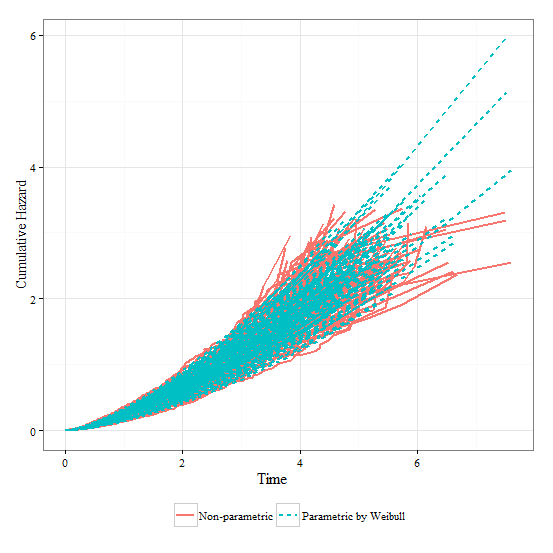
\includegraphics[width=3in]{base0.png}}
	\quad
	\subfloat[25\% Right Censoring]{\label{fig:base25}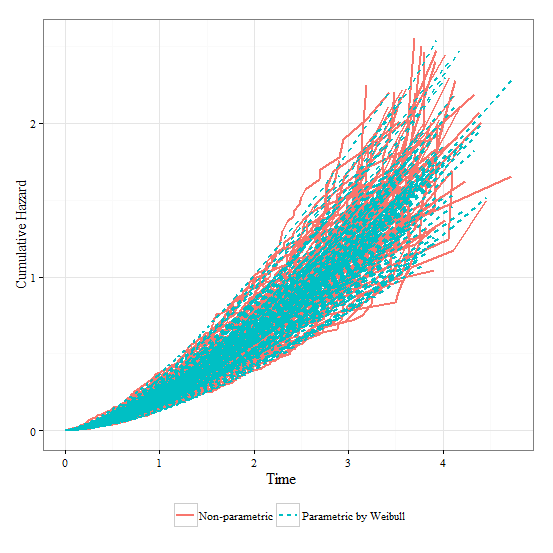
\includegraphics[width=3in]{base25.png}}
	\quad
	\subfloat[50\% Right Censoring ]{\label{fig:base50}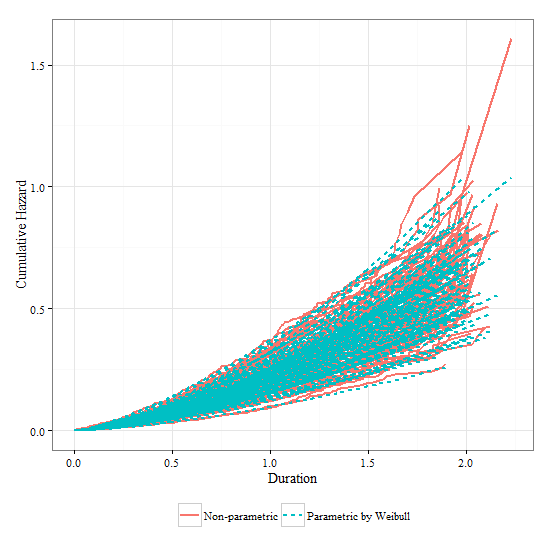
\includegraphics[width=3in]{base50.png}}
	\quad
	\subfloat[75\% Right Censoring]{\label{fig:base75}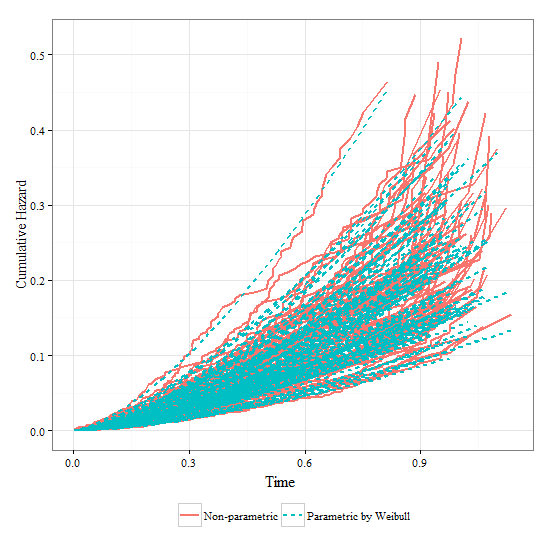
\includegraphics[width=3in]{base75.png}}
	\caption{Baseline Comparison by Various Censoring}
	\label{fig:rightbase}
\end{figure}


[PARAMETRIC BOOTSTRAP DISTRIBUTION-LOOK AT RESEARCH, ALSO SIMONOFF PAPER]

Figure \ref{fig:rightdiff}, panels (a-d) illustrate the difference between parametric and non-parametric estimates of the baseline cumulative hazard function, $H_0(t) = -log(\hat{S}(t))$ at different time points over 100 simulated data sets.  Panel (a) indicates that without censoring, overall survival estimates including both baseline and covariates are very similar across parametric and semi-parametric approaches.  As lifetime, $t$ increases, we see increasing deviations between the two estimates.  This due both to the cumulative nature of the estimates and to the increasing variability of hazard estimation of the non-parametric baseline, the Breslow estimator,   \citep{DavHink1997,Burr1994} as the number of observations at risk diminishes over time.

\begin{figure}[h!]
	\centering
	\subfloat[No Right Censoring]{\label{fig:diffno}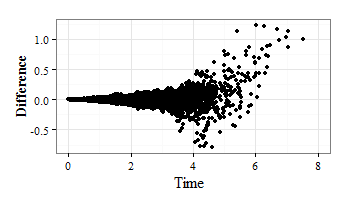
\includegraphics[width=3in]{diff0.png}}
	\quad
	\subfloat[25\% Right Censoring]{\label{fig:diff25}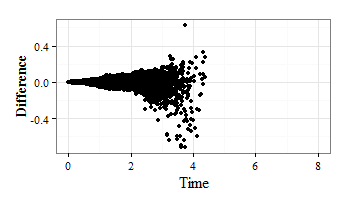
\includegraphics[width=3in]{diff25.png}}
	\quad
	\subfloat[50\% Right Censored ]{\label{fig:diff50}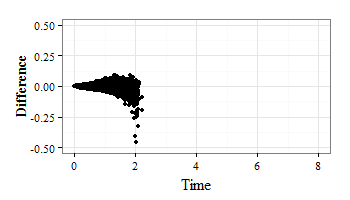
\includegraphics[width=3in]{diff50.png}}
	\quad
	\subfloat[75\% Right Censoring]{\label{fig:diff75}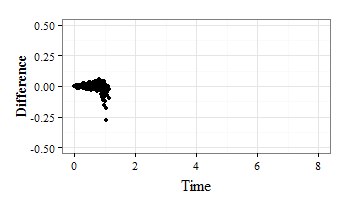
\includegraphics[width=3in]{diff75.png}}
	\caption{Differences in Estimates of Baseline Cumulative Hazard Functions, Parametric - Non-parametric, for 4 Levels of Censoring}
	\label{fig:rightdiff}
\end{figure}
When censoring is introduced in panel (b) we see that the range of the x axis is restricted.  Although this varies slightly across simulations, it is clear that the non-parametric estimator cannot estimate survival probabilities beyond the maximum observed lifetime due to the lack of a parametric model for the baseline.  In the current simulation, this was dictated by the censoring time, which was set to ensure a fixed proportion of censored cases.  In real studies, such as the one introduced in Section \ref{application}, the maximum observed lifetime will be dictated by the population and the sampling window.  Panels (c) and (d) reiterate both of these factors. As the censoring level increases to 50\% and finally 75\%, the range of non parametric baseline estimate is further restricted but the accuracy improves due to the increasing concentration of observations before the censoring time.  Because all simulations had 400 observations, 75\% censoring ensures 100 events before the censoring point, which is close to 1 providing a very accurate estimate of the baseline and less dispersion than the uncensored data.  Parametric models do not suffer from limitations on the baseline estimate, a seeing advantage, but instead require careful model selection steps which introduce other challenges.
 % Table generated by Excel2LaTeX from sheet 'Sheet2'


\subsection{Left Truncation Simulation}

Finally, we perform a simulation to evaluate the impact of left truncation bias on parameter estimation and prediction. Again, we begin by generating a simulated sample of employment times $T_1, \ldots, T_n$.  For each observation, $i$, a uniform random variable $S_i \sim U(0,max(T))$ is then generated and represents the simulated employee starting time. The event time is then $R_i = S_i+T_i$. Figure \ref{fig:trunchist} provides a histogram of the simulated population of $R_i$. Four levels of truncation are introduced by shifting the beginning of the sampling window, $L$ from 0 across the quartiles of $R$ . When the starting for $ith$ observation, $S_i$, is less than truncation time $l_i$, the observation starting point is reset to $l_i$ which is the first point that the employee is observed in the sampling window. If $S_i> l_i$, then the employee is first observed at $S_i$, which remains the starting point.  If $R_i>C$, where $C$ represents the end of the observation window, then the employee is still active at the end of the sampling window and their turnover time is censored.  In order to isolate the impact of truncation bias, no censored values were generated in this study.

\begin{figure}[h!]
	\centering
    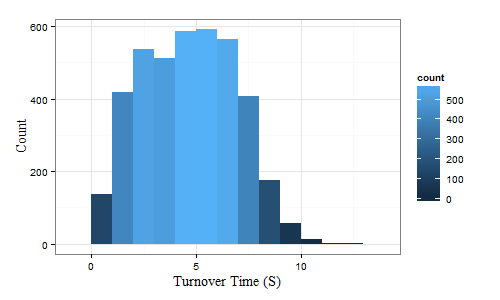
\includegraphics[width=3.5in]{truncationhist.png}
	\caption{Histogram of Simulated Lifetimes}
 	\label{fig:trunchist}
 \end{figure}

Sample size and censoring proportions and results follow the same protocol given in Section \ref{rightcensor.sim1}.  The results of the simulation are shown on the right side of Table \ref{tab:rightcensor}.  As before, values shown represent average parameter estimates over 100 replications for the Cox model and a Weibull PH.  The general pattern suggests that as truncation proportion increases for a fixed number of events, the parameter estimates become slightly biased.  In the Cox PH case when the sample size is 100, the coefficient for age increases from .027 to .029 as the truncation increases from 0\% to 75\%.  The scale parameter for the parametric model, {\tt phreg}, also increases with truncation percentage.  For samples of size 100, with $\lambda = e^1 \approx 2.718$ the average estimate increases from $2.865$ with no truncation to $3.280$ with 75\% truncation.  Estimates for $\alpha = 1.5$ increase from 1.534 to 1.757. Such effects disappear as the number of events increase.
 \begin{figure}[h!]
 	\centering
 	\subfloat[No Left Truncation]{\label{fig:ev0}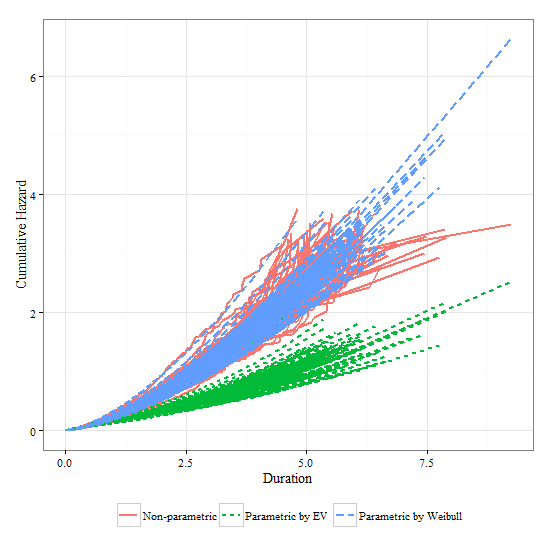
\includegraphics[width=3in]{EV0.png}}
 	\quad
 	\subfloat[25\% Left Truncation]{\label{fig:ev25}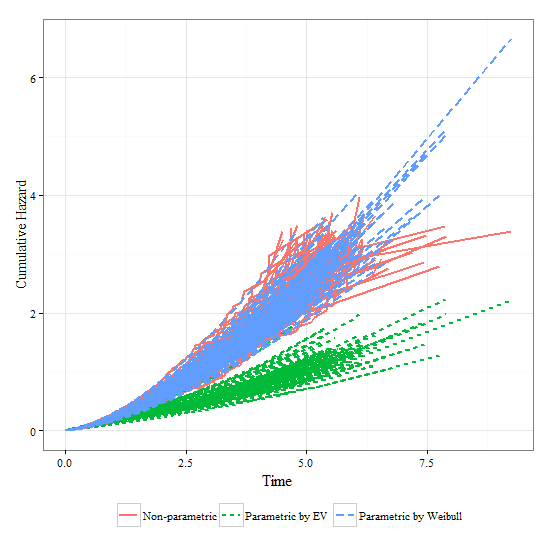
\includegraphics[width=3in]{EV25.png}}
 	\quad
 	\subfloat[50\% Left Truncation]{\label{fig:ev50}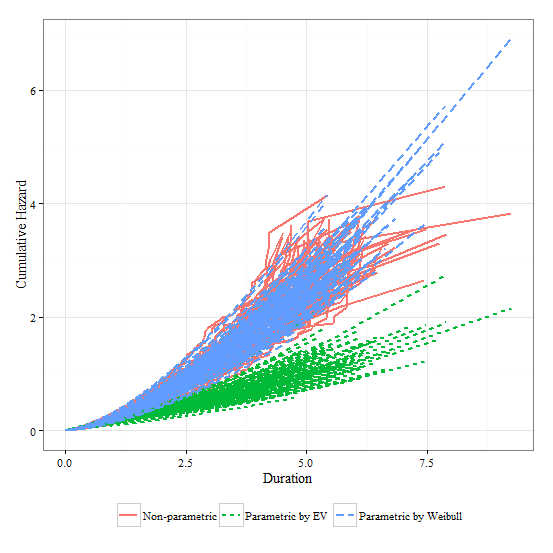
\includegraphics[width=3in]{EV50.png}}
 	\quad
 	\subfloat[75\% Left Truncation]{\label{fig:ev75}\includegraphics[width=3in]{EV75.png}}
 	\caption{Left Truncation Simulation Predictions: Comparison of Actual vs. Cox PH and Parametric PH with EV baseline.}
 	\label{fig:leftbase}
 \end{figure}

 \begin{figure}[h!]
 	\centering
 	\subfloat[No Left Truncation]{\label{fig:leftno}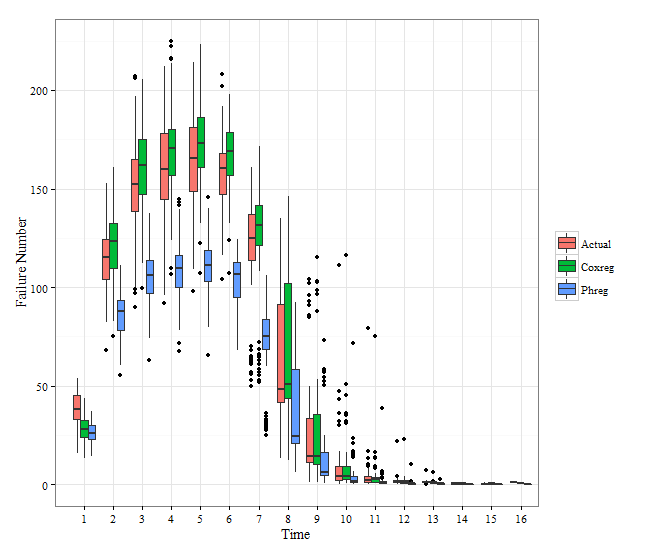
\includegraphics[width=3in]{Predev0.png}}
 	\quad
 	\subfloat[25\% Left Truncation]{\label{fig:left25}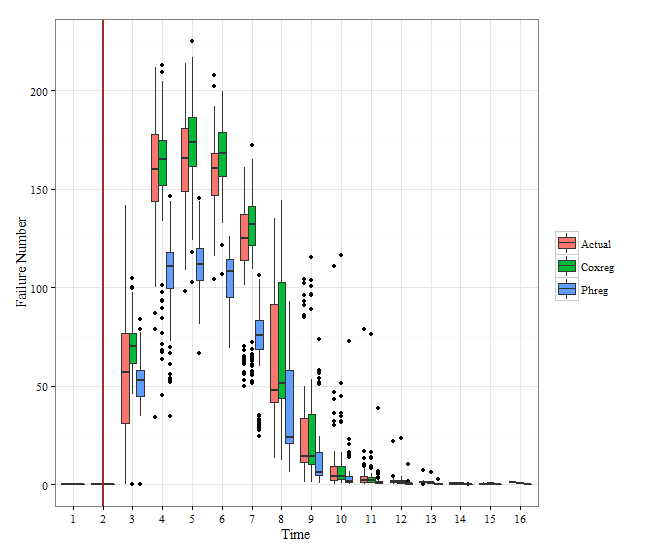
\includegraphics[width=3in]{Predev25.png}}
 	\quad
 	\subfloat[50\% Left Truncation]{\label{fig:left50}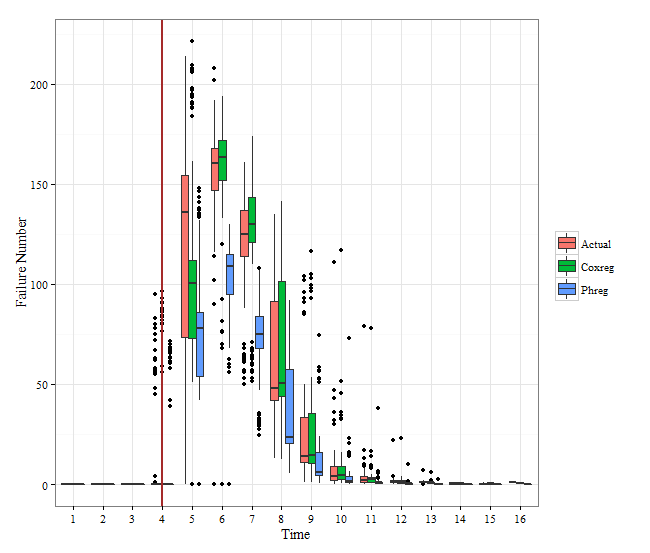
\includegraphics[width=3in]{Predev50.png}}
 	\quad
 	\subfloat[75\% Left Truncation]{\label{fig:left75}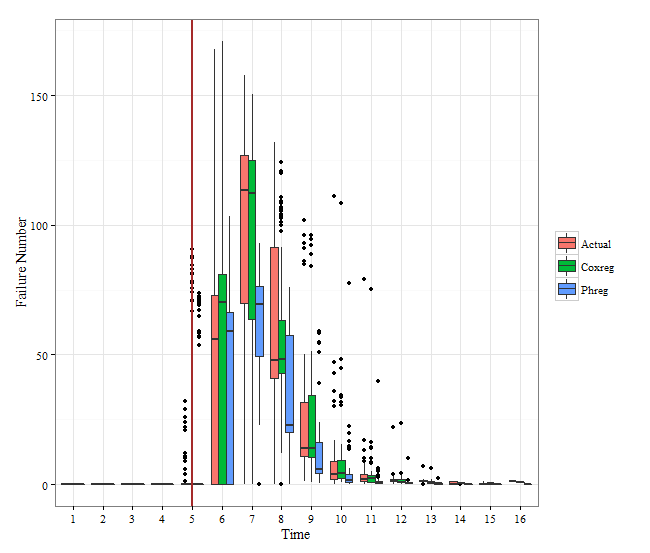
\includegraphics[width=3in]{Predev75.png}}
 	\caption{Left Truncation Simulation Results: Comparison of Actual vs. Cox PH and Parametric PH with EV baseline Predicted Failure Number}
 	\label{fig:lefttruncation}
 \end{figure}
Figure \ref{fig:leftbase} compares the non-parametric estimates of the baseline from the Cox PH model with two parametric proportional hazards fits estimated using $\tt eha$ \citep{eha}.  The first parametric fit is properly specified and assumes a  Weibull distribution as in the prior simulations.  The second fit assumes that data follow a type-I extreme value distribution[CHECK MANUAL ON THIS]. Unlike the simulation of Section \ref{rightcensor:sim2} the duration of non-parametric baseline estimates are not limited by the four left truncation proportions.  Both Weibull and Cox PH fits overlap with the variability of the Cox baselines showing increased variability with amount of truncation.  EV based fits all significantly underestimate the cumulative hazard indicating a potential risk of parametric modelling.  However, it is interesting to note that the EV fits converge slightly with increasing amounts of truncation.  This is a consequence of extreme-value theory and the theory of exceedances; more information about this phenomenon can be found in \citet{coles2001}.

Figure \ref{fig:lefttruncation} focuses on the number of
events predicted by the models.  Here 2000 events are generated using the protocol of this section. Both parametric and nonparametric models are fit to the data and this procedure is repeated 100 times. The red vertical line is the average left truncation time across the simulations for each truncation percentage.  Using each model, the expected number of failures is then predicted for each 1 unit time interval and compared to the observed number of failures.  Boxplots indicate the range of observed values across the 100 replications. The non-parametric Cox PH model tends to slightly overestimate the number of events in each interval indicating that baseline estimation is not affected by the left truncation.  The overestimation can be explained by the convention used to compute the survival probability over each interval.  The baseline survival function is stepwise decreasing and probabilities are based on the estimate at the most recent previous failure.  This slightly overestimates the failure for each each individual and in aggregate produces the observed overestimates.
Matching parametric estimates are generated using a PH model with extreme value (EV) baseline instead of the true Weibull model.  The underestimation of the baselines by the EV fit shown in Figure \ref{fig:leftbase} lead to drastic under-predictions of the number of events.


%Therefore, accurate estimation of coefficients and the baseline are two key factors impacts the perdition of the events of the Cox PH model. The simulation test shows that the Cox PH model can accurately estimates the coefficients when events number is at least 1000 even with high proportion of censor and left truncation. The baseline is another key factor to predict the number of events. The prediction will be accurate if the parametric distribution of the baseline is known or identify the correctly. Otherwise, a wrong baseline can also deteriorate the prediction. Compared to parametric baselines, a non-parametric baseline is more robust. However, it still needs enough number of events with curtain long period to get a smoothed and long baseline to predict accurately.



Simulations were performed to better understand the effects of truncation and censoring bias on predictions.

In the situations considered, we found that, if sample size are large enough, in particular if they exceeded 250 events, all parameter estimates showed very little bias under both parametric and semi-parametric models.  If samples were small, regression coefficients were slightly overestimated in both types of models.  For data sets with small numbers of events due to heavy right censoring, parametric models tend to overestimate both shape and scale both leading to an underestimate of the baseline.  Although the impact of right censoring on the non-parametric baseline is not directly quantified, Figure \ref{fig:rightdiff} suggests that baseline estimates are often smaller than the parametric versions and become more variable near the maximum lifetime.  Simulations show similar impacts of left truncation on covariate and baseline effects.  A major difference is that the length of the non-parametric baseline is potentially less limited due to the lack of censoring time.  This may not be relevant in real world data, which has both effects.

 Although this study has more than 50\% right censoring and an unknown proportion of left truncated cases, it still has more than 1000 retirement events, many with long duration (around 50 years length). Based on the simulation, we expect the Cox model to provide very accurate estimates of covariate effects in this case and highly accurate baseline estimates for most employees, particularly those with age less than 70.


\cite{}%
%With respect to prediction of retirement, because the s
%
%As a consequence, it is hard to accurately predict the employee turnover for a company just formed recently, or when the employee population characteristic changed, due to high proportion of censor and lack of events.



% The simulation is used to examine Cox PH model predictive performance with right censor and left truncation. The simulated lifetime data is generated based on the Weibull distribution. %The hazarld function for Weibull regression model with shape parameter $\alpha$, scale parameter $\lambda$, and variable $X$ is shown in equation \ref{eq:weibul}, given $h_0=\alpha(\lambda)^\alpha t^{\alpha-1}$:
 %\begin{equation} \label{eq:weibul}
 %\begin{split}% to allgin the equation
 %h(t|X) & =h_0(t)exp(\beta X) \\
 %         &=\alpha (\lambda (exp(\beta X)^{\frac{1}{\alpha}})^\alpha t^{\alpha-1} \\
 %         &=\alpha(\tilde{\lambda} )^\alpha t^{\alpha-1}
 %\end{split}
 %\end{equation}
 %where, $\tilde{\lambda}=\lambda (exp(\beta X)^{\frac{1}{\alpha}}$.
% The simulation can be described as follows. The sample size was n=100, 300, 500, 1000, and 4000, with one variable $X$, named Age, which follows uniform distribution with parameter $a$ $(a=22)$ and $b$ $(b=70)$. Only one variable age is used in simulation process to make the estimation procedure simple and close to real world. The coefficient $\beta_{age}$ is taken $-0.025$ and $\beta_0=1.5$.
%Then, the survival time $T$ is random generated for each observation based on Weibull distribution with shape parameter $\alpha$ and scale parameter $\lambda$, where $\alpha=1.5$ and $\lambda=exp(-0.025age+\beta_0)^{\frac{1}{\alpha}}$.

% The simulation is performed on right censoring and left truncation separately, in order to observe the effects for different bias.
% For right censor simulation, two simulation procedure are conducted with different start points. First, the start point for all the observations are equal to 0, and stop point is equal to the survival time $t_i$ for ith observation where $T=(t_1, t_2, \ldots, t_n)$. After that, the censor time $C$ is equal to first quarter, median, third quarter, and maximum of the survival time, respectively, to get 75\%, 50\%, 25\% and 0\% censor proportions. When the survival time $t_i$ for ith observation is not greater than the censor time ($c_i$), the stop point is survival time $t_i$ and censor variable $\delta_i$ is 1. When survival time $t_i$ for ith observation is greater than censor time ($c_i$), the stop point is change to censor time ($c_i$) and censor variable $\delta_i$ is 0. The second right censor simulation procedure is to set the start points $S$ to follow uniform distribution from 0 to 10, representing the observations (employees) start at various time points within 10 years study window. The stop point is equal to the summation of start point and survival time: $S+T$. The censor time is a cutoff point ($C$) identified by R to get fix number of censor proportion (25\%, 50\%, and 75\%).  When the survival time $t_i$ for ith observation is not greater than the censor time ($c_i$), the stop point is survival time $t_i$ and censor variable $\delta_i$ is 1. The stop points are set to censor time $C$ for the observations with the stop points $S+T$ being great than censor time $C$, the survival time is reset to $C-S$, and censor variable $\delta_i$ is 0. Otherwise, the other observations with stop point being less than the censor time remain the same and the censor variable $\delta_i$ is 1. For the second simulation, there are 4000 observations are generated. Because some observations occur after the cutoff point (censor time) and the sample size are various for different censor proportion, only 400 are randomly selected with 75\%, 50\%, 25\% and 0\% censor proportions to keep the sample size same. The start point and the stop point are dependent variable in the cox regression model. $\delta$ is censor variable.
%
% For left truncation simulation, the start point $U$ is generated as uniform distribution with $a=0$ and $b=max(T)$ which indicates an observation start randomly from time 0 to time $max(T)$. The stop point $S$ is $U+T$. The histogram is generated for $S$. The truncation time $L$ is set as 0, first quarter, median, and third quarter of $S$, respectively, to get 0\%, 25\%, 50\%, and 75\% truncation proportions. When start point $u_i$ for ith observation is less than truncation time $l_i$, the start point is reset as truncation time $l_i$. When start point $u_i$ for ith observation is not less than truncation time $l_i$, the start point does not change ($u_i$). In left truncation, the censor variable $\delta$ for all the observations are equal 1. For right censor and left truncation simulation,  the Cox regression models are modeled by "coxreg" and "phreg" function in eha package. The coxreg function is the regular cox regression modeling procedure to generate coefficient estimates and a non-parametric baseline.  The phreg funcation is using parametric distribution like Weibull, Extrem value (EV) to estimate the baseline. The "phreg" function performs Cox PH model and also provides a parametric baseline hazards estimation \citep{brostrom2012}. The phreg function is used to compare the non-parametric with parametric baseline and to demonstrate the prediction when the parametric baseline is not right.
% Total predicted failure number is calculated as shown in equation \ref{eq:prob} and \ref {eq:expturnover}. The actual and predicted failure number are compared to show right censor and left truncation's impacts on the coefficient and baseline estimation .
%
% %accelarate model%
% \subsection{Right censor and left truncation simulation results}
% % 1. right censor start 0 results shows in table 1a
% % 2. start different results shows in table 2 and figure 2 with different baseline and prediction number
% %    younger company has shorter baseline hard to predict beyond the baseline max time.
% % 3. left truncation simulation results shows in table 1 and figure 4&5
% % 4. shows the baseline using wrong parametric distribution (wrong) what is going on.
% The right censoring simulation results are shown in the left part of Table \ref{tab:rightcensor} which all the observations start at the same time 0. The events in the second column of the table are the actual total failure events simulated without considering censoring, which is $n=100, 200, 500, 1000, 2000, \text{and } 4000$. The number of events in the dataset applying to the Cox model are reduced due to the right censoring, which is equal to $events=\sum_{i=0}^{n}{\delta_i}$. The values in the other column are the average value of 100 replications for Cox PH model coefficient and baseline parameter estimates based on Weibull distribution using phreg. The simulation results show censoring proportion and the number of events are two influential factors for the coefficient estimation. The model overestimates the coefficients of age, $\lambda, \text{ and } \alpha$, when the dataset has high proportion of censoring. For example, when 75\% of the data are censored with only 25 events, the estimates for three parameters are 0.028, 4.043, and 1.564, respectively, which are the highest among all the estimates. As the event number increasing, the estimation is approaching to the actual value. For example, the estimation of age, $\lambda, \text{ and } \alpha$ are close to 0.025, 2.7, and 1.5, respectively, after the number of event is at least 500.
% The predicted events in the sixth column is the total predicted failure number calculated by applying the coefficient estimates and the non-parametric baseline from Cox PH models into the dataset without considering censoring. The predicted events using censoring models are all lower than the actual total failure number, but close to the number of events after censoring. For example, the number of predicted events is 24.84 when using the estimates of Cox PH model with 75\% censoring to calculate the dataset with 100 events, which is close to 25. The prediction is less than the actual dataset, because the baseline is lack of information for the events after censored time. The baseline does not include hazards or survival probability information for the long life time observation, because the baseline just captures the events before the censor time and the observation with long life time are censored in this simulation. As a result, there is no failure probability for long life time observation.
%




 %\begin{figure}[h!]
% 	\centering
% 	\subfloat[No right censor ]{\label{fig:rightno}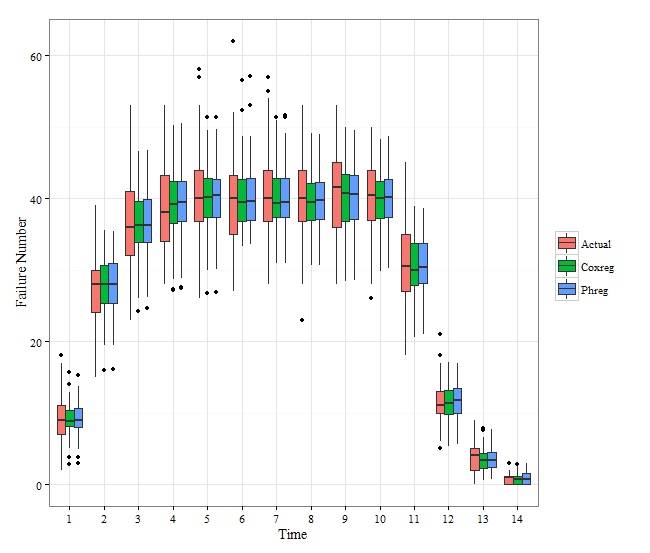
\includegraphics[width=3in]{right0.png}}
% 	\quad
% 	\subfloat[25\% right censor]{\label{fig:right25}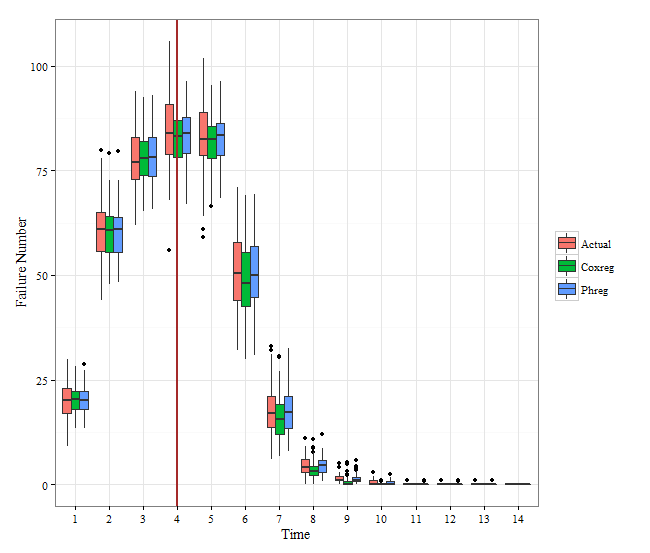
\includegraphics[width=3in]{right25.png}}
% 	\quad
% 	\subfloat[50\% right censor ]{\label{fig:right50}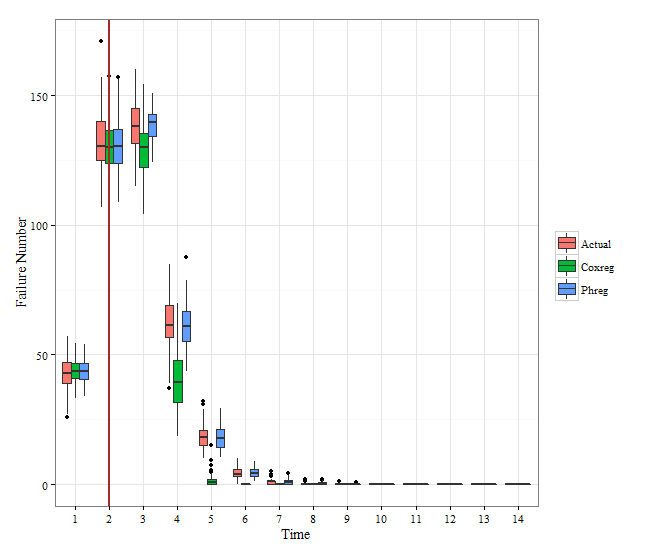
\includegraphics[width=3in]{right50.png}}
% 	\quad
% 	\subfloat[75\% right censor]{\label{fig:right75}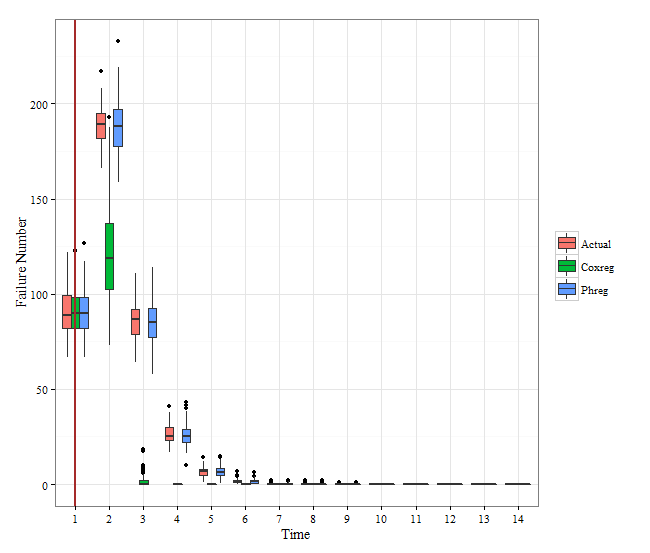
\includegraphics[width=3in]{right75.png}}
% 	\caption{Right censor simulation results: actual vs. predicted failure number}
% 	\label{fig:rightpred}
% \end{figure}

 % % % % % % % % % % % % % % % % % % % % % % % % %
 % % % %Left truncation result % % % % % % % % % %
 % % % % % % % % % % % % % % % % % % % % % % % % %


 % 1- include the name of the package in the Results sections.
 % 2 - redo with results averaged over 100 data sets.
 % 3 - explain concerns about censoring in our data.  About 50 % censored.  Large amount of truncation.
 % 4) - Baseline can be highly variable in the extremes leading to poor
 % 5) Figures and discussion of coefficients and baseline estimates and impact on predictions.
 % 6) Problems with PH in predictive modelling.  Truncation needs PH (is there another method)
 %



%put this graphic in policy discussion part


% Table generated by Excel2LaTeX from sheet 'summary'
%\begin{landscape}


% Please add the following required packages to your document preamble:

%\end{landscape}
 % Table generated by Excel2LaTeX from sheet 'Sheet6' %accelarate model%
%%%%%%%%%%%%%%%%%%%%%%%%%%%%%%%%%%%%%%%
%%%%% Commentted on 12/14/2015%%%%%%%%%%%%
%%%%%%%%%%%%%%%%%%%%%%%%%%%%%%%%%%%%%%%
%\subsection{Right censor and left truncation simulation results}
%% 1. right censor start 0 results shows in table 1a
%% 2. start different results shows in table 2 and figure 2 with different baseline and prediction number
%%    younger company has shorter baseline hard to predict beyond the baseline max time.
%% 3. left truncation simulation results shows in table 1 and figure 4&5
%% 4. shows the baseline using wrong parametric distribution (wrong) what is going on.
%The right censoring simulation results are shown in the left part of Table \ref{tab:rightcensor} which all the observations start at the same time 0. The events in the second column of the table are the actual total failure events simulated without considering censoring, which is $n=100, 200, 500, 1000, 2000, \text{and } 4000$. The number of events in the dataset applying to the Cox model are reduced due to the right censoring, which is equal to $events=\sum_{i=0}^{n}{\delta_i}$. The values in the other column are the average value of 100 replications for Cox PH model coefficient and baseline parameter estimates based on Weibull distribution using phreg. The simulation results show censoring proportion and the number of events are two influential factors for the coefficient estimation. The model overestimates the coefficients of age, $\lambda, \text{ and } \alpha$, when the dataset has high proportion of censoring. For example, when 75\% of the data are censored with only 25 events, the estimates for three parameters are 0.028, 4.043, and 1.564, respectively, which are the highest among all the estimates. As the event number increasing, the estimation is approaching to the actual value. For example, the estimation of age, $\lambda, \text{ and } \alpha$ are close to 0.025, 2.7, and 1.5, respectively, after the number of event is at least 500.
%The predicted events in the sixth column is the total predicted failure number calculated by applying the coefficient estimates and the non-parametric baseline from Cox PH models into the dataset without considering censoring. The predicted events using censoring models are all lower than the actual total failure number, but close to the number of events after censoring. For example, the number of predicted events is 24.84 when using the estimates of Cox PH model with 75\% censoring to calculate the dataset with 100 events, which is close to 25. The prediction is less than the actual dataset, because the baseline is lack of information for the events after censored time. The baseline does not include hazards or survival probability information for the long life time observation, because the baseline just captures the events before the censor time and the observation with long life time are censored in this simulation. As a result, there is no failure probability for long life time observation.
%% Please add the following required packages to your document preamble:
%% \usepackage{booktabs}
%\begin{table}[]
%	\renewcommand{\arraystretch}{1.5}
%	\scriptsize %table fond
%	\centering
%	\caption{Right censoring and left truncation simulation statistics}
%	\begin{tabular}{@{}C{1.8cm}lllll||C{1.8cm}lllll@{}}
%		\toprule
%		\multicolumn{6}{c}{Right Censor}  & \multicolumn{6}{c}{Left Truncation}                \\ \midrule
%		Right Censor Proportion & Events & $\beta_{coxreg}$ & $\beta_{phreg}$ & Scale & Shape & Left Truncation Propotion & Events &$\beta_{coxreg}$ & $\beta_{phreg}$ & Scale & Shape \\
%		\midrule
%		0\%                     & 100    & 0.026        & 0.027       & 2.931 & 1.509 & 0\%                       & 100    & 0.027        & 0.027       & 2.865 & 1.534 \\
%		25\%                    & 100    & 0.027        & 0.027       & 2.962 & 1.527 & 25\%                      & 75     & 0.027        & 0.027       & 2.917 & 1.546 \\
%		50\%                    & 100    & 0.028        & 0.028       & 3.237 & 1.530 & 50\%                      & 50     & 0.027        & 0.027       & 2.899 & 1.577 \\
%		75\%                    & 100    & 0.028        & 0.028       & 4.043 & 1.564 & 75\%                      & 25     & 0.029        & 0.029       & 3.280 & 1.757 \\
%		0\%                     & 200    & 0.026        & 0.026       & 2.841 & 1.508 & 0\%                       & 199    & 0.025        & 0.025       & 2.777 & 1.506 \\
%		25\%                    & 200    & 0.026        & 0.026       & 2.856 & 1.513 & 25\%                      & 150    & 0.025        & 0.025       & 2.756 & 1.515 \\
%		50\%                    & 200    & 0.026        & 0.026       & 2.925 & 1.527 & 50\%                      & 100    & 0.025        & 0.025       & 2.825 & 1.532 \\
%		75\%                    & 200    & 0.026        & 0.026       & 3.167 & 1.540 & 75\%                      & 50     & 0.026        & 0.026       & 2.927 & 1.572 \\
%		0\%                     & 500    & 0.025        & 0.025       & 2.731 & 1.500 & 0\%                       & 500    & 0.025        & 0.025       & 2.732 & 1.509 \\
%		25\%                    & 500    & 0.025        & 0.025       & 2.718 & 1.508 & 25\%                      & 375    & 0.025        & 0.025       & 2.737 & 1.514 \\
%		50\%                    & 500    & 0.025        & 0.025       & 2.744 & 1.514 & 50\%                      & 250    & 0.026        & 0.026       & 2.778 & 1.514 \\
%		75\%                    & 500    & 0.025        & 0.025       & 2.787 & 1.525 & 75\%                      & 125    & 0.026        & 0.026       & 2.835 & 1.547 \\
%		0\%                     & 1000   & 0.025        & 0.025       & 2.748 & 1.509 & 0\%                       & 999    & 0.025        & 0.025       & 2.710 & 1.504 \\
%		25\%                    & 1000   & 0.025        & 0.025       & 2.747 & 1.512 & 25\%                      & 750    & 0.025        & 0.025       & 2.709 & 1.504 \\
%		50\%                    & 1000   & 0.025        & 0.025       & 2.748 & 1.514 & 50\%                      & 500    & 0.025        & 0.025       & 2.715 & 1.506 \\
%		75\%                    & 1000   & 0.026        & 0.026       & 2.844 & 1.509 & 75\%                      & 250    & 0.025        & 0.025       & 2.694 & 1.524 \\
%		0\%                     & 2000   & 0.025        & 0.025       & 2.714 & 1.502 & 0\%                       & 2000   & 0.025        & 0.025       & 2.740 & 1.503 \\
%		25\%                    & 2000   & 0.025        & 0.025       & 2.713 & 1.503 & 25\%                      & 1500   & 0.025        & 0.025       & 2.731 & 1.502 \\
%		50\%                    & 2000   & 0.025        & 0.025       & 2.742 & 1.500 & 50\%                      & 1000   & 0.025        & 0.025       & 2.724 & 1.503 \\
%		75\%                    & 2000   & 0.025        & 0.025       & 2.733 & 1.502 & 75\%                      & 500    & 0.025        & 0.025       & 2.718 & 1.508 \\
%		0\%                     & 4000   & 0.025        & 0.025       & 2.719 & 1.504 & 0\%                       & 3999   & 0.025        & 0.025       & 2.720 & 1.500 \\
%		25\%                    & 4000   & 0.025        & 0.025       & 2.718 & 1.505 & 25\%                      & 3000   & 0.025        & 0.025       & 2.722 & 1.501 \\
%		50\%                    & 4000   & 0.025        & 0.025       & 2.724 & 1.503 & 50\%                      & 2000   & 0.025        & 0.025       & 2.710 & 1.502 \\
%		75\%                    & 4000   & 0.025        & 0.025       & 2.729 & 1.513 & 75\%                      & 1000   & 0.025        & 0.025       & 2.703 & 1.503 \\ \bottomrule
%	\end{tabular}
%    \label{tab:rightcensor}%
%\end{table}
%
%
%
%\begin{table}[htbp]
%	\renewcommand{\arraystretch}{1.5}
%	%\scriptsize %table fond
%	\centering
%	\caption{Right censor simulation results by various start time}
%	\begin{tabular}{ccccccc}
%		\toprule
%    	\multicolumn{1}{c}{\multirow{2}{1.5cm}{Censor proportion}}  & \multirow{2}[4]{*}{Events} & \multicolumn{3}{c}{Variable Estimaties} & \multicolumn{2}{c}{Predicted Events} \\ \cline{3-7}
%		     &       & Age   & $\lambda$ & $\alpha$ & "coxreg" & "phreg" \\
%		\midrule
%		0\%   & 400   & 0.025 & 2.694 & 1.508 & 398.52 & 400.44 \\
%		25\%  & 400   & 0.026 & 2.802 & 1.518 & 394.24 & 401.72 \\
%		50\%  & 400   & 0.026 & 2.828 & 1.514 & 340.73 & 398.51 \\
%		75\%  & 400   & 0.025 & 2.821 & 1.518 & 215.92 & 400.80 \\
%		\bottomrule
%	\end{tabular}%
%	\label{tab:right2}%
%\end{table}%
%
%
%\begin{figure}[h!]
%	\centering
%	\subfloat[No right censor ]{\label{fig:baseno}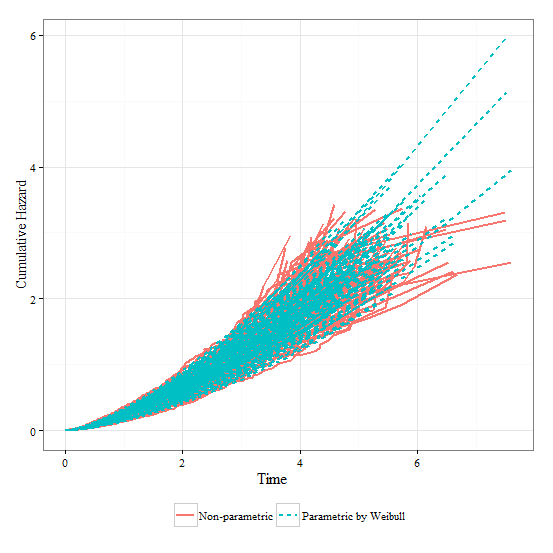
\includegraphics[width=3in]{base0.png}}
%	\quad
%	\subfloat[25\% right censor]{\label{fig:base25}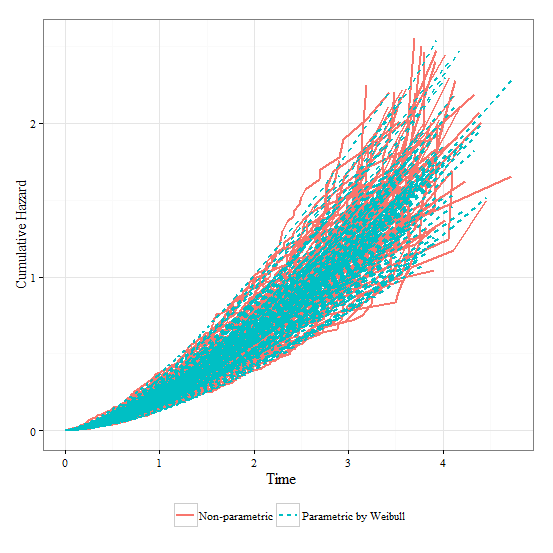
\includegraphics[width=3in]{base25.png}}
%	\quad
%	\subfloat[50\% right censor ]{\label{fig:base50}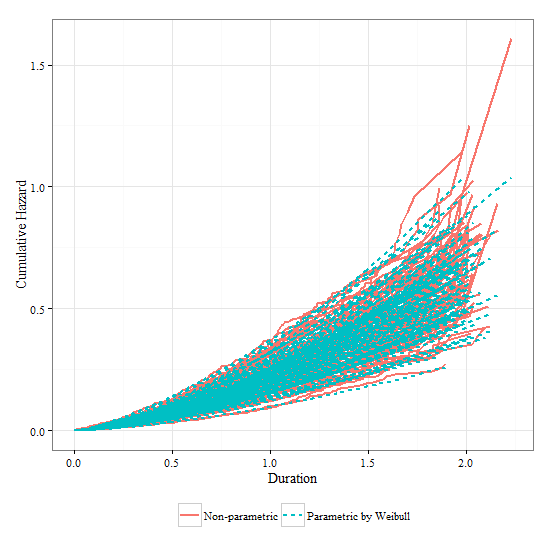
\includegraphics[width=3in]{base50.png}}
%	\quad
%	\subfloat[75\% right censor]{\label{fig:base75}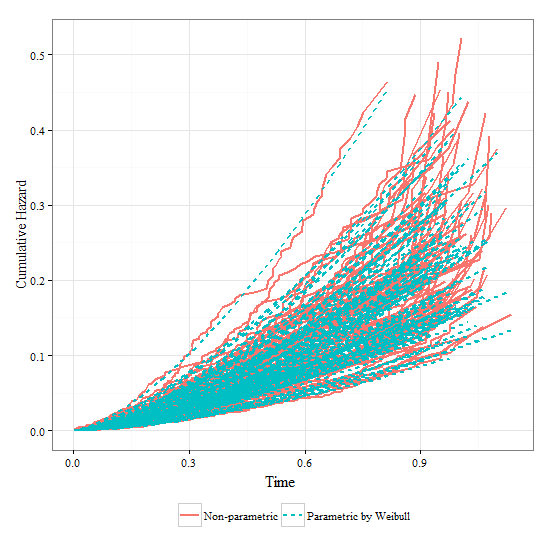
\includegraphics[width=3in]{base75.png}}
%	\caption{Baseline comparison by various censoring}
%	\label{fig:rightbase}
%\end{figure}
%
%\begin{figure}[h!]
%	\centering
%	\subfloat[No right censor ]{\label{fig:rightno}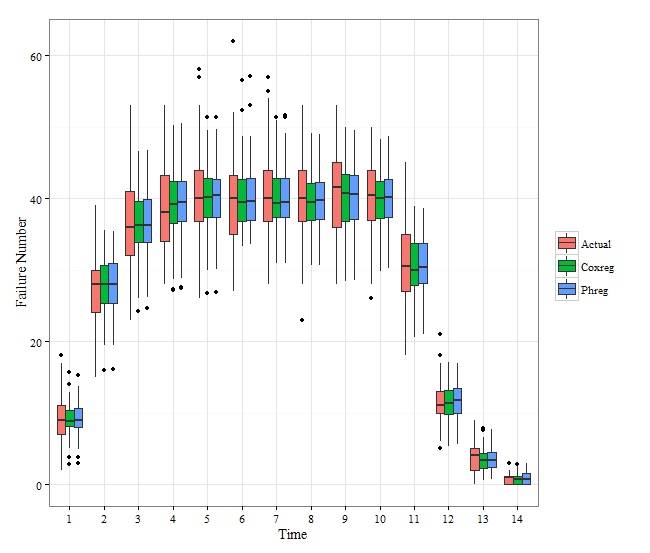
\includegraphics[width=3in]{right0.png}}
%	\quad
%	\subfloat[25\% right censor]{\label{fig:right25}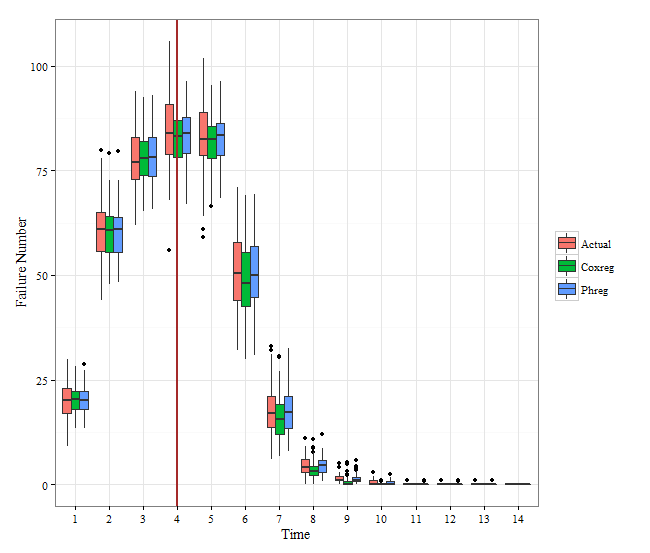
\includegraphics[width=3in]{right25.png}}
%	\quad
%	\subfloat[50\% right censor ]{\label{fig:right50}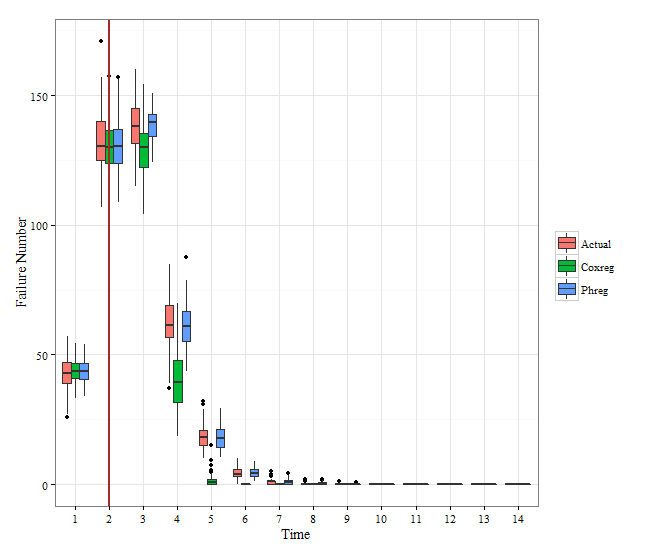
\includegraphics[width=3in]{right50.png}}
%	\quad
%	\subfloat[75\% right censor]{\label{fig:right75}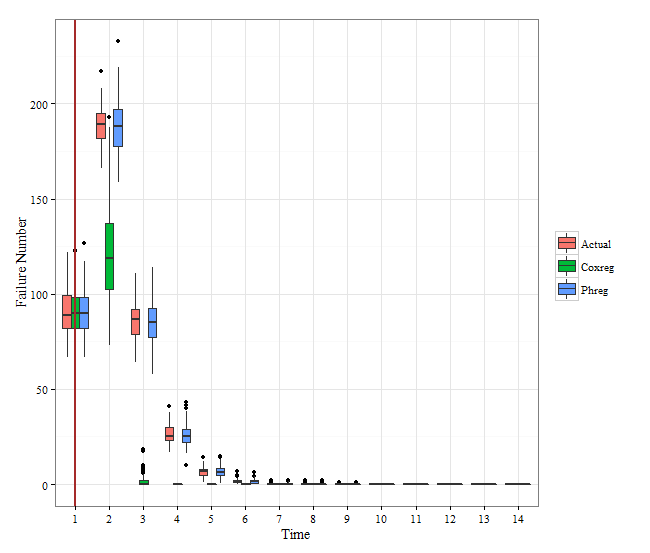
\includegraphics[width=3in]{right75.png}}
%	\caption{Right censor simulation results: actual vs. predicted failure number}
%	\label{fig:rightpred}
%\end{figure}
%
%To simulate the realistic situation, the second right censor simulation is conducted with randomly occurrence of the observations followed by uniform distribution. The results are shown in the table \ref{tab:right2}. The events without considering censoring are all equal to 400 for easy comparison. The predicted events include the prediction by non-parametric baselines using "coxreg" and by parametric baseline using "phreg" function Weibull distribution as baseline estimation. The estimation of age and $\alpha$ are all close to the simulated value (0.025 and 1.5). And the estimation of $\lambda$ are around 2.8. These indicate the right censoring does not impact the coefficients estimation. However, right censoring does impact the baseline function estimation for Cox PH model as shown in the figure \ref{fig:rightbase}. The red lines in the figure \ref{fig:rightbase} are the non-parametric baseline for 100 replications. And blue dash lines are the parametric baseline generated base on Weibull distribution for 100 replications, which represent the actual baseline. All these baselines are overlap together by various censoring, which indicates non-parametric baseline can capture the true parametric baseline. However, the duration of the non-parametric baseline is getting short by increasing the censoring proportion. As a result, the predicted number of events using non-parametric baseline is less than the actual failure number. However, it does not affect the prediction by using parametric baseline, which are all close to 400, because the parametric baseline is not limited by the baseline duration if the parameters are correctly estimated. The prediction by "coxreg" and "phreg" are plotted across time by box plot to compare to the actual failure values as shown in the figure \ref{fig:rightpred}. The vertical red line is the average value of censor time. The predicted number of events by "coxreg" are close to actual and the prediction by "phreg" before the censor time line. It is still close to actual after censor time line for the data with no censoring and with 25\% of censoring as shown in the figure \ref{fig:rightno} and \ref{fig:right25}, because of the long baseline duration. However, It drops down gradually after the censor time for the data with 50\% and 75\% of censoring as shown in figure \ref{fig:right50} and \ref{fig:right75}, because the baseline duration ends around censor time. This simulation clearly shows the limitation of Cox PH model with
%non-parametric baseline: it cannot accurate predict far beyond the duration of the longest events. Therefore, a baseline can be highly variable in the extremes leading to poor predictions. Although this simulates the real problem, the employee hiring time points are followed by uniform distribution in the real world.
%
%% % % % % % % % % % % % % % % % % % % % % % % % %
%% % % %Left truncation result % % % % % % % % % %
%% % % % % % % % % % % % % % % % % % % % % % % % %
%\begin{figure}[h!]
%	\centering
%	\subfloat[No left truncation]{\label{fig:ev0}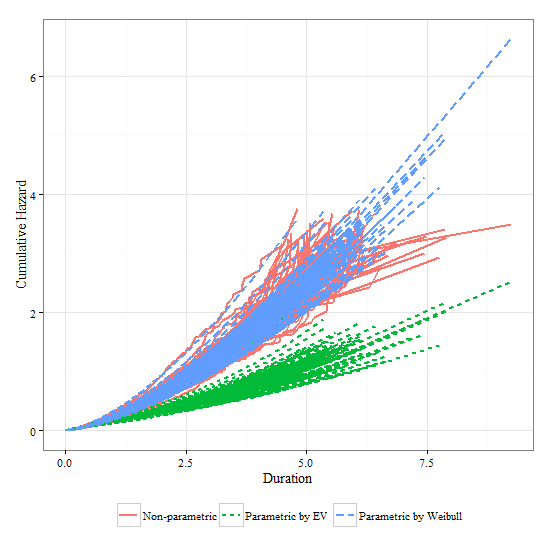
\includegraphics[width=3in]{EV0.png}}
%	\quad
%	\subfloat[25\% left truncation]{\label{fig:ev25}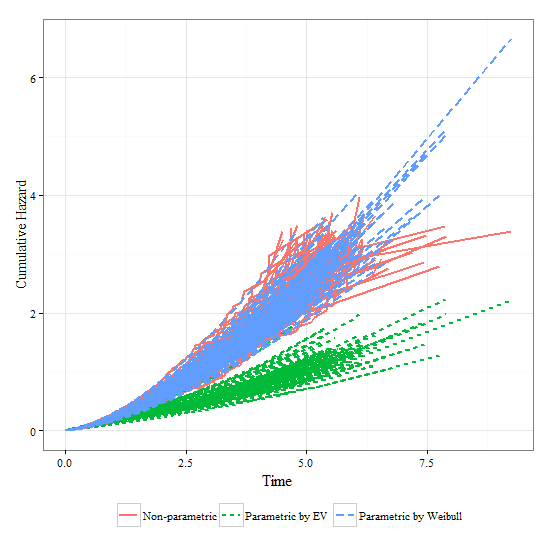
\includegraphics[width=3in]{EV25.png}}
%	\quad
%	\subfloat[50\% left truncation]{\label{fig:ev50}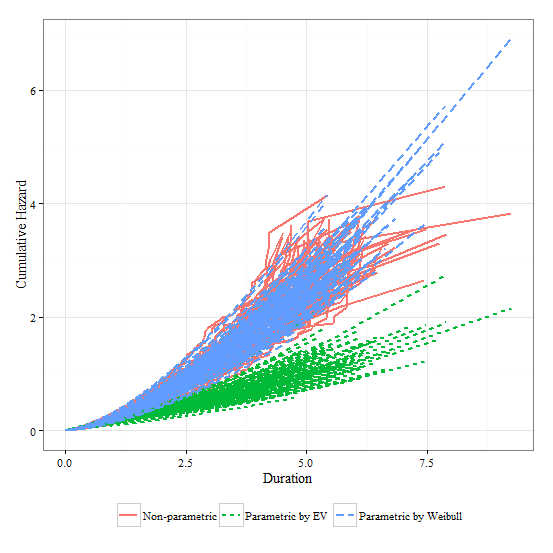
\includegraphics[width=3in]{EV50.png}}
%	\quad
%	\subfloat[75\% left truncation]{\label{fig:ev75}\includegraphics[width=3in]{EV75.png}}
%	\caption{Left truncation simulation results: Baseline Comparison}
%	\label{fig:leftbase}
%\end{figure}
%
%\begin{figure}[h!]
%	\centering
%	\subfloat[No left truncation]{\label{fig:leftno}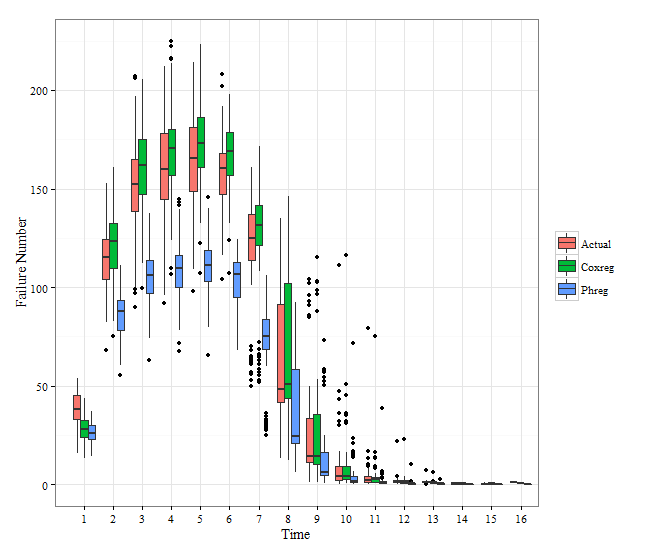
\includegraphics[width=3in]{Predev0.png}}
%	\quad
%	\subfloat[25\% left truncation]{\label{fig:left25}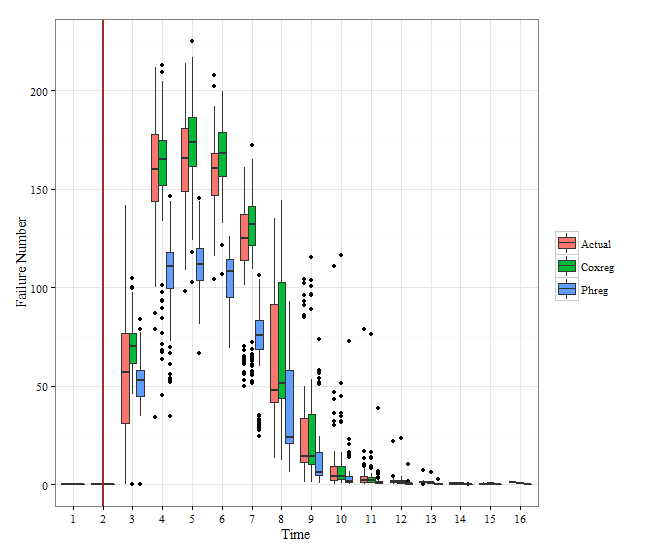
\includegraphics[width=3in]{Predev25.png}}
%	\quad
%	\subfloat[50\% left truncation]{\label{fig:left50}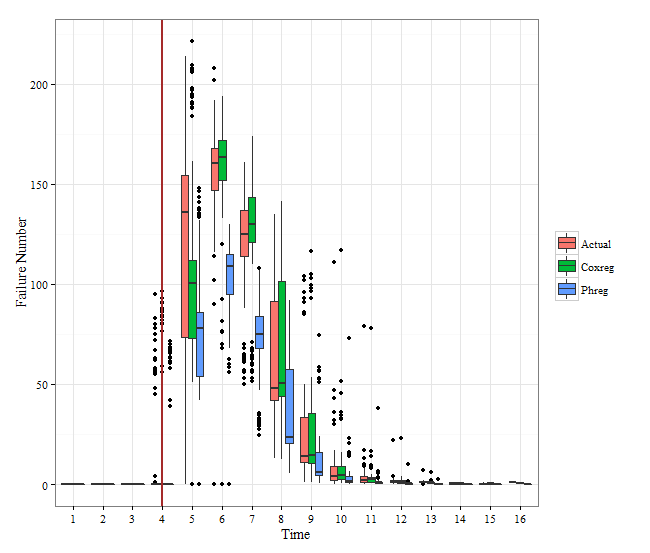
\includegraphics[width=3in]{Predev50.png}}
%	\quad
%	\subfloat[75\% left truncation]{\label{fig:left75}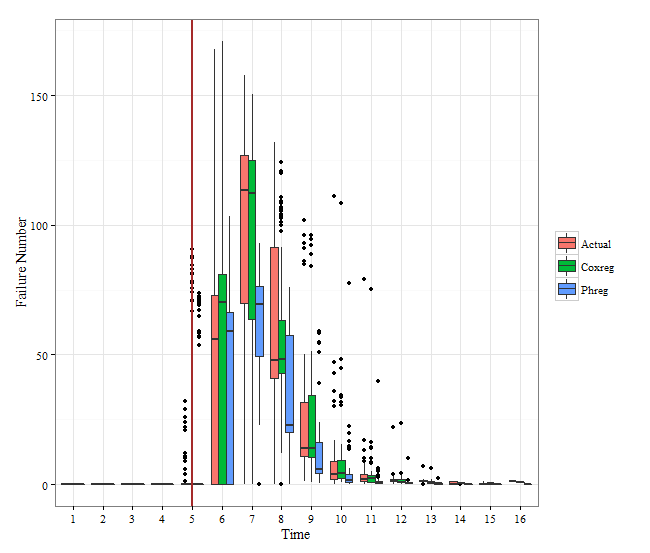
\includegraphics[width=3in]{Predev75.png}}
%	\caption{Left truncation simulation results: actual vs. predicted failure number}
%	\label{fig:lefttruncation}
%\end{figure}
%The results of the left truncation bias simulation statistics are shown in the right part of table \ref{tab:rightcensor}. All the values shown are the average value for coefficient estimate of age, and baseline parameter estimates of $\lambda$ and $\alpha$ by "phreg" Weibull distribution. The last column is the total predicted number of events using non-parametric baseline by "coxreg" function. Similar as the right censor simulation result, left truncation proportion and the number of events are two key factors for coefficients estimation. As table \ref{tab:rightcensor} shown, the coefficients are overestimated when the left truncation proportion is 75\% or the number of events are less than 200. However, increasing the number of events can offset (reduce) the left truncation effects. For example, the estimates for age and $\alpha$ are all close to simulated value, when the number of events is 1000 with 75\% truncation proportion. The predicted number of events is close to the actual one as shown the green and red box in the figure \ref{fig:lefttruncation}, which is the box plot of total 2000 events simulated with 100 replication by various proportion of left truncation. The red vertical line is the average of left truncation time. It is slightly overestimated using "coxreg" non-parametric baseline by four left truncation proportions, because the baseline estimation is not affected by the left truncation. The figure \ref{fig:leftbase} clear shows the duration of non-parametric baseline are the same for four left truncation proportion. It also shows the non-parametric baselines (red lines) are overlap with parametric baseline (blue dash lines).
%
%To further test how baseline estimation impacts on the prediction, another simulation is conducted accompanied with left truncation simulation. In the previous left truncations study, the parametric baseline using Extreme Value (EV) distribution is generated by "phreg" and predicted the number of events based on it shape and scale parameter estimation as shown in figure \ref{fig:leftbase}. Because the data is generated by Weibull distribution, the parametric baselines (green dash line) by EV are much lower than the other two baselines by all four left truncation proportions. The predicted number of events based on the EV baseline are also much lower than the actual number of events across the time as the blue box shown in the figure \ref{fig:lefttruncation}. This study shows the inaccuracy estimation of the baseline lead to poor prediction.
%
%Therefore, accurate estimation of coefficients and the baseline are two key factors impacts the perdition of the events of the Cox PH model. The simulation test shows that the Cox PH model can accurately estimates the coefficients when events number is at least 1000 even with high proportion of censor and left truncation. The baseline is another key factor to predict the number of events. The prediction will be accurate if the parametric distribution of the baseline is known or identify the correctly. Otherwise, a wrong baseline can also deteriorate the prediction. Compared to parametric baselines, a non-parametric baseline is more robust. However, it still needs enough number of events with curtain long period to get a smoothed and long baseline to predict accurately. As a result, it is hard to accurately predict the employee turnover for a company just formed recently, or when the employee population characteristic changed, due to high proportion of censor and lack of events. Although this study has more than 50\% right censor, it still has more than 3000 events with long duration (around 50 years length).
%
%
%
%
%
%
%% 1- include the name of the package in the Results sections.
%% 2 - redo with results averaged over 100 data sets.
%% 3 - explain concerns about censoring in our data.  About 50 % censored.  Large amount of truncation.
%% 4) - Baseline can be highly variable in the extremes leading to poor
%% 5) Figures and discussion of coefficients and baseline estimates and impact on predictions.
%% 6) Problems with PH in predictive modelling.  Truncation needs PH (is there another method)
%%
%
%% Table generated by Excel2LaTeX from sheet 'Sheet6'


\section{Results \& Analysis} \label{application}

The construction of predictive models for turnover involves consideration of several factors. Among the variables available for analysis, we must choose the set that offers the maximum predictive power, i.e. a model that includes variables that provide the best possible predictions on out of sample testing data sets and not simply on data used to train the model. We must also evaluate potential strengths and weaknesses of the baseline hazard estimate and its impact on prediction accuracy.  The bootstrap will be a useful tool in assessing uncertainty in model predictions. From the perspective of administration it will also be useful to contemplate the ERIP implications of the predictors found to have an impact on prediction.

\subsection{Descriptive Analysis}

As described in Section \ref{data.desc}, the current data provides five demographic and career history variables: PR (hourly, weekly, or monthly payroll), GENDER (M, F), DIV (ten levels of division), OC (crafts, engineers, general administrative, laborers, managers, administrative, operators, scientists, technicians), AGEH, and YCSH. Table \ref{tab:descriptive} provides marginal counts of the number of workers in the sample within each category.  We see that among occupation codes there are four large categories (C, E, M, \&P)  with over one thousand employees observed throughout the data sample, four medium sized groups with 500-700 employees (G, L, R, \&T), and one small group, S, with 208 employees.  Payroll data shows that the largest group is paid monthly, followed by hourly, and weekly.  In terms of gender, approximately 72\% of employees are male. Finally, divisions, while not fixed over the life of the employee, are distributed in a similar fashion to occupational codes with four larger groups and a number of smaller groups.
\begin{table}[htbp]
	\centering
	\scriptsize
	\renewcommand{\arraystretch}{1.5}
	\caption{Descriptive Statistics}
	\begin{tabular}{lrrlrr}
		\toprule
		\textbf{Variable}	& \multicolumn{1}{c}{\textbf{Count}} & \multicolumn{1}{c}{\textbf{N \%}}  &   \textbf{Variable}    & \multicolumn{1}{c}{\textbf{Count}} & \multicolumn{1}{c}{\textbf{N \%}} \\
		\midrule
		\textbf{OC} &       &       & \textbf{GENDER} &       &  \\
		C     & 1295  & 16.0\% & F     & 2296  & 28.4\% \\
		E     & 1361  & 16.8\% & M     & 5802  & 71.6\% \\
		G     & 574   & 7.1\% & \textbf{DIV} &       &  \\
		L     & 613   & 7.6\% & Div1 & 1542  & 19.0\% \\
		M     & 1178  & 14.5\% & Div2 & 751   & 9.3\% \\
		P     & 1621  & 20.0\% & Div3 & 1042  & 12.9\% \\
		R     & 595   & 7.3\% & Div4 & 369   & 4.6\% \\
		S     & 208   & 2.6\% & Div5 & 398   & 4.9\% \\
		T     & 652   & 8.1\% & Div6 & 1199  & 14.8\% \\
		Missing & 1     & 0.0\% & Div7 & 302   & 3.8\% \\
		\textbf{PR} &  &   & Div8 & 823   & 10.2\% \\
		Hourly & 2503  & 30.9\% & Div9 & 404   & 5.0\% \\
		Monthly & 4369  & 54.0\% & Div10 & 1268  & 15.7\% \\
		Weekly & 1226  & 15.1\% &       &       &  \\
		\bottomrule
	\end{tabular}%
	\label{tab:descriptive}%
\end{table}%

\begin{table}[htbp]
	\centering
	\scriptsize
	\caption{Discriptive Statistics 2}
	\begin{tabular}{lrrrrrrr}
		\toprule
		& Count & Mean  & Median & Mode  & Minimum & Maximum & Std. Deviation \\
		\midrule
		\multicolumn{1}{l}{Age at Retire} & 1757  & 59.72 & 60.00 & 62.00 & 49.00 & 84.00 & 4.56 \\
		\multicolumn{1}{l}{Years of Service at Retire} & 1757  & 29.72 & 30.90 & 30.06 & 0.05  & 55.68 & 7.74 \\
		\multicolumn{1}{l}{Points at Retire} & 1757  & 89.44 & 88.67 & 85.47 & 51.05 & 136.66 & 9.15 \\
		\bottomrule
	\end{tabular}%
	\label{tab:descrip2}%
\end{table}%

\begin{figure}[h!]
	\centering
	\subfloat[]{\label{fig:age}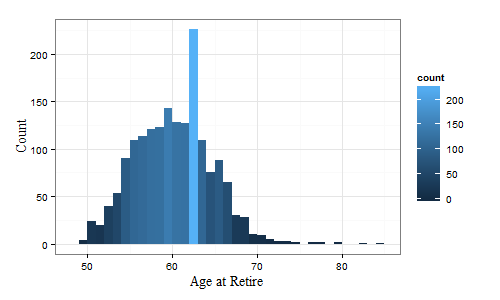
\includegraphics[width=0.5\textwidth]{Agetdhist.png}}
	\subfloat[]{\label{fig:point}\includegraphics[width=0.5\textwidth]{pointdhist.png}}
	%\subfloat[Hazard function]{\label{fig:Hazard}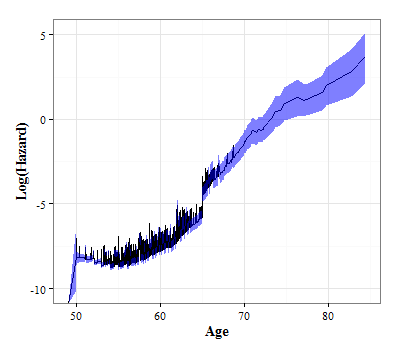
\includegraphics[width=0.35\textwidth]{loghazard.png}}
	\caption{Histogram of Age and Point at Retire}
	\label{fig:hist}
\end{figure}

Beyond these demographic and career factors, our models also include behavioral variables derived from policy requirements for retirement and early retirement incentives that occur throughout the observation period. Histograms of retirement age and accumulated pension points are shown in Figure \ref{fig:hist}. The histogram of retirement age is right skewed and shows an anomalous spike at age equals 62 which is the mode.  We find that 79\% of the employees that retired at 62 also reached or exceeded 85 points.
[COMMENTS:WHY IS THIS SUCH A POPULAR AGE?  MEDICARE, SOCIAL SECURITY? ]
The average retirement age is 59.72 demonstrating that many individuals retire before 62 and most before age 70. In terms of points accrued at time of retirement, recall that points are the sum of years of service plus current age, we see an irregular distribution with the vast majority retiring with point totals in the range of 85 to 100. Relatively few elect to take a reduced pension and retire with diminished benefits with points below 85. Again we see that 85 points is the mode indicating that retiring immediately after become fully vested in the pension is a popular choice.

\subsection{Models for Retirement without External Economic Variables}
Section \ref{sec:modelchoice} discussed two potential response variables that are suitable for time until turnover models, age and years of service from hire.  Because of the existence of time varying covariates and the need for a baseline estimate to facilitate predictions, we chose to model age at retirement arranging the data in a counting process format (SAS will only estimate the baseline if the counting process formulation is used).

%1) Need counting process form for time varying covariates.
%2) Need counting process form to estimate the baseline from CoxPh Model.
%3) Need


%put this graphic in policy discussion part


% Table generated by Excel2LaTeX from sheet 'summary'
%\begin{landscape}
\begin{table}[htbp]
	\centering
	\scriptsize
	\caption{Models Statistics for Retirement}
	\renewcommand{\arraystretch}{1.5}
	\begin{tabular}{lL{3.5cm}lllllrrrr}
		\toprule
		\multicolumn{1}{c}{\textbf{No.}}  &\multicolumn{1}{c}{	\textbf{Model}}&  \multicolumn{1}{c}{\textbf{LR}}    &\multicolumn{1}{c}{\textbf{AIC}}   & \multicolumn{1}{c}{\textbf{SBC}}   & \multicolumn{1}{c}{\textbf{\begin{tabular}[c]{@{}c@{}}Pred. \\ MAPE\end{tabular}}} & \multicolumn{1}{c}{\textbf{\begin{tabular}[c]{@{}c@{}}Holdout \\ MAPE\end{tabular}}} &\multicolumn{1}{c}{\textbf{\begin{tabular}[c]{@{}c@{}}Pred. \\ $G^2$\end{tabular}}} & \multicolumn{1}{c}{\textbf{\begin{tabular}[c]{@{}c@{}}Holdout \\ $G^2$\end{tabular}}}  \\
		\midrule
		1 & DIV GENDER PR OC YCSH AGEH & 1194.3 & 19271.3  & 19377.3 &  39.44 & 56.78 & 381.77 & 85.19 \\
		2 & DIV OC YCSH AGEH & 1193.8  & 19269.8 & 19370.5 &  39.45 & 56.84 & 381.92 & 85.29 \\
		3 & DIV ERIP YCSH AGEH & 1451.6  & 18998  & 19061.6 &  25.91 & 15.51 & 128.75 & 2.64 \\
		4 & DIV ERIP YCSH AGEH OC & 1469.92  & 18995.7  & 19101.7 &   25.91 & 15.24 & 129.47 & 2.56 \\
	% DIV ERIP YCSH AGEH and Strata on OC  & 1426.34 & 14602.1 & 13199.8 & 14602.1 & 13263.4 &  43.45 & 87.92 & 186.89 & 50.00 \\
		%9 models by OC & N/A   & N/A   & N/A   & N/A      &    24.62 & 3.40  & 117.9 & 0.26 \\
		5 & DIV ERIP YCSH AGEH  P85 & 1826.95  & 18624.6  & 18693.6 &  25.59 & 19.04 & 109.17 & 3.40 \\
		6 &DIV ERIP YCSH AGEH  P85 P85*A65 & 1873.69  & 18579.9  & 18654.1 &  25.38 & 7.97  & 111.55 & 0.79 \\
		7 &DIV ERIP YCSH AGEH P85 P85*A65 P85*ERIP & 1881.02  & 18574.6  & 18654.0 & 25.42 & 4.20  & 112.27 & 0.81 \\
	%	Logistic  regression  & 4103.91 & 13618.4 & 9556.53 & 13627.3 & 9752.1 &  28.20 & 31.73 & 232.84 & 117.38 \\
		8 &Time series  & N/A     & N/A     & N/A   &   11.17 & 34.38 & 32.10 & 8.54 \\
		\bottomrule
	\end{tabular}%
	\label{tab:modelstats}%
\end{table}%

Extensive model selection using a variety of metrics including log-likelihood, AIC, BIC, and out of sample predictive scoring (MAPE and $G^2$) was then applied to identify key predictive factors in the model as shown in Table \ref{tab:modelstats}. %This is likely due to the fact that age 62 is the earliest age for a person to receive social security retirement benefit.
The first four models listed are all standard Cox PH models with various sets of explanatory variables.  Among these four, the third model offers the lowest BIC value, 19061, while the fourth has the lowest AIC, 18,996 indicating these two models are the best of this subset.  Overall, both models perform almost identically on MAPE and holdout MAPE which is error when the model is used on data from years 2011 and 2012 which was not used to train the model. $G^2$ and holdout $G^2$ were also nearly identical.  From this perspective, the variable OC seems to provide very little predictive impact.   Model 5 uses the same variables as 1 - 4 but uses OC as a stratification variable meaning that we create a separate baseline for each job classification variable.  Creating multiple baselines for subgroups makes the model significantly more complex leading to a huge reduction in log likelihood and traditional model fit but providing very poor predictive and holdout fits due to the significant overfitting of the data.[THIS DOESN'T MAKE SENSE DUE TO THE PREVIOUS FINDING-OC IS NOT A GOOD TARGET-NEED TO DECIDE HOW TO REWORK THIS].

Models 5-7 build on model 3 and add various interaction terms.  Here again we find models 6 and 7 being roughly equivalent with the more complex model having a smaller AIC and holdout MAPE, and very slightly higher predicted $G^2$ and predicted MAPE.  In the end, we chose to explore the more complex model 7 due to interest in interpreting the interacting model coefficients.[MAYBE NOT A GOOD REASON, CHECK IF SBC IS RIGHT]

Finally, for comparison purposes we include a time series prediction model discussed in \cite{zhu2015}.  This forecast is based on a four component time series decomposition model, which includes terms for trend, cycle, seasonality, and irregularity.  This model is fit to monthly aggregate retirement counts for the period of November 2000 to December 2010 based on the same data used here. The model produces an aggregate forecast by month leading to a very accurate MAPE on the training data but much poorer performance out of sample. It does not provide accurate forecasts by occupational code (OC) due to the small individual samples for each subgroup. Furthermore, it is not possible to include the effects of other explanatory facors in this model.

%why did we choose the ones we did

%The time series model is really good, is it a fair comparison

%Any other discrepancies?

Excluding aggregate economic factors, the optimal modelling variables for the prediction of age at retirement include DIV, YCSH, and AGEH.  In addition, based on our understanding of the covenants and parameters of the retirement program we found several additional variables that increase the predictive power of the model. These include ERIP, P85, A65*P85, an interaction term that moderates the impact of the P85 effect after the individual has exceeded 65 years of age, and  ERIP*P85, an interaction term that moderates the impact of the P85 effect while the ERIP is in place.  These variables were introduced in Section \ref{data.desc}.

Table \ref{tab:paraest.} describes the fit parameters and hazard ratios.  As noted above, we did not find that gender, occupational code and payroll category were statistically significant predictors indicating that employees' gender, job types, and payroll status are not associated with choice of retirement age conditional on the other variables in the model.
\begin{table}[htbp]
	\centering
	\scriptsize
	\renewcommand{\arraystretch}{1.5}
	\caption{Parameter Estimates for Retirement Models}
	\begin{threeparttable}
		\begin{tabular}{llL{2.5cm}L{1.5cm}L{2.5cm}L{1.5cm}}
			\toprule
			&       & \multicolumn{2}{c}{\textbf{Model W/O External Variable}} & \multicolumn{2}{c}{\textbf{Model with Real Earnings}} \\
			\hline
			Parameter &   Label & Parameter (Standard Error) & Hazard Ratio & Parameter (Standard Error) & Hazard Ratio \\
			\midrule
			%			division & dir2  & -0.965(0.179)***\tnote{1} & 0.381 &-1.025(0.177)*** & 0.359 \\
			%			division & dir3  & -0.241(0.112)* & 0.786 & -0.246(0.111)* & 0.782 \\
			%			division & dir4  & 0.078(0.195) & 1.081 & -0.039(0.195) & 0.962 \\
			%			division & dir5  & -0.131(0.190) & 0.877 & -0.246(0.190) & 0.782 \\
			%			division & dir6  & 2.136(0.095)*** & 8.463 & 2.252(0.095)*** & 9.511 \\
			%			division & dir7  & 2.435(0.129)*** & 11.418 & 2.437(0.129)*** & 11.437 \\
			%			division & dir8  & 0.864(0.106)*** & 2.373 & 0.816(0.106)*** & 2.261 \\
			%			division & dir9  & -3.023(0.581)*** & 0.049 & -2.774(0.504)*** & 0.062 \\
			%			division & dir10 & 0.793(0.093)*** & 2.211 & 0.709(0.093)*** & 2.031 \\
			%			YCSH  &       & 0.019(0.004)*** & 1.019 & 0.043(0.004)*** & 1.044 \\
			%			ERIP & 1     & 0.859(0.169)*** & .     & 0.942(0.109)*** & . \\
			%			AGEH &       & -0.172(0.013)*** & 0.842 & -0.187(0.013)*** & 0.829 \\
			%			P85   & 1     & 1.435(0.091)*** & .     & 0.682(0.072)*** & . \\
			%			A65*P85 & 1     & -1.610(0.206)*** & .     & -0.662(0.177)*** & . \\
			%			ERIP*P85 & 1     & 0.469(0.179)** & .     & 0.600(0.130)*** & . \\
			DIV & Div2  & -0.965 (0.179)*** & 0.381 & -0.969 (0.177)*** & 0.38 \\
			DIV & Div3  & -0.241 (0.112)* & 0.786 & -0.242 (0.111)* & 0.785 \\
			DIV & Div4  & 0.078 (0.195) & 1.081 & 0.013 (0.195) & 1.013 \\
			DIV & Div5  & -0.131 (0.19) & 0.877 & -0.216 (0.19) & 0.806 \\
			DIV & Div6  & 2.136 (0.095)*** & 8.463 & 2.261 (0.093)*** & 9.594 \\
			DIV & Div7  & 2.435 (0.129)*** & 11.418 & 2.515 (0.128) & 12.363 \\
			DIV & Div8  & 0.864 (0.106)*** & 2.373 & 0.855 (0.106)*** & 2.352 \\
			DIV & Div9  & -3.023 (0.581)*** & 0.049 & -2.731 (0.504)*** & 0.065 \\
			DIV & Div10 & 0.793 (0.093)*** & 2.211 & 0.726 (0.093)*** & 2.068 \\
			YCSH  & 1     & 0.019 (0.004)*** & 1.019 & 0.023 (0.004)*** & 1.023 \\
			ERIP  &       & 0.859 (0.169)*** & .     & 0.489 (0.133)*** & . \\
			AGEH  &       & -0.172 (0.013)*** & 0.842 & -0.193 (0.014)*** & 0.825 \\
			P85   & 1     & 1.435 (0.091)*** & .     & 0.756 (0.073)*** & . \\
			P85*A65 & 1     & -1.61 (0.206)*** & .     & -1.019 (0.197)*** & . \\
			ERIP*P85 & 1     & 0.469 (0.179)** & .     & 0.506 (0.141)*** & . \\
			Real Earnings &       &       &       & 0.013 (0.001)*** & 1.013 \\
			\bottomrule
		\end{tabular}%
		\begin{tablenotes}
			\item[1] * denotes $P<0.05$, ** denotes $P<0.01$, and *** denotes $P<0.001$.
		\end{tablenotes}
	\end{threeparttable}
	\label{tab:paraest.}%
\end{table}%	
P85 is an indicator that a person is eligible for maximum retirement benefits and naturally this has a strong impact on the probability that a person will retire.  From a quantitative point of view, with all other factors held constant, for those that achieve 85 points before the age of 65, the hazard ratio is $e^{1.44} = 4.22$ meaning that the hazard of retirement becomes 4.22 times more likely.  While not surprising, this quantification is important in predicting individual and aggregate retirement and reflects the modal spike observed in the histogram in Figure \ref{fig:point}.

An alternative eligibility criteria for retirement occurs when individuals exceed an age of 65 years and so we would anticipate the hazard increasing at this point in an employees career.  Because the response variable in our model is age, the impact of this 65 year effect is included in the baseline hazard, which should increase after this point.  Figure \ref{fig:basepred} shows the baseline survival and cumulative hazard function for a standard case. Independent of the P85 effect, we see a further steep increase in the cumulative hazard/decrease in survival between age 62 and 65. By including an interaction between the indicators of age greater than 65 and points greater than 85, A65*P85, we can estimate how the impact of reaching 85 points changes when a person exceeds regular retirement age.  In this case, the interaction term is estimated at -1.61 indicating a diminishing effect on the P85 criteria to $e^{1.44-1.61} =0.84$.  In addition, as can be seen from the trend of the cumulative hazard, the baseline hazard seems to return lower levels.  Hence, those that exceed both criteria actually have a reduced hazard of retiring over those have only met the age 65 criteria.  It seems that the fact that the individual remains on the job after hitting both criteria indicates a diminished intention to retire.

According to our model, retirement can also be influenced by an employee's age at time of hire and their years of service at the time of hiring.  The coefficient estimate for age is -0.17. As the reference age is 45.49, this means that the hazard ratio for retirement of an employee that started working at age 46.49 is $e^{-.017}=.84$ indicating a 16\% drop in hazard for each additional year later that an employee started. The employee's survival probability at any time, $t$, can be computed as $S(t)^{1.19} = (S(t)^{e^{0.17}})$ when age at hire is one year below 45.49,  where $S(t)$ is the baseline survival probability for a reference employee of average age at the time of hiring. Moving in the other direction, an employee's survival probability is $S(t)^{0.84}=(S(t)^{e^{-0.17}})$ for a one year increase beyond 45.49 in the employee's starting age. Together, this implies that at any given retirement age, the employee who starts earlier is more likely to retire because they have more years of service and are closer to vesting full benefits (85 points) than an equivalent employee who starts working at an older age. Similarly, the employee's years of service at hire show a positive estimate (0.019) with a hazard ratio (1.019) indicating that each year of service at hire beyond the population average of 2.75 is associated with an approximately 2\% increase in the hazard of retirement.  This leads to a survival probability $S(t)^{0.98}$ for a one year decrease in the reference years of service at time of hiring.  On the other hand, the survival probability is $S(t)^{1.019}$ for an employee with one year of service above average at the time of hire. Together, both age at hire and YCSH effects reflect the intuitive fact that, all else being equal, an employee who has more years of service and therefore is closer to full vesting is more likely to retire.  What is non-intuitive about this finding is that while one might suspect that the effects should be of similar magnitude, we actually see that the effect of one year difference in age seems to have about 8 times the impact that one year of previous service does on the hazard of retirement.

\begin{figure}[h!]
	\centering
	\subfloat[Retirement Rate]{\label{fig:ratio}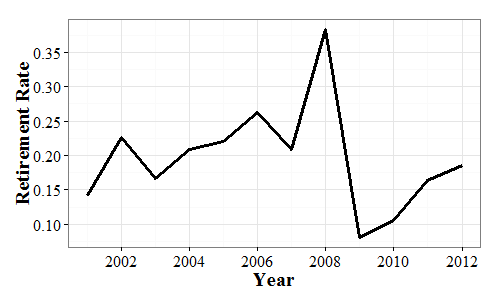
\includegraphics[width=0.5\textwidth]{reratio.png}}
	\subfloat[Prediction w/o Variable ERIP]{\label{fig:nopolicy}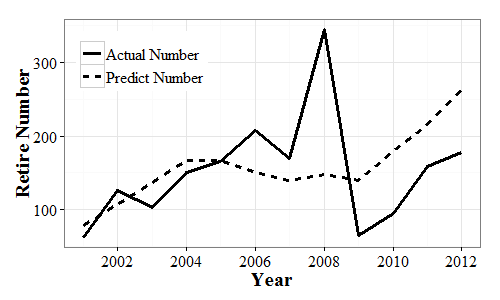
\includegraphics[width=0.5\textwidth]{nopolicy.png}}
	\caption{Retirement Rate and Prediction Plot}
	\label{fig:rerate}
\end{figure}

In the fiscal year 2008, the employer in this study created a temporary early retirement incentive program (ERIP). The response window for this option was 3 months although the specific details beyond this are unknown. In order to deal with the increased level of retirement during this period we include a time dependent indicator variable for each employee that indicates their age when this program was in effect.  The coefficient for this indicator was 0.86 leading to a hazard ratio of $e^{.86} = 2.21$ which indicates that, on average, an individuals hazard of retirement increased by almost 2.2 times during this period.  If more information were known about the requirements or targets of this ERIP, a more case specific estimate may be possible.  The effect of the ERIP is considerable as indicated by the huge uptick in events in 2008; see Figure \ref{fig:predict}.  If this one-time effect were not included in the model it may bias the other estimates parameters considerably.
	
As a further step, we test the ERIP effect on the employees who are eligible for getting a pension, i.e. points greater than 85.  After adding an interaction term between ERIP and the indicator that a person exceeds 85 points, the hazard ratio for the ERIP increases substantially to 15.85 from 2.21, more than seven times the basic ERIP effect. In contrast, employees that were eligible only for partial retirement, an interaction between ERIP and indicator variables that employees achieve only 65 or 75 points, were not statistically significant.

The DIV variable was also a significant predictor.  For analysis, the baseline level was chosen arbitrarily as division 1 so that its hazard rate is determined by the baseline.  Relative to this baseline, divisions 6 and 7 have very high hazard ratios, 8.363 and 11.405 respectively, which indicates, other factors being equal, that the employees in division 6 and 7 are much more likely to retire at any age than those from division 1.  Conversely, division 9 has a hazard ratio of $e^{-3.023} = .049$ indicating that individuals within this group have 1/20 the hazard of group 1.  This may indicate that the division is new and contains younger employees.  In general, differences in retirement rates could be caused by differences in age demographics, departmental and job functions, or departmental leadership.

The baseline survival function and log hazard function are shown in Figure \ref{fig:basepred}. The survival probability is 1 before age 49 as shown in Figure \ref{fig:Surv}, which indicates that no employees retire before this age. The survival probability starts to slowly decease from age 50 to age 62. By age 62 the survival probability has decreased by nearly 25\%, which indicates that 75\% of employees retire at an age greater than 62 years assuming that they are at average or baseline levels for other factors included in the model.  The slope of the survival function decreases sharply at this point indicating the increased retirement rates for workers between age 62 and 65.  After age 65 the probability drops off even further as most of the remaining population retires by age 68 or 69. Accompanying the survival function is the log of the cumulative hazard ratio.  Again, the steep rise in the cumulative hazard between age 62 and 65 indicates the increased retirement activity during this period.  Afterward the cumulative hazard levels off, indicating a drop in the instantaneous hazard rate at these future points.
\begin{figure}[h!]
	\centering
	\subfloat[Survival Function]{\label{fig:Surv}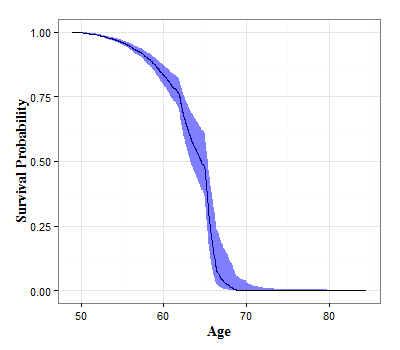
\includegraphics[width=0.5\textwidth]{Surv.png}}
	\subfloat[Cumulative Hazard]{\label{fig:Cumh}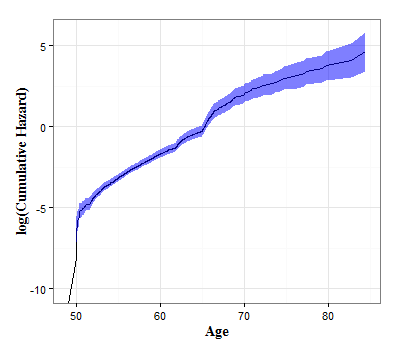
\includegraphics[width=0.5\textwidth]{logcum.png}}
	%\subfloat[Hazard function]{\label{fig:Hazard}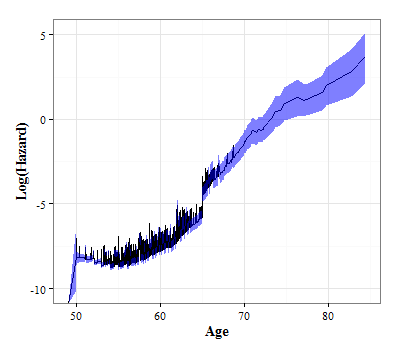
\includegraphics[width=0.35\textwidth]{loghazard.png}}
	\caption{Baselines with 95\% Confident Intervals}
	\label{fig:basepred}
\end{figure}


%% Table generated by Excel2LaTeX from sheet 'Sheet2'
%\begin{table}[htbp]
%	\centering
%	\scriptsize
%	\renewcommand{\arraystretch}{1.5}
%	\caption{Parameter Estimates for Models}
%	\begin{threeparttable}
%		\begin{tabular}{llL{2.5cm}L{1.5cm}L{2.5cm}L{1.5cm}}
%			\toprule
%			&       & \multicolumn{2}{c}{\textbf{Period Model}} & \multicolumn{2}{c}{\textbf{Yearly model}} \\
%			\hline
%			Parameter &   Label & Parameter (Standard Error) & Hazard Ratio & Parameter (Standard Error) & Hazard Ratio \\
%			\midrule
%			division & dir2  & -0.965(0.179)***\tnote{1} & 0.381 &-1.025(0.177)*** & 0.359 \\
%			division & dir3  & -0.241(0.112)* & 0.786 & -0.246(0.111)* & 0.782 \\
%			division & dir4  & 0.078(0.195) & 1.081 & -0.039(0.195) & 0.962 \\
%			division & dir5  & -0.131(0.190) & 0.877 & -0.246(0.190) & 0.782 \\
%			division & dir6  & 2.136(0.095)*** & 8.463 & 2.252(0.095)*** & 9.511 \\
%			division & dir7  & 2.435(0.129)*** & 11.418 & 2.437(0.129)*** & 11.437 \\
%			division & dir8  & 0.864(0.106)*** & 2.373 & 0.816(0.106)*** & 2.261 \\
%			division & dir9  & -3.023(0.581)*** & 0.049 & -2.774(0.504)*** & 0.062 \\
%			division & dir10 & 0.793(0.093)*** & 2.211 & 0.709(0.093)*** & 2.031 \\
%			YCSH  &       & 0.019(0.004)*** & 1.019 & 0.043(0.004)*** & 1.044 \\
%			ERIP & 1     & 0.859(0.169)*** & .     & 0.942(0.109)*** & . \\
%			AGEH &       & -0.172(0.013)*** & 0.842 & -0.187(0.013)*** & 0.829 \\
%			P85   & 1     & 1.435(0.091)*** & .     & 0.682(0.072)*** & . \\
%			A65*P85 & 1     & -1.610(0.206)*** & .     & -0.662(0.177)*** & . \\
%			ERIP*P85 & 1     & 0.469(0.179)** & .     & 0.600(0.130)*** & . \\
%			\bottomrule
%		\end{tabular}%
%		\begin{tablenotes}
%			\item[1] * denotes $P<0.05$, ** denotes $P<0.01$, and *** denotes $P<0.001$.
%		\end{tablenotes}
%		
%	\end{threeparttable}
%	\label{tab:paraest.}%
%\end{table}%

		
\begin{figure}[h!]
	\centering
	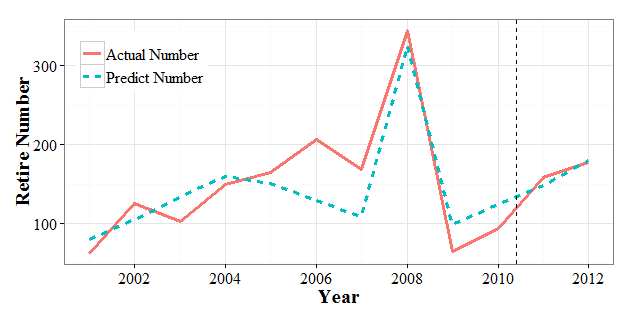
\includegraphics[width=5in]{retire2.png}
	\caption{Retirement Forecasting}
	\label{fig:predict}	
	
\end{figure}

\begin{table}[h!]
	\centering
	\scriptsize
	\smallskip
	\caption{Retirement Predictions by Occupational Code (OC) without External Variables}
	\begin{threeparttable}
		\begin{tabular}{cL{1.2cm}L{1.2cm}L{1.2cm}L{1.2cm}L{1.2cm}L{1.2cm}L{1.2cm}L{1.2cm}L{1.2cm}l}
			\toprule
			Year  &  Crafts & Engineers& General Admin. & Laborers& Managers& Prof. Admin.& Operators& Scientists& Technicians& Total \\
			\midrule
			%			2001  & 23\tnote{1} (16)\tnote{2} & 12 (10) & 4 (1) & 6 (5) & 11 (14) & 10 (9) & 8 (2) & 2 (1) & 4 (4) & 80 (62) \\
			%			2002  & 31 (29) & 15 (16) & 5 (15) & 7 (11) & 15 (26) & 13 (18) & 11 (6) & 2 (1) & 6 (4) & 105 (126) \\
			%			2003  & 37 (26) & 19 (13) & 6 (5) & 9 (6) & 17 (21) & 18 (13) & 16 (15) & 4 (2) & 8 (2) & 134 (103) \\
			%			2004  & 44 (32) & 23 (23) & 8 (9) & 11 (7) & 21 (30) & 23 (25) & 16 (15) & 4 (3) & 10 (6) & 160 (150) \\
			%			2005  & 40 (39) & 24 (17) & 8 (13) & 9 (7) & 20 (27) & 24 (31) & 12 (15) & 3 (4) & 11 (12) & 151 (165) \\
			%			2006  & 31 (58) & 20 (29) & 6 (10) & 8 (9) & 19 (32) & 25 (37) & 9 (13) & 2 (4) & 9 (15) & 129 (207) \\
			%			2007  & 19 (44) & 14 (25) & 7 (9) & 6 (9) & 18 (26) & 27 (40) & 8 (6) & 3 (4) & 7 (6) & 109 (169) \\
			%			2008  & 54 (71) & 30 (33) & 20 (20) & 22 (12) & 64 (63) & 80 (84) & 26 (32) & 6 (7) & 22 (23) & 324 (345) \\
			%			2009  & 16 (14) & 9 (6) & 7 (3) & 7 (7) & 21 (8) & 25 (10) & 8 (11) & 1 (1) & 5 (5) & 99 (65) \\
			%			2010  & 19 (19) & 11 (17) & 9 (1) & 7 (8) & 28 (23) & 34 (16) & 8 (4) & 1 (3) & 7 (3) & 124 (94) \\
			%			2011  & 22 (36) & 13 (25) & 11 (8) & 9 (9) & 34 (27) & 40 (34) & 9 (5) & 2 (1) & 8 (13) & 148 (158) \\
			%			2012  & 24 (29) & 16 (23) & 14 (11) & 12 (10) & 41 (46) & 49 (36) & 12 (4) & 3 (2) & 9 (16) & 180 (177) \\
			2001  & 23\tnote{1} (16)\tnote{2} & 12 (10) & 4 (1) & 6 (5) & 11 (14) & 11 (9) & 8 (2) & 2 (1) & 4 (4) & 81 (62) \\
			2002  & 31 (29) & 15 (16) & 5 (15) & 7 (11) & 15 (26) & 13 (18) & 11 (6) & 2 (1) & 6 (4) & 105 (126) \\
			2003  & 37 (26) & 18 (13) & 6 (5) & 9 (6) & 17 (21) & 18 (13) & 16 (15) & 4 (2) & 8 (2) & 133 (103) \\
			2004  & 43 (32) & 23 (23) & 8 (9) & 11 (7) & 21 (30) & 23 (25) & 15 (15) & 4 (3) & 10 (6) & 158 (150) \\
			2005  & 40 (39) & 24 (17) & 8 (13) & 9 (7) & 20 (27) & 24 (31) & 12 (15) & 3 (4) & 11 (12) & 151 (165) \\
			2006  & 31 (58) & 20 (29) & 6 (10) & 8 (9) & 19 (32) & 25 (37) & 9 (13) & 2 (4) & 9 (15) & 129 (207) \\
			2007  & 19 (44) & 14 (25) & 7 (9) & 6 (9) & 18 (26) & 27 (40) & 8 (6) & 3 (4) & 7 (6) & 109 (169) \\
			2008  & 55 (71) & 30 (33) & 19 (20) & 22 (12) & 64 (63) & 79 (84) & 27 (32) & 6 (7) & 21 (23) & 323 (345) \\
			2009  & 16 (14) & 9 (6) & 7 (3) & 7 (7) & 20 (8) & 25 (10) & 8 (11) & 1 (1) & 5 (5) & 98 (65) \\
			2010  & 18 (19) & 11 (17) & 9 (1) & 7 (8) & 28 (23) & 34 (16) & 8 (4) & 1 (3) & 7 (3) & 123 (94) \\
			2011  & 22 (36) & 13 (25) & 11 (8) & 9 (9) & 34 (27) & 40 (34) & 9 (5) & 2 (1) & 8 (13) & 148 (158) \\
			2012  & 24 (29) & 16 (23) & 14 (11) & 12 (10) & 41 (46) & 49 (36) & 12 (4) & 3 (2) & 9 (16) & 180 (177) \\
			
			\bottomrule
		\end{tabular}%
		\begin{tablenotes}
			\item[1] the number before the parentheses is predicted retirement number.
			\item[2] the number inside the parentheses is actual retirement number.
		\end{tablenotes}
		
	\end{threeparttable}
	\label{tab:cocscode}
\end{table}


%% Table generated by Excel2LaTeX from sheet 'Sheet4'
%\begin{table}[h!]
%	\centering
%	\scriptsize
%	\caption{Prediction by division}
%	\begin{threeparttable}
%		\begin{tabular}{clllllllllll}
%			\toprule
%			Year  & \multicolumn{1}{c}{DIV1} & \multicolumn{1}{c}{DIV2} & \multicolumn{1}{c}{DIV3} & \multicolumn{1}{c}{DIV4} & \multicolumn{1}{c}{DIV5} & \multicolumn{1}{c}{DIV6} & \multicolumn{1}{c}{DIV7} & \multicolumn{1}{c}{DIV8} & \multicolumn{1}{c}{DIV9} & \multicolumn{1}{c}{DIV10} \\
%			\midrule
%			%			2001  & 3\tnote{1} (0)\tnote{2} & 0 (0) & 1 (0) & 0 (0) & 0 (0) & 56 (43) & 11 (2) & 5 (10) & 0 (0) & 5 (7) \\
%			%			2002  & 4 (0) & 0 (0) & 2 (0) & 0 (0) & 0 (0) & 72 (54) & 14 (2) & 6 (38) & 0 (0) & 8 (32) \\
%			%			2003  & 6 (0) & 1 (0) & 2 (0) & 0 (0) & 0 (0) & 89 (44) & 19 (7) & 6 (18) & 0 (0) & 9 (34) \\
%			%			2004  & 9 (0) & 1 (0) & 4 (0) & 1 (0) & 1 (0) & 101 (96) & 26 (29) & 7 (13) & 0 (0) & 10 (12) \\
%			%			2005  & 13 (0) & 1 (0) & 5 (0) & 1 (0) & 1 (0) & 88 (114) & 20 (26) & 8 (18) & 0 (0) & 14 (7) \\
%			%			2006  & 19 (34) & 2 (0) & 8 (0) & 2 (5) & 2 (3) & 58 (105) & 12 (32) & 9 (12) & 0 (0) & 17 (16) \\
%			%			2007  & 23 (59) & 3 (0) & 12 (5) & 3 (7) & 3 (9) & 26 (53) & 3 (10) & 12 (6) & 0 (0) & 24 (20) \\
%			%			2008  & 85 (97) & 14 (23) & 51 (79) & 11 (11) & 12 (13) & 16 (16) & 0 (0) & 45 (24) & 1 (0) & 86 (82) \\
%			%			2009  & 27 (17) & 5 (4) & 15 (21) & 4 (3) & 4 (3) & 0 (0) & 0 (0) & 16 (4) & 0 (0) & 27 (13) \\
%			%			2010  & 32 (25) & 7 (10) & 19 (20) & 6 (4) & 6 (4) & 0 (0) & 0 (0) & 23 (6) & 1 (4) & 32 (21) \\
%			%			2011  & 38 (51) & 9 (15) & 23 (25) & 7 (8) & 7 (9) & 0 (0) & 0 (0) & 28 (12) & 1 (15) & 34 (23) \\
%			%			2012  & 42 (36) & 13 (15) & 30 (15) & 9 (3) & 10 (3) & 0 (0) & 0 (0) & 32 (14) & 1 (8) & 41 (15) \\
%			2001  & 3\tnote{1} (0)\tnote{2} & 0 (0) & 1 (0) & 0 (0) & 0 (0) & 57 (43) & 11 (2) & 5 (10) & 0 (0) & 5 (7) \\
%			2002  & 4 (0) & 0 (0) & 2 (0) & 0 (0) & 0 (0) & 72 (54) & 14 (2) & 6 (38) & 0 (0) & 9 (32) \\
%			2003  & 6 (0) & 1 (0) & 2 (0) & 1 (0) & 0 (0) & 89 (44) & 19 (7) & 6 (18) & 0 (0) & 9 (34) \\
%			2004  & 9 (0) & 1 (0) & 4 (0) & 1 (0) & 1 (0) & 101 (96) & 26 (29) & 7 (13) & 0 (0) & 10 (12) \\
%			2005  & 13 (0) & 1 (0) & 5 (0) & 1 (0) & 1 (0) & 87 (114) & 20 (26) & 8 (18) & 0 (0) & 14 (7) \\
%			2006  & 18 (34) & 2 (0) & 8 (0) & 2 (5) & 2 (3) & 58 (105) & 12 (32) & 9 (12) & 0 (0) & 17 (16) \\
%			2007  & 23 (59) & 3 (0) & 12 (5) & 3 (7) & 3 (9) & 26 (53) & 3 (10) & 12 (6) & 0 (0) & 24 (20) \\
%			2008  & 87 (97) & 14 (23) & 52 (79) & 11 (11) & 12 (13) & 16 (16) & 0 (0) & 45 (24) & 1 (0) & 85 (82) \\
%			2009  & 26 (17) & 5 (4) & 15 (21) & 4 (3) & 5 (3) & 0 (0) & 0 (0) & 16 (4) & 0 (0) & 27 (13) \\
%			2010  & 32 (25) & 7 (10) & 18 (20) & 6 (4) & 6 (4) & 0 (0) & 0 (0) & 23 (6) & 1 (4) & 32 (21) \\
%			2011  & 38 (51) & 9 (15) & 23 (25) & 7 (8) & 7 (9) & 0 (0) & 0 (0) & 28 (12) & 1 (15) & 35 (23) \\
%			2012  & 42 (44) & 13 (16) & 30 (33) & 9 (3) & 10 (7) & 0 (0) & 0 (0) & 32 (21) & 1 (15) & 42 (38) \\
%			
%			
%			\bottomrule
%		\end{tabular}%
%		\begin{tablenotes}
%			\item[1] the number before the parentheses is predicted retirement number.
%			\item[2] the number inside the parentheses is actual retirement number.
%		\end{tablenotes}
%	\end{threeparttable}
%	\label{tab:division}%
%\end{table}%

%Summarize external %Summarize the predictive capabilities at the individual level.  Strengths and weaknesses. Summarize the predictive capabilities for aggregates.  Strengths and weaknesses.{\bf Julia: We need to describe the prediction process results.}

 Aggregate predictions for employee retirement are shown in Figure \ref{fig:predict} and Tables \ref{tab:cocscode}. %- \ref{tab:division}.
 The model predictions capture the fluctuations in actual retirement, and also capture the peak year of 2008 when the ERI was introduced. The out-of-sample predictions for holdout years (2011 and 2012) are very close to the actual number indicating that the model performs well on both the training and holdout samples. Besides predicting the overall retirement, the model can also provide predictions by category. Table \ref{tab:cocscode} shows the yearly predictions by occupation code, which are computed by summing the retirement probabilities of individuals by job classification.  The predicted values match the actual values in this category well.  %[NOW USE BOOTSTRAP TO UNDERSTAND UNCERTAINTY.]

\subsection{Models for Retirement with External Economic Variables}
The impact of the external economy on retirement decision making is a topic of considerable interest.  To explore these effects we include lagged versions of a number economic factors using the counting process data formulation with calendar year based intervals to set up and test the impact on retirement. Parameter estimates for common effects across models with and without economic variables remain constant as can be observed in Table \ref{tab:paraest.}.
\begin{table}[h!]
	\scriptsize
	\centering
	\caption{Economic Index Test Statistics}
	\begin{threeparttable}
		\begin{tabular}{L{3cm}ccccc}
			\toprule
			\textbf{Economic Inidcator} &\multicolumn{1}{c}{\textbf{$\chi^2$}} &  \multicolumn{1}{c}{\textbf{P-value}} & \multicolumn{1}{c}{\textbf{\begin{tabular}[c]{@{}c@{}}Hazard \\ ratio\end{tabular}}}   &  \multicolumn{1}{c}{\textbf{MAPE}} &\multicolumn{1}{c}{\textbf{$G^2$}} \\
			\midrule
			Without Econmic indicator\tnote{1} &       &       &       & 21.31 & 147.43 \\
			MHP & 129.614 & $<.001$ & 1.020  & 17.84 & 220.65 \\
			SAMHP & 129.516 & $<.001$ & 1.020  & 17.86 & 221.66 \\
			SEMHP & 68.055 & $<.001$ & 1.030  & 23.37 & 178.38 \\
			SESAMHP & 67.871 & $<.001$& 1.030  & 23.40 & 179.87 \\
			S\&P500 & 13.319 & $<.001$ & 1.001 & 20.79 & 129.83 \\
			Dividend & 1.045 & 0.307 & 1.015 & 22.63 & 150.03 \\
			Earnings & 84.895 & $<.001$ & 1.016 & 21.40 & 105.06 \\
			Consumer Price Index & 5.404 & 0.020 & 1.013 & 21.36 & 133.57 \\
			Real Price & 5.522 & 0.019 & 1.000     & 21.22 & 138.72 \\
			Real Dividend & 1.925 & 0.165 & 1.022 & 23.39 & 154.84 \\
			Real Earnings & 80.358 & $<.001$ & 1.013 & 20.33 & 95.02 \\
			Long Interest Rate & 1.539 & 0.215 & 1.082 & 22.03 & 149.01 \\
			Unemployment Rate & 32.212 & $<.001$ & 0.849 & 25.08 & 179.49 \\
			P/E 10 & 0.041 & 0.839 & 0.998 & 21.31 & 147.97 \\
			Wilshire5000 & 22.392 & $<.001$ & 1.028 & 20.83 & 121.58 \\
			\bottomrule
		\end{tabular}%
		\begin{tablenotes}
		\item[1] it is the selected model without economic indicator.
		\end{tablenotes}
		\end{threeparttable}
		\label{tab:EI}%
	\end{table}%
As shown in Table \ref{tab:EI}, among economic indices tested, S\&P500, Real Earnings, and Wilshire5000 were statistically significant and also improved the model forecast leading to lower MAPE and $G^2$.  Although Real Prices is also statistically significant, its coefficient estimate of 0.0004 leads to a hazard ratio of 1 indicating little if any practical impact. As shown in Table \ref{tab:EI}, Real Earnings is the most important factor among all the indicators leading to the lowest $G^2$ value and showing the strongest impact on retirement behavior.  Figure \ref{fig:Real} plots the fluctuation of retirement against a 1 year lag of Real Earnings. Two highly correlated equity market indices, S\&P500 and Wilshire5000, were also statistically significantly with hazard ratios $>1$ indicating that employees of this organization are more likely to retire when the stock market is strong.


   \begin{figure}[h!]
   	\centering
   	\subfloat[Monthly Housing Price]{\label{fig:MHP}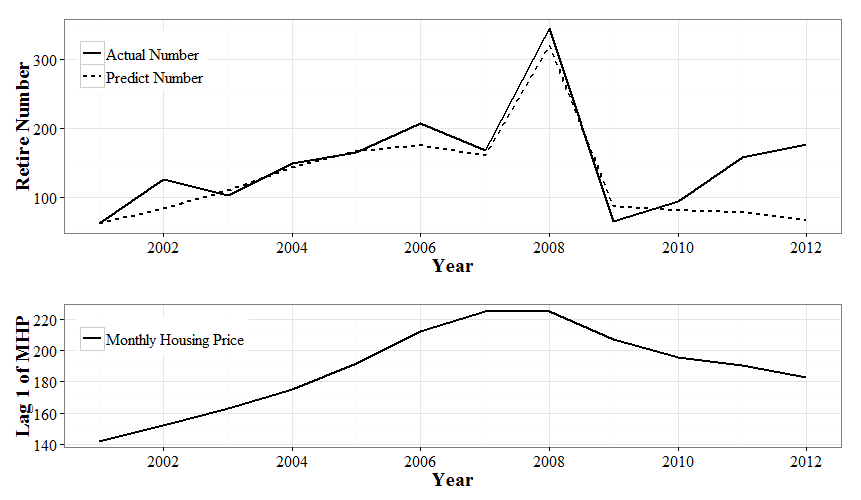
\includegraphics[width=0.5\textwidth]{MHP.png}}
   	\subfloat[Real Earnings]{\label{fig:Real}\includegraphics[width=0.5\textwidth]{realearnings.png}}
   	%\subfloat[Hazard function]{\label{fig:Hazard}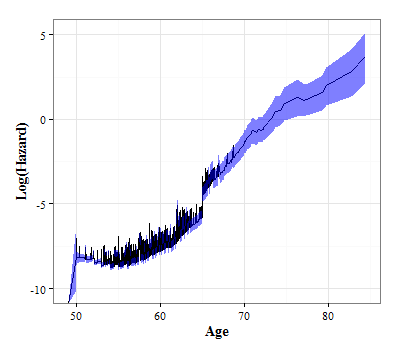
\includegraphics[width=0.35\textwidth]{loghazard.png}}
   	\caption{Economic Indicators and Retirement Predicting Plot}
   	\label{fig:EIndex}
   \end{figure}

   % Table generated by Excel2LaTeX from sheet 'Sheet4'
   \begin{table}[h!]
   	\centering
   	\scriptsize
   	\smallskip
   	\caption{Retirement Predictions by Occupational Code (OC) with External Variable.}
   	\begin{threeparttable}
   		\begin{tabular}{cL{1.2cm}L{1.2cm}L{1.2cm}L{1.2cm}L{1.2cm}L{1.2cm}L{1.2cm}L{1.2cm}L{1.2cm}l}
   			\toprule
   			Year  &  Crafts & Engineers& General Admin. & Laborers& Managers& Prof. Admin.& Operators& Scientists& Technicians& Total \\
   			\midrule
   			2001  & 23 (16) & 13 (10) & 4 (1) & 7 (5) & 15 (14) & 11 (9) & 8 (2) & 2 (1) & 5 (4) & 88 (62) \\
   			2002  & 23 (29) & 12 (16) & 4 (15) & 6 (11) & 15 (26) & 10 (18) & 8 (6) & 2 (1) & 5 (4) & 85 (126) \\
   			2003  & 23 (26) & 13 (13) & 5 (5) & 6 (6) & 13 (21) & 12 (13) & 10 (15) & 3 (2) & 6 (2) & 91 (103) \\
   			2004  & 32 (32) & 18 (23) & 7 (9) & 9 (7) & 16 (30) & 18 (25) & 11 (15) & 3 (3) & 8 (6) & 122 (150) \\
   			2005  & 40 (39) & 24 (17) & 8 (13) & 10 (7) & 21 (27) & 26 (31) & 12 (15) & 4 (4) & 11 (12) & 156 (165) \\
   			2006  & 35 (58) & 25 (29) & 6 (10) & 9 (9) & 21 (32) & 29 (37) & 10 (13) & 3 (4) & 9 (15) & 147 (207) \\
   			2007  & 24 (44) & 19 (25) & 9 (9) & 8 (9) & 24 (26) & 35 (40) & 10 (6) & 3 (4) & 9 (6) & 140 (169) \\
   			2008  & 50 (71) & 29 (33) & 19 (20) & 20 (12) & 57 (63) & 72 (84) & 27 (32) & 5 (7) & 19 (23) & 298 (345) \\
   			2009  & 13 (14) & 8 (6) & 6 (3) & 6 (7) & 17 (8) & 22 (10) & 7 (11) & 1 (1) & 5 (5) & 85 (65) \\
   			2010  & 10 (19) & 8 (17) & 5 (1) & 4 (8) & 16 (23) & 19 (16) & 5 (4) & 1 (3) & 4 (3) & 72 (94) \\
   			2011  & 25 (36) & 16 (25) & 14 (8) & 10 (9) & 40 (27) & 47 (34) & 11 (5) & 2 (1) & 10 (13) & 175 (158) \\
   			2012  & 29 (29) & 21 (23) & 16 (11) & 12 (10) & 51 (46) & 64 (36) & 14 (4) & 3 (2) & 13 (16) & 223 (177) \\
   			\bottomrule
   		\end{tabular}%
   		\begin{tablenotes}
   			\item[1] the number before the parentheses is predicted retirement number.
   			\item[2] the number inside the parentheses is actual retirement number.
   		\end{tablenotes}
   	\end{threeparttable}
   	\label{tab:EIcocs}%
   \end{table}%


   Unadjusted Monthly Housing Price (MHP) is another influential index and inclusion in the model resulted in the lowest MAPE value. Fluctuations in the lag also correlate strongly with the retirement number as shown in Figure \ref{fig:MHP}. However, the retirement number does not decrease coinciding with the decreasing of MHP after the 2008 financial crisis.



%%%%%%%%%%%%%%%%%%%%%%%%%%%%%%%%%%%%%%%%%%%%%%%%%%%%%%%%%%%%%%%%
\subsection{Models for Voluntary Quitting without External Economic Variables}

%I. dependent variable are YCSH, because age is not able to predict well. Why plot YCSH by vq and age by vq to describe why.
%one employee quit with 67 years old and less than 85 points. all quit before 65 years.
%II. shorten the length of risk set. how to shorten the risk set.
%iii. model comparison. (survival model, time series model, and logistic regression model)

A second area of interest in analyzing turnover is voluntary quitting.  Using the same methodology and set of variables applied to retirement modelling, we constructed a predictive model for quitting. The challenge of modelling quitting in the current context is that the current data has approximately 600 out of 8000 employees quitting during the 10-year study window resulting in a very high proportion of censored data.  With this data density, the model cannot generate a smooth baseline to achieve a good forecasting model using age as the dependent variable because employees quit across such wide range of ages (20 to 64); see Figure \ref{fig:agevq} and Table \ref{tab:vqmodelstats}.  Modelling years of service (YCS) as the dependent variable compresses the reference frame leading to better estimates with employees usually quitting within the first 10 years of service as shown in Figure \ref{fig:ycsvq}. Since an employee will not quit if they are eligible for pension, we remove those employees from the risk set when they meet either one of the requirements for retirement.  With those cases now censored, the indicators P85 and A65 are no longer useful for modelling.
\begin{figure}[h!]
	\centering
	\subfloat[Age at Quitting]{\label{fig:agevq}\includegraphics[width=0.5\textwidth]{vq_age_hist.png}}
	\subfloat[YCS at Quitting]{\label{fig:ycsvq}\includegraphics[width=0.5\textwidth]{vq_ycs_hist.png}}
	%\subfloat[Hazard function]{\label{fig:Hazard}\includegraphics[width=0.35\textwidth]{loghazard.png}}
	\caption{Histogram of Age and YCS at Quitting}
	\label{fig:vqhist}
\end{figure}
Among all the models shown in Table \ref{tab:vqmodelstats}, model [FILL IN NUMBER] with DIV, OC, AGEC, and ERIP as explanatory variables fits best.  A discrete version of the Cox model based on logistic regression also performs well with both models showing similar MAPE and $G_2$ values; see \citet{allison2010} for more detail on discrete models.

\begin{table}[htbp]
	\scriptsize
	\caption{Voluntary Quitting Models Statistics}
	\renewcommand{\arraystretch}{1.5}
	\renewcommand{\arraystretch}{1.5}
	\begin{tabular}{L{0.5cm}L{2cm}L{2.5cm}llllllll}
		\toprule
		\multicolumn{1}{c}{\textbf{No.}} &\multicolumn{1}{L{2cm}}{	\textbf{Dependent Variables}} &\multicolumn{1}{L{2.5cm}}{	\textbf{Independent Variables}}  &\multicolumn{1}{c}{\textbf{LR}}   &\multicolumn{1}{c}{\textbf{AIC}}  & \multicolumn{1}{c}{\textbf{SBC}}   & \multicolumn{1}{c}{\textbf{\begin{tabular}[c]{@{}c@{}}Pred. \\ MAPE\end{tabular}}} & \multicolumn{1}{c}{\textbf{\begin{tabular}[c]{@{}c@{}}Holdout \\ MAPE\end{tabular}}} &\multicolumn{1}{c}{\textbf{\begin{tabular}[c]{@{}c@{}}Pred. \\ $G^2$\end{tabular}}} & \multicolumn{1}{c}{\textbf{\begin{tabular}[c]{@{}c@{}}Holdout \\ $G^2$\end{tabular}}}  \\
		\midrule
	1    &	AGE &	DIV GENDER OC YCSH ERIP &  1226.8  & 5960.1 & 6041.4 & 83.7 & 91.35 & 1213.96 & 197.21 \\
	2    &	YCS & DIV OC AGEC ERIP&  1012.4 & 6848.5  & 6929.7 & 23.90 & 21.05 & 65.63 & 2.48 \\
		%YCS (Dependent) reduced the riskset &     & 1012.4 & 6848.5& 6929.7 & 21.11 & 21.12 & 32.85 & 3.32 \\
	3    & YCS reduced riskset & DIV OC AGEC ERIP &  838.4 1 & 6911.2 & 6992.5 & 15.16 & 18.77 & 26.25 & 2.08 \\
	4    & Logistic regression  &DIV OC AGEC ERIP&  1870.7& 4712.6  & 4938.6 & 15.98 & 17.55 & 23.03 & 3.21 \\
	5    &	Time series  &  & NA    & NA    & NA  &    26.41 & 61.32 & 30.88 & 18.33 \\
		\bottomrule
	\end{tabular}%
	\label{tab:vqmodelstats}%
\end{table}%

Our results suggest that voluntary quitting is influenced by an employee's age at the start of their service. The coefficient estimate for age is -0.025. As the reference age is 35.44, this means that the hazard of quitting for an employee that started working at age 36.44 is $exp(-.025)=.975$ that of an employee starting at age 35.44. For each additional year of age at beginning of service we estimate 2.5\% drop in hazard of quitting. The employee's survival probability at any time, $t$, can be computed as $S(t)^{1.025} = (S(t)^{e^{0.025}})$ if age is one year below average, where $S(t)$ is the baseline survival probability for a reference employee of average age at initial employment. Moving in the other direction, the employee's survival probability increases to $S(t)^{0.975}=(S(t)^{e^{-0.025}})$ for a one year increase in the employee's starting age. Together, this implies that at any given voluntary quitting age, the employee who starts earlier is more likely to quit than an equivalent employee who starts working later.

The early retirement incentive option ERIP also shows a significant impact on an employee's quitting behavior.  The coefficient for this indicator was 1.111 leading to a hazard ratio of $e^{.1.111} = 3.04$.  This indicates that, on average, an individual's hazard of quitting increased by almost 3 times during this period.  It is unclear why an optional early retirement program would influence quitting but it is possible that the program led to leadership or organizational disruptions [NEED CITATION HERE] or simply that it took place during  2008, a time of significant economic upheaval due to rapidly changing external economic conditions.

The DIV variable was also a significant predictor.  For analysis, the baseline level was chosen arbitrarily as division 6 so that it's hazard rate is determined by the baseline.  Relative to this baseline, division 7 has a similar hazard of quitting according to the model estimates. Conversely, the other divisions all have negative coefficients with hazard ratios less than 1 indicating that individuals within these groups have lower hazard of quitting than group 6.

The OC variable was another significant predictor. For analysis, the baseline level was engineer for this variable so that it's hazard rate is determined by the baseline. Relative to this group, all the other divisions have negative coefficients with hazard ratios less than 1. In particular, the crafts group with coefficient of -1.165 and a hazard ratio of 0.312 shows a much lower hazard of quitting than the engineering group.  This may reflect that differences in sociological or demographic factors among workers in these job categories, differences in compensation relative to other opportunities, or other differences in local or national economic mobility.

In general, differences in quitting rates could be caused by differences in age demographics, leadership, departmental and job function, or departmental leadership.

The baseline survival function and log hazard function for quitting are shown in Figure \ref{fig:vqbasepred}. The survival probability decreases steeply between 0 and 10 years of service. By 10 years of service at 10 the survival probability has decreased to close to 0.25, which indicates that 75\% of employees quit within the first 10 years of service.  The slope of survival function flattens to 0 from 10 to 30 years of service.  Accompanying the survival function is the log of the cumulative hazard ratio.  Again, the steep rise in the cumulative hazard between years of service at 0 to 10 indicates the increased quitting activity during this period.  Afterward the cumulative hazard levels off indicating a drop in the hazard rate at these future points.



\begin{table}[htbp]
	\centering
	\scriptsize
	\renewcommand{\arraystretch}{1.5}
	\caption{Parameter Estimates for Voluntary Quitting Models}
	\begin{threeparttable}
		\begin{tabular}{llL{2.5cm}L{1.5cm}L{2.5cm}L{1.5cm}}
			\toprule
			&       & \multicolumn{2}{c}{\textbf{Model w/o external variable}} & \multicolumn{2}{c}{\textbf{Model with Real Dividend}} \\
			\hline
			Parameter &   Label & Parameter (Standard Error) & Hazard Ratio & Parameter (Standard Error) & Hazard Ratio \\
			\midrule
			DIV & Div1  & -3.066 (0.263)*** & 0.047 & -3.305 (0.269)*** & 0.037 \\
			DIV & Div2  & -2.652 (0.198)*** & 0.071 & -2.875 (0.204)*** & 0.056 \\
			DIV & Div3  & -3.015 (0.253)*** & 0.049 & -3.258 (0.258)*** & 0.038 \\
			DIV & Div4  & -2.533 (0.288)*** & 0.079 & -2.769 (0.292)*** & 0.063 \\
			DIV & Div5  & -2.739 (0.314)*** & 0.065 & -2.934 (0.317)*** & 0.053 \\
			DIV & Div7  & 0.028 (0.145) & 1.029 & 0.101 (0.146) & 1.107 \\
			DIV & Div8  & -0.806 (0.157)*** & 0.447 & -0.968 (0.163)*** & 0.38 \\
			DIV & Div9  & -3.985 (0.586)*** & 0.019 & -4.207 (0.588)*** & 0.015 \\
			DIV & Div10 & -1.325 (0.136)*** & 0.266 & -1.5 (0.142)*** & 0.223 \\
			OC  & C     & -1.163 (0.274)*** & 0.313 & -1.11 (0.275)*** & 0.329 \\
			OC  & G     & -0.794 (0.198)*** & 0.452 & -0.796 (0.198)*** & 0.451 \\
			OC  & L     & -0.711 (0.228)** & 0.491 & -0.619 (0.229)** & 0.539 \\
			OC  & M     & -0.541 (0.15)*** & 0.582 & -0.497 (0.15)*** & 0.609 \\
			OC  & P     & -0.53 (0.135)*** & 0.588 & -0.506 (0.136)*** & 0.603 \\
			OC  & R     & -0.95 (0.308)** & 0.387 & -0.886 (0.309)** & 0.412 \\
			OC  & S     & -0.691 (0.275)* & 0.501 & -0.682 (0.276)* & 0.506 \\
			OC  & T     & -0.608 (0.203)** & 0.544 & -0.564 (0.204)** & 0.569 \\
			AGEC &       & -0.025 (0.005)*** & 0.975 & -0.026 (0.005)*** & 0.974 \\
			ERIP  & 1     & 0.851 (0.135)*** & 2.343 & 0.479 (0.149)** & 1.614 \\
			Real Dividends &       &       &       & 0.085 (0.017)*** & 1.089 \\
			\bottomrule
		\end{tabular}%
		\begin{tablenotes}
			\item[1] * denotes $P<0.05$, ** denotes $P<0.01$, and *** denotes $P<0.001$.
		\end{tablenotes}
		
	\end{threeparttable}
	\label{tab:vqparaest}%
\end{table}

\begin{figure}[h!]
	\centering
	\subfloat[Survival Function]{\label{fig:vqsurv}\includegraphics[width=0.5\textwidth]{VQSURV.png}}
	\subfloat[Log of Cumulative Hazard]{\label{fig:vqcumh}\includegraphics[width=0.5\textwidth]{VQlogcumhaz.png}}
	%\subfloat[Cumulative Hazard]{\label{fig:vqcum}\includegraphics[width=0.35\textwidth]{VQCUM.png}}
	\caption{Voluntary Quitting Model Baselines with 95\% Confident Intervals}
	\label{fig:vqbasepred}
\end{figure}


%\begin{figure}[h!]
%	\centering
%	\includegraphics[width=0.6\textwidth]{vq.png}
%	\caption{Voluntary Quitting Forecasting}
%	\label{fig:predictvq}	
%	
%\end{figure}

\begin{table}[h!]
	\centering
	\scriptsize
	\smallskip
	\caption{Voluntary Quitting Predictions by Occupational Code (OC) without external variables}
	\begin{threeparttable}
		\begin{tabular}{cL{1.2cm}L{1.2cm}L{1.2cm}L{1.2cm}L{1.2cm}L{1.2cm}L{1.2cm}L{1.2cm}L{1.2cm}l}
			\toprule
			Year  &  Crafts & Engineers& General Admin. & Laborers& Managers& Prof. Admin.& Operators& Scientists& Technicians& Total \\
			\midrule
			2001  & 3 (2) & 12 (14) & 4 (2) & 4 (3) & 8 (12) & 11 (16) & 2 (0) & 2 (2) & 4 (1) & 49 (52) \\
			2002  & 2 (1) & 13 (10) & 3 (3) & 3 (2) & 7 (8) & 11 (11) & 1 (0) & 1 (4) & 3 (5) & 45 (44) \\
			2003  & 2 (0) & 17 (13) & 3 (1) & 4 (2) & 7 (14) & 12 (10) & 1 (1) & 1 (5) & 3 (2) & 51 (48) \\
			2004  & 2 (2) & 23 (20) & 4 (4) & 3 (2) & 7 (5) & 12 (12) & 1 (0) & 1 (1) & 4 (3) & 57 (49) \\
			2005  & 1 (5) & 23 (23) & 3 (3) & 2 (2) & 7 (8) & 11 (18) & 1 (0) & 1 (0) & 3 (4) & 53 (63) \\
			2006  & 1 (1) & 22 (32) & 2 (2) & 1 (2) & 6 (6) & 10 (16) & 1 (3) & 1 (1) & 2 (2) & 46 (65) \\
			2007  & 1 (2) & 17 (29) & 2 (3) & 1 (2) & 6 (6) & 9 (14) & 1 (2) & 1 (0) & 2 (2) & 39 (60) \\
			2008  & 1 (2) & 23 (34) & 5 (5) & 2 (0) & 11 (4) & 19 (18) & 2 (5) & 3 (1) & 4 (5) & 69 (74) \\
			2009  & 1 (1) & 9 (16) & 2 (4) & 1 (5) & 5 (4) & 9 (6) & 1 (0) & 1 (1) & 2 (3) & 29 (40) \\
			2010  & 1 (1) & 9 (13) & 3 (7) & 1 (4) & 4 (4) & 9 (2) & 1 (2) & 1 (1) & 2 (4) & 30 (38) \\
			2011  & 1 (0) & 8 (9) & 3 (4) & 1 (2) & 3 (3) & 9 (3) & 1 (0) & 1 (2) & 1 (1) & 29 (24) \\
			2012  & 1 (1) & 8 (6) & 3 (7) & 1 (0) & 3 (4) & 10 (14) & 1 (0) & 1 (2) & 2 (2) & 30 (36) \\
			\bottomrule
		\end{tabular}%
		\begin{tablenotes}
			\item[1] the number before the parentheses is predicted retirement number.
			\item[2] the number inside the parentheses is actual retirement number.
		\end{tablenotes}
		
	\end{threeparttable}
	\label{tab:VQcocscode}
\end{table}

\subsection{A Model for Voluntary Quitting including external economic variables}
i. tested which variable does significantly impact on employee voluntary quit.
Because voluntary quitting is more sensitive affected by macro economics, we further examined the external variables using the counting process model with yearly interval based on calendar year to test their effects on voluntary quitting. This model has the similar parameter estimation as the selected model as shown in the right part of the Table \ref{tab:vqparaest}. We found one indicators are statistically significant and also improve the model forecasting due to lower MAPE and $G^2$ than the values of selected model without economic indicator, which is Real Dividend as shown in Table \ref{tab:vqEI}. According to the estimates of Table \ref{tab:EI}, Real dividend is the most important factor among all the indicators as it has lowest $G^2$ and MAPE. The test results show that it has strong impact on the quitting behaviors. As shown in Figure \ref{fig:vqrealdividend}, the fluctuation of voluntary quitting plot is corresponding with 1 year lag of the trend of Real dividend.



%Another alternative eligibility criteria occurs when individuals exceed an age of 65 years and so we would anticipate the hazard increasing at this point in an employees career.  Because the response variable in our model is age, we cannot estimate the effect of this within the proportional hazards setting because the impact is included in the baseline hazard which should increase after this point; see Figure \ref{fig:basepred} (explain).  However, by including an interaction between the Age 65 and points 85 indicator, we can estimate how the impact of reaching 85 points diminishes beyond regular retirement age.  In this case, the interaction term is estimated at -1.61 leading to a decreasing effect of the 85 points criteria to $e^{1.44-1.61} = 0.84$ indicating that people that exceed both criteria actually have a reduced hazard of retiring over those have only met the Age 65 criteria.  In other words, the fact that the individual remains on the job after hitting either criteria indicates that the other criteria has less impact (or that they are intending to work longer).



%According to our model, retirement can also be influenced by employee's age and their years of service at the time of hiring (YCSH).  The estimates for age are -0.17. As the reference age is 45.49, it means the employee's survival probability is $S(t)^{1.19}(S(t)^{e^{0.17}})$ when the employee started age is one year younger than 45.49,  where $S(t)$ is the baseline survival probability at time t for a reference employee of average age, in the case 45.49 years old at the start of the current interval. The employee's survival probability is $S(t)^{0.84}(S(t)^{e^{-0.17}})$ for every one year increase beyond 45.49 in the employee's starting age. This indicates that at any given age, the employee who starts earlier than 45.49 years old is more likely to retire , because they have more years of service and are much likely to reach retirement requirement (85 points) earlier than the employee who starts at older age. Similar as the years of service, the employee's years of service are hiring time has positive estimates (0.019) with the hazard ratio (1.019). It leads to $S(t)^{0.98}$ of the survival probability for every one year decreasing of the employee in the reference years of service at time of hiring. On the other hand, the survival probability is $S(t)^{1.019}$ for every one year increase of the employee in the reference years of service at hiring time. This indicates that the employee who has more years of service are more likely to retire than the employee who has less years of service.

%In the fiscal year 2008, the employer in the study created a temporary early retirement buyout option. The response window for this option was 3 months although the specific details of this are unknown. In order to deal with the increased level of retirement during this period we including a time dependent indicator variable.  The coefficient for this indicator was 0.86 leading to a hazard ratio of 2.21 which indicates that, on average, an individuals hazard of retirement increased by almost 2.2 times during this period.  If more information were known about the requirements or targets of this policy, a more case specific estimate would be possible.  However, this would not effect the overall aggregate retirement estimates.  It is important to include this one-time effect in order to improve the estimates of other factors(work on this last part - why do we need to include). We further test the policy effect on the employee who are eligible for getting pension. The test results shows the policy had a significant effect for the employee who are eligible for getting the full pension benefit rather than the employee who are eligible for getting partial retirement plan as the interaction term of between policy and points 75 or points 65 are not statistically significant. The hazard ratio for the policy effect on those employee substantially increase to 15.85 from 2.21, which is more than seven times of the basic policy effect, after the model adding a interaction term of policy and points 85.

%Another significant factor is division as shown in the table \ref{tab:paraest.}. As the results shows the employees in some division has positive parameter estimates which is division 6, 7 and 8. Two divisions (division 6 and 7) have very high hazard ratio: 8.46 and 11.42, which indicates that the employee in division 6 and division 7 are much more likely to retire than the employee in reference division (1). Three divisions (2, 3, and 9) have negative estimates (-0.97, -0.24, and -3.02) and the hazard ratios lower than 1 (0.38, 0.79, and 0.05), which indicates the employee in those divisions are much less likely to retire than the employee in reference division (1). Two divisions (4 and 5) are not statistically significant, which indicates that the employee in division 4 and 5 has the similar chance to retire with the employee in the reference division (1). The diversity retirement behavior among divisions might be caused by the diversity of the demographic structure, leadership, departmental function, and departmental culture,

%The baseline survival function and log hazard function are shown in Figure \ref{fig:basepred}. The survival probability is 1 before age 49 as shown in Figure \ref{fig:Surv}, which indicates that no employee retire before age at 49. Survival probability starts to slowly decease from age 50 to age 62. The survival probability is around 0.75 for the employee who less than 62 years old, which indicates the employee who is less than 62 years has a probability of 25\% to retire.  The slope of survival function decrease sharply and causes the survival probability steeply decreasing from 0.75 to almost 0 from age 62 to age 70, which indicates the employee are much more likely to retire from age 62 to 70. Accompany with the survival function, the log hazard ratio starts to rise up from age 62 and it steps up at age 65 as shown in Figure \ref{fig:Hazard}. The trend for hazard function tend to increase by age increasing. The hazard ratio causes the employee retire probability increasing sharply.




%\item Employee Profile 1: The employee's pattern for employees retire right away.

%\item Employee Profile 2: The employee's pattern who did not retire after eligible for retirement.

%\item New Chapter: Short term prediction model.  Logistic regression for 1 year on elgible retirees.  Possible prediction?



\begin{table}[]
	\scriptsize
	\centering
	\caption{Economic Index Test Statistics for Voluntary Quitting}
	\begin{threeparttable}
		\begin{tabular}{@{}llllll@{}}
			\toprule
			\textbf{Economic Inidcator}\tnote{1} &\multicolumn{1}{c}{\textbf{$\chi^2$}} &  \multicolumn{1}{c}{\textbf{P-value}} & \multicolumn{1}{c}{\textbf{\begin{tabular}[c]{@{}c@{}}Hazard \\ ratio\end{tabular}}}   &  \multicolumn{1}{c}{\textbf{MAPE}} &\multicolumn{1}{c}{\textbf{$G^2$}} \\ \midrule
			Without Econmic indicator &            &                &              & 15.71 & 28.33 \\
			MHP                   & 37.93      & \textless.001  & 1.012        & 13.62 & 18.44 \\
			SAMHP                    & 37.75      & \textless.001  & 1.012        & 13.64 & 18.50 \\
			SEMHP         & 39.80      & \textless.001  & 1.020        & 13.74 & 18.67 \\
			SESAMHP          & 39.63      & \textless.001  & 1.020        & 13.75 & 18.68 \\
			S\&P500                     & 0.02       & 0.879          & 1.000        & 15.46 & 27.79 \\
			Dividend                  & 31.21      & \textless.001  & 1.077        & 13.01 & 18.01 \\
			Earnings                  & 8.83       & 0.003          & 1.009        & 15.81 & 23.88 \\
			Consumer Price Index      & 35.84      & \textless.001  & 1.024        & 24.26 & 42.95 \\
			Real Price                & 5.34       & 0.021          & 1.000        & 17.94 & 34.52 \\
			Real Dividend             & 26.66      & \textless.001  & 1.089        & 12.40 & 16.37 \\
			Real Earnings             & 3.71       & 0.054          & 1.005        & 14.16 & 23.34 \\
			Long Interest Rate        & 12.04      & 0.001          & 0.789        & 19.10 & 38.73 \\
			Unemployment Rate         & 2.99       & 0.084          & 1.068        & 17.04 & 34.96 \\
			P/E 10                     & 16.22      & \textless.001  & 0.968        & 17.95 & 35.19 \\
			Wilshire5000              & 10.75      & 0.001          & 1.031        & 15.84 & 21.31 \\ \bottomrule
		\end{tabular}
		\begin{tablenotes}
			\item[1] it is the selected model without economic indicator.
		\end{tablenotes}
	\end{threeparttable}
	\label{tab:vqEI}%
\end{table}

\begin{figure}
	\centering
	\includegraphics[width=0.5\textwidth]{realdividend.png}
	\caption{Voluntary Quitting with Real Dividend}
	\label{fig:vqrealdividend}
\end{figure}

\begin{table}[h!]
	\centering
	\scriptsize
	\smallskip
	\caption{Voluntary Quitting Predictions by Occupational Code (OC) with External Variables}
	\begin{threeparttable}
		\begin{tabular}{cL{1.2cm}L{1.2cm}L{1.2cm}L{1.2cm}L{1.2cm}L{1.2cm}L{1.2cm}L{1.2cm}L{1.2cm}l}
			\toprule
			Year  &  Crafts & Engineers& General Admin. & Laborers& Managers& Prof. Admin.& Operators& Scientists& Technicians& Total \\
			\midrule
		     2001  & 3 (2) & 12 (14) & 3 (2) & 4 (3) & 7 (12) & 10 (16) & 2 (0) & 1 (2) & 4 (1) & 46 (52) \\
		     2002  & 2 (1) & 11 (10) & 2 (3) & 3 (2) & 6 (8) & 8 (11) & 1 (0) & 1 (4) & 3 (5) & 37 (44) \\
		     2003  & 2 (0) & 14 (13) & 2 (1) & 3 (2) & 6 (14) & 9 (10) & 1 (1) & 1 (5) & 3 (2) & 41 (48) \\
		     2004  & 1 (2) & 20 (20) & 3 (4) & 3 (2) & 6 (5) & 10 (12) & 1 (0) & 1 (1) & 3 (3) & 47 (49) \\
		     2005  & 1 (5) & 22 (23) & 3 (3) & 2 (2) & 6 (8) & 10 (18) & 1 (0) & 1 (0) & 3 (4) & 50 (63) \\
		     2006  & 1 (1) & 24 (32) & 2 (2) & 1 (2) & 7 (6) & 10 (16) & 1 (3) & 1 (1) & 2 (2) & 50 (65) \\
		     2007  & 1 (2) & 21 (29) & 2 (3) & 1 (2) & 7 (6) & 11 (14) & 1 (2) & 2 (0) & 2 (2) & 48 (60) \\
		     2008  & 1 (2) & 22 (34) & 5 (5) & 2 (0) & 11 (4) & 20 (18) & 2 (5) & 3 (1) & 4 (5) & 69 (74) \\
		     2009  & 1 (1) & 13 (16) & 4 (4) & 1 (5) & 7 (4) & 15 (6) & 1 (0) & 2 (1) & 2 (3) & 47 (40) \\
		     2010  & 1 (1) & 10 (13) & 3 (7) & 1 (4) & 5 (4) & 11 (2) & 1 (2) & 1 (1) & 2 (4) & 35 (38) \\
		     2011  & 1 (0) & 7 (9) & 2 (4) & 1 (2) & 3 (3) & 8 (3) & 1 (0) & 1 (2) & 1 (1) & 25 (24) \\
		     2012  & 1 (1) & 8 (6) & 3 (7) & 1 (0) & 3 (4) & 11 (14) & 1 (0) & 1 (2) & 2 (2) & 30 (36) \\
		
			\bottomrule
		\end{tabular}%
		\begin{tablenotes}
			\item[1] the number before the parentheses is predicted retirement number.
			\item[2] the number inside the parentheses is actual retirement number.
		\end{tablenotes}
		
	\end{threeparttable}
	\label{tab:VQEIcocscode}
\end{table}


\section{Conclusions and Managerial Implications}

Generally, we found that using the Cox proportional hazards model along with appropriately chosen internal and external variables led to accurate predictions of retirement.  In the training sample we found that prediction error as measured by MAPE was approximately 25\% while the predictions in the smaller 2 year holdout window were approximately 5\%.  Although this included only two validation points, these results indicate that the method has good potential [LETS USE A GAINS CHART OR PRECISION RECALL OR SOMETHING].  The key internal variables that improved model predictions include division, years of service at hire (YCSH), and age at hire (AGEH).  In addition, S\&P 500 real earnings also showed a significant association with risk of retirement although the magnitude at approximately 1.3\% was (greater or less) than other effects for small changes.  We also find that retirement hazard increases significantly when an individual hits 85 points of retirement credit and is eligible for full benefits but then reverts back to a lower hazard after age 65.  Furthermore, the the early retirement incentive plan implemented by the organization in 2008 had a major impact with a large increase in the hazard of retirement, particularly for those that were eligible for full benefits with points exceeding 85.  In terms of prediction, in out-of-sample tests, taking into account individual and external information provides a significant improvement over more traditional forecasting methods.  It also provides useful predictions on subgroups that are not possible for standard forecasting models.

Quitting behavior differed significantly by division, occupation, and age at start of service, which reflects both differences in worker satisfaction across the organization, and by job type. Age connects logically since, for a given number of years of service, the employee that starts earlier, will be younger and, therefore, may see a more significant long term opportunity in a new position elsewhere.  The 2008 early retirement incentive program was also correlated with a significant amount of quitting.  It is unclear if the higher hazard of quitting was directly due to disruptions, management or otherwise, caused by the accelerated retirements or was related somehow to the drastic economic changes during that time period.  In terms of predictive power, the quitting model performs well with MAPE in the training sample estimated at 15.16\% and 18.77\% in the holdout sample[GAINS CHART HERE ALSO].  Both estimates are far superior to traditional forecasting techniques.  As with retirement, external information in the form of S\&P real corporate dividends were positively correlated with quitting indicating that as profits at large private sector companies increase, the hazard of quitting rises significantly.


Drawing on this list of findings, this work provides a number of valuable managerial implications.  Foremost, this work shows that fairly accurate survival model based retirement prediction is feasible in large organizations when defined benefit plans are in place.  These models are accurate enough to provide useful predictive visibility for human resources management professionals.  Such models are of particular value when a large portion of the workforce has specialized skills that require an extensive search process to replace or if the organization requires long lead times in the hiring process due to security or other concerns.  The model also provides guidance as to expected retirement and quitting behavior across subgroups of the organization. Significant deviations from these expectations, particularly  in terms of  abnormal quitting behavior, may indicate the need for management intervention.  Finally, such models can alert managers to key external factors that may indicate increases in retirement or quitting behavior.  The use of lagged variables may allow management to craft incentive policies in response to changes in the external economy.

Although this study brings to light much, it is important to consider a number of limitations due to the data and models used.  The data were sampled based on a specific time window leading to a truncated sample which limits the modeling approaches.  In addition,  it would be beneficial to have have a longer prediction window to validate the model.  Variables such as salary, and more carefully documented division data, which would be available within the sponsoring organization, could strengthen the results presented here.  In the same vein, more complete internal organizational details on early retirement incentive program as well as details of the defined benefit plan could improve the quality of inferences in this study.  Finally, the accuracy of results for the retirement portion of this study are based on the specific nature of the defined benefit pension dominant during the period of study.  The accuracy of predictions observed in this study may not generalize to organizations offering defined contribution retirement plans although a similar methodology may still prove useful in generating predictions.


In terms of the model, although tested, the proportional hazards assumption may be violated for some effects.  In addition, variability in the baseline estimator can cause overestimation of hazard and more sophisticated smoothed baseline models may be beneficial in this case.

This work contributes significantly to both practical and academic literature on factors affecting retirement and management of staffing through predictive models. We expect that future work will continue to develop and improve the modeling techniques and result in better explanatory models for academic research as well as functioning systems for industry.  Furthermore, we believe that the current methods can be extended to include qualitative and survey based longitudinal feedback from employees through the time varying covariate methodology.  The addition of such attitudinal data may provide significant additional value to both academic and industry practitioners.


	\bibliographystyle{abbrvnat}%Choose a bibliograhpic style%
	\bibliography{Bib}
\end{document}


1) Restate and Summarize key findings above.
2) Interpret the findings.
3) So What?  Importance of the findings. Managerial implications. What can the model do?
  How should they use it?  Good, bad, etc.
3) Possible limitations of study
4) Next steps/future work.
5)

Several key questions:
\begin{enumerate}
	\item How accurately can retirement(quitting) be predicted?  Summarize the results of the predictions overall.
    \item How many employees will retire(quit) next year by occupational category and/or division?  Summarize the table.
	\item What factors indicate an individual is more likely to retire(quit)?
retire = division, year of service at hire, age at hire, ERIP, points = 85 and age=65 interaction term.
quitting = division, occupation, age at start of years of service, ERIP.
	\item Which external economic factors are most predictive of retirement or quitting?
 retirement = real earnings, quitting = real dividends
	\item What is the magnitude  of impact of an Early Retirement Incentive Programs (ERIP)?  Significant impact on both retirement and quitting in that year.  Why?  Explain dynamics including interaction ERIP*points term for retirement.  Why should it affect quitting.
	\item How do the tenure and age impact retirement?  Tell the story, early tenure folks are more likely to quit.  Quitting is associated with high real dividends which indicates a robust job market with companies highly profitable.  As individuals age risk (hazard) of quitting decreases as they become closer to retirement/pension eligibility age. Late in their careers, as the achieve full retirement benefit points, they become more likely to retire and are highly impacted by ERIP programs.  Nevertheless, for those that choose to stay beyond age 65, the hazard of retirement recedes to more normal levels.  Most choose to retire by age 70.

\item Details about model fitting.

\end{enumerate}


1) Specialized organization.  Behavior of these employees may not generalize.
2) Retirement data based on defined benefit plans.  Behavior may differ significantly for defined contribution.
3) Left truncation would be alleviated if the population data was provided.  In such a case alternative models could have been implemented.
4) Limitations of PH model: Baseline is not smooth.
5)Additional data would benefit: more detailed knowledge of ERIP convenants, salary information, changes in department structure.


2) Practical findings were provided above and should be valuable to organizations managing human resources.
3) Results provide evidence of specific external variables impacting retirement.
4) Major contribution is model development techniques which can be extended to develop richer and better explanatory models for academic research as well as better predictions for actual managers.
5) The current work can be extended to include qualitative and survey based longitudinal feedback from employees through the time varying covariate methodology.  Again, this provides significant value to both academic and industry practitioners.





1) We were construct an individual level retirement model for current and past workers that accurately predicted yearly retirement levels.

2) A semi-parametric cox proportional hazards model was used to model age at retirement.  The model investigated demographic, organizational, and macroeconomic factors that might impact the retirement decision.

3) Factors that had the strongest influence included years of service, whether or not an ERP was in effect, whether or not the individual exceeded the number of points required for full retirement benefits.  The most valuable external factor impacting retirement decisions is the Real Earnings as defined by the bureau of labor statistics.

4) Discuss impacts captured by baseline.

5) Factors that did not seem to significantly impact retirement decisions included gender, payroll classification, job classification code, and a large number of additional macroeconomic indicators.

6) The model was tested and was able to accurately predict number of retirements up to two years into the future.  It may be accurate beyond that as well but sufficient data was not available to test this.

7) Why might real earnings be important.

8) Moderating effect of age.  Workers that stayed beyond the term required for full benefits were seen to have much reduced probabilities of retiring as indicated by a moderating interaction indicator.


Managerial Implications....
